\documentclass{book}
\usepackage{physics}
\usepackage{graphicx}
\usepackage{caption}
\usepackage{amsmath}
\usepackage{bm}
\usepackage{framed}
\usepackage{authblk}
\usepackage{empheq}
\usepackage{amsfonts}
\usepackage{esint}
\usepackage[makeroom]{cancel}
\usepackage{dsfont}
\usepackage{centernot}
\usepackage{mathtools}
\usepackage{bigints}
\usepackage{amsthm}
\theoremstyle{definition}
\newtheorem{defn}{Definition}[section]
\newtheorem{prop}{Proposition}[section]
\newtheorem{rmk}{Remark}[section]
\newtheorem{thm}{Theorem}[section]
\newtheorem{exmp}{Example}[section]
\newtheorem{prob}{Problem}[section]
\newtheorem{sln}{Solution}[section]
\newtheorem*{prob*}{Problem}
\newtheorem{exer}{Exercise}[section]
\newtheorem*{exer*}{Exercise}
\newtheorem*{sln*}{Solution}
\usepackage{empheq}
\usepackage{tensor}
\usepackage{xcolor}
%\definecolor{colby}{rgb}{0.0, 0.0, 0.5}
\definecolor{MIT}{RGB}{163, 31, 52}
\usepackage[pdftex]{hyperref}
%\hypersetup{colorlinks,urlcolor=colby}
\hypersetup{colorlinks,linkcolor={MIT},citecolor={MIT},urlcolor={MIT}}  



\newcommand*\widefbox[1]{\fbox{\hspace{2em}#1\hspace{2em}}}

\newcommand{\p}{\partial}
\newcommand{\R}{\mathbb{R}}
\newcommand{\C}{\mathbb{C}}
\newcommand{\lag}{\mathcal{L}}
\newcommand{\nn}{\nonumber}
\newcommand{\ham}{\mathcal{H}}
\newcommand{\M}{\mathcal{M}}
\newcommand{\I}{\mathcal{I}}
\newcommand{\K}{\mathcal{K}}
\newcommand{\F}{\mathcal{F}}
\newcommand{\w}{\omega}
\newcommand{\lam}{\lambda}
\newcommand{\al}{\alpha}
\newcommand{\be}{\beta}
\newcommand{\x}{\xi}

\newcommand{\G}{\mathcal{G}}

\newcommand{\f}[2]{\frac{#1}{#2}}

\newcommand{\ift}{\infty}

\newcommand{\lp}{\left(}
\newcommand{\rp}{\right)}

\newcommand{\lb}{\left[}
\newcommand{\rb}{\right]}

\newcommand{\lc}{\left\{}
\newcommand{\rc}{\right\}}


\newcommand{\V}{\mathbf{V}}
\newcommand{\U}{\mathcal{U}}
\newcommand{\Id}{\mathcal{I}}
\newcommand{\D}{\mathcal{D}}
\newcommand{\Z}{\mathcal{Z}}

%\setcounter{chapter}{-1}






\usepackage{subfig}
\usepackage{listings}
\captionsetup[lstlisting]{margin=0cm,format=hang,font=small,format=plain,labelfont={bf,up},textfont={it}}
\renewcommand*{\lstlistingname}{Code \textcolor{violet}{\textsl{Mathematica}}}
\definecolor{gris245}{RGB}{245,245,245}
\definecolor{olive}{RGB}{50,140,50}
\definecolor{brun}{RGB}{175,100,80}

%\hypersetup{colorlinks,urlcolor=colby}
\lstset{
	tabsize=4,
	frame=single,
	language=mathematica,
	basicstyle=\scriptsize\ttfamily,
	keywordstyle=\color{black},
	backgroundcolor=\color{gris245},
	commentstyle=\color{gray},
	showstringspaces=false,
	emph={
		r1,
		r2,
		epsilon,epsilon_,
		Newton,Newton_
	},emphstyle={\color{olive}},
	emph={[2]
		L,
		CouleurCourbe,
		PotentielEffectif,
		IdCourbe,
		Courbe
	},emphstyle={[2]\color{blue}},
	emph={[3]r,r_,n,n_},emphstyle={[3]\color{magenta}}
}


\begin{document}
\begin{titlepage}\centering
 \clearpage
 \title{{\textsc{\textbf{EXPERIMENTAL ATOMIC PHYSICS}}}\\ \smallskip - A Quick Guide - \\}
 \author{\bigskip Huan Q. Bui}
  \affil{B.A., COLBY COLLEGE (2021) $\,$\\  
  	MASSACHUSETTS INSTITUTE OF TECHNOLOGY}
 \date{June 15, 2021 - \today}
 \maketitle
 \thispagestyle{empty}
\end{titlepage}

\noindent \textbf{Preface}


$\,$\\


\noindent Greetings, \\


While I have spent most of my undergraduate years in Professor Charles Conover's lab at Colby College working on cold atom experiments, I never had \textit{formal} training in atomic, molecular, and optical physics. The closest to formal training I have for AMO physics is a standard quantum mechanics course I took in the fall of my junior year. Most of the intuition I have for atomic physics, I learned from my discussions with Professor Conover or read from books and articles here and there. This article is my attempt at \textit{formally} teaching myself this subject. It will mostly contain basic/essential concepts in AMO physics. I'll also sprinkle in a few ideas or definitions that are relevant to what I do in Prof. Zwierlein's group. \\

This article is my version of an ``atomic physics dictionary,'' which should keep growing as I go along in my education and research at MIT. As a result, there is no good way for me to organize the topics here but by alphabetical order (hence ``dictionary''). I don't know how well I'll be able to curate this article, but we'll see. As the title suggests, this article is about \textit{experimental} atomic physics. So I will try to include not just atomic physics theory but also experimental techniques/designs and some control and electronics theory. \\


In any case, enjoy and please feel free to report any errors!


\newpage




\chapter*{A}



\section*{Atomic coherence}

In physics, two systems are said to be coherent if their frequency and waveform are identical. Two waves are said to be coherent if they have a constant relative phase. Similarly, \textbf{atomic coherence} is the induced coherence between levels of a multi-level atomic system sometimes observed when it interacts with a coherent electromagnetic field.\\


Atomic coherence is often discussed in the context of Rabi flopping. If a coherent, narrow bandwidth laser is applied to a two-level system, Rabi floppings between the ground and excited state populations occur. Now consider a system comprised of a large collection of identical two-level systems. All such systems will begin Rabi oscillation at the same time under the application of the mentioned laser source, and all of them will be in phase with each other. The system is coherent. However, after some finite time $t$, different atoms return to their ground states (via spontaneous decay) at different times, and Rabi oscillations begin to go out of phase. As time passes by, fewer atoms will be in phase. This is decoherence. \\

The coherence time is the time over which the system maybe considered coherent. 

\section*{Avoided crossing} 


\begin{figure}[!htb]
	\centering
	\includegraphics*[width=0.75\textwidth]{images/avoided_crossing}
	\caption{From Wikipedia}
\end{figure}


This concept is actually mathematically very easy to describe. Basically, avoided crossing is a phenomenon where two eigenvalues of a Hermitian matrix (say, of a Hamiltonian) which depend on some set of $N$ continuous real parameters cannot become equal (or ``cross'') in value except on a manifold of $N-2$ dimensions. For a mathematically rigorous definition, the reader may refer to the \textcolor{blue}{von Neumann-Wigner theorem}. However, since $N=1$ most of the time, we don't even worry about the second part (``except...'') of the definition.\\


An easy example is two-state systems. Consider a Hamiltonian $\widehat{H} = \text{diag}(E_1, E_2)$ with $E_1$ with off-diagonal perturbation $P$:
\begin{equation*}
\widehat{H}' = \widehat{H} + \widehat{P} = \begin{bmatrix}
E_1 & W \\ W^* & E_2
\end{bmatrix}.
\end{equation*}
Diagonalizing this new Hamiltonian gives the following eigenvalues:
\begin{equation*}
E_{\pm} = \f{1}{2}(E_1 + E_2) \pm \f{1}{2}\sqrt{(E_1 - E_2)^2 + 4\abs{W}^2}
\end{equation*}
Plotting $E_+$ and $E_-$ against $\Delta E = E_1  - E_2$, we get two branches of a parabola. When $W \neq 0$, we see that $E_+ \neq E_-$ when $\Delta  E = 0$. But when $W = 0$, $E_+ = E_-$ at $\Delta E = 0$. We say that the level crossings are avoided due to the perturbation. 


\chapter*{B}


\section*{Bloch's Theorem and Bloch States}


Consider a periodic potential $V(\mathbf{r})$ associated with a lattice whose \textcolor{blue}{primitive lattice translation vectors} are given by 
\begin{equation*}
\mathbf{T} = n_1 \mathbf{a}_1 +  n_2 \mathbf{a}_2  +  n_3 \mathbf{a}_3,
\end{equation*}
where $n_i$ are integers and $\mathbf{a_i}$ are the three noncoplanar vectors ($\mathbf{T}$ is basically vectors which translates from one vertex in the lattice to another arbitrary one). Since $V$ is periodic, we have
\begin{equation*}
V(\mathbf{T} + \mathbf{r}) = V(\mathbf{r}). 
\end{equation*}
In Fourier components, 
\begin{equation*}
V(\mathbf{r}) = \sum_\mathbf{G} V_\mathbf{G} e^{i\mathbf{G}\cdot \mathbf{r}}
\end{equation*}
where $\mathbf{G}$ are a set of vectors and $V_\mathbf{G}$ are Fourier coefficients. By the periodicity of $V$, we have
\begin{equation*}
e^{i\mathbf{G}\cdot \mathbf{T}} = 1 \implies \mathbf{G}\cdot \mathbf{T} = 2\rho \pi, \quad \rho \in \mathbb{Z}.
\end{equation*}
The only way to define $\mathbf{G}$ such that the above equation makes sense is:
\begin{equation*}
\mathbf{G} = m_1 \mathbf{A}_1 + m_2 \mathbf{A}_2 + m_3 \mathbf{A}_3
\end{equation*}
where $m_j$ are integers and $\mathbf{A}_j$ are three noncoplanar vectors defined by 
\begin{equation*}
\mathbf{a}_j \cdot \mathbf{A}_l = 2\pi \delta_{jl}
\end{equation*}
This shows the existence of an $r$-lattice implies that of a $k$-lattice, and we call $\mathbf{G}$ the \textcolor{blue}{reciprocal lattice}. \\


What set of functions describes the motion of electrons in such a potential? Since we want to reflect the translation symmetry of the lattice, we may impose the \textit{Born-von Karman periodic boundary condition} on the plane wave 
\begin{equation*}
\phi(\mathbf{r}) = e^{i(\mathbf{k}\cdot \mathbf{r} - \omega t)}
\end{equation*}
to get
\begin{equation*}
\phi(\mathbf{r} + N_j \mathbf{a_j}) = \phi(\mathbf{r})
\end{equation*}
where $j=1,2,3$ and $N = N_1N_2N_3$ is the number of primitive unit cells in the crystal; $N_j$ is the number of unit cells in the $j$th direction. From here, we have that 
\begin{equation*}
e^{iN_j \mathbf{k}\cdot \mathbf{a}_j} = 1.
\end{equation*}
Following a similar argument as before, we find that the only allowed $\mathbf{k}$ vectors are of the form
\begin{equation*}
\mathbf{k} = \sum^3_{j=1}\f{m_j}{N_j}\mathbf{A}_j
\end{equation*}








Now, consider a Schr\"{o}dinger equation with potential $V(\mathbf{r})$:
\begin{equation*}
\widehat{H}\psi = \lb -\f{\hbar^2 \nabla^2}{2m} + V(\mathbf{r}) \rb \psi = E\psi.
\end{equation*}
In Fourier components, we again have
\begin{equation*}
V(\mathbf{r}) = \sum_\mathbf{G} V_\mathbf{G} e^{i\mathbf{G}\cdot \mathbf{r}}.
\end{equation*}
Let us set the background potential to zero, i.e., $V_0 \equiv 0$. Next, let us write the solution $\phi(\mathbf{r})$ as a combination of plane waves obeying the Born-von Karman PBC:
\begin{equation*}
\psi(\mathbf{r}) = \sum_\mathbf{k}C_\mathbf{k} e^{i\mathbf{k}\cdot \mathbf{r}},
\end{equation*}
so that $\phi(\mathbf{r})$ also satisfies the Born-von Karman PBC. Plugging this into the SE, we find 
\begin{equation*}
\sum_\mathbf{k} \f{\hbar^2k^2}{2m} C_\mathbf{k} e^{i\mathbf{k}\cdot \mathbf{r}} + \underbrace{\lb \sum_\mathbf{G} V_\mathbf{G} e^{i\mathbf{G}\cdot \mathbf{r}} \rb \lb \sum_\mathbf{k} C_\mathbf{k} e^{i\mathbf{k}\cdot \mathbf{r}} \rb}_{V(\mathbf{r}\psi)} = E\sum_\mathbf{k} C_\mathbf{k} e^{i\mathbf{k}\cdot \mathbf{r}}
\end{equation*}
where we can re-write:
\begin{equation*}
V(\mathbf{r})\psi = \sum_{\mathbf{G},\mathbf{k}} V_\mathbf{G}C_\mathbf{k} e^{i(\mathbf{G}+ \mathbf{k})\cdot \mathbf{r}}  = \sum_{\mathbf{G},\mathbf{k}} V_\mathbf{G}C_{\mathbf{k}-\mathbf{G}} e^{i\mathbf{k}\cdot \mathbf{r}}.
\end{equation*}
With this, we can factor out $e^{i\mathbf{k}\cdot \mathbf{r}}$ in each term of the SE and use the fact that the plane waves form an orthogonal basis, we find 
\begin{equation*}
\lp \f{\hbar^2k^2}{2m} - E \rp C_\mathbf{k} + \sum_\mathbf{G} V_\mathbf{G} C_{\mathbf{k}-\mathbf{G}} = 0.
\end{equation*}

Let us write $\mathbf{k} = \mathbf{q} - \mathbf{G}'$ and let $\mathbf{G}'' = \mathbf{G}' + \mathbf{G}$, where $\mathbf{q}$ lies in the \textcolor{blue}{first Brillouin zone}. With this change of variables, we have the result
\begin{equation*}
\lp \f{\hbar^2 (\mathbf{q} - \mathbf{G}')^2}{2m} - E \rp C_{\mathbf{q} - \mathbf{G}'} + \sum_{\mathbf{G}''}V_{\mathbf{G}'' - \mathbf{G}'}C_{\mathbf{q} - \mathbf{G}''} = 0.
\end{equation*}


Now, we're ready for the statement of the \textbf{Bloch's Theorem}. The result above involves coefficients $C_{\mathbf{k}}$ in which $\mathbf{k} = \mathbf{q} - \mathbf{G}$, where $\mathbf{G}$ are general reciprocal lattice vectors. This means that if we fix $\mathbf{q}$, then the only $C_\mathbf{k}$ that feature are of the form $C_{\mathbf{q} - \mathbf{G}}$. In other words, for each $\mathbf{q}$, there is a wavefunction $\psi_\mathbf{q}(r)$ that takes the form
\begin{equation*}
\psi_\mathbf{q}(\mathbf{r}) = \sum_\mathbf{G} C_{\mathbf{q} - \mathbf{G}} e^{i(\mathbf{q} - \mathbf{G})\cdot \mathbf{r}},
\end{equation*}
where we have substituted $\mathbf{k} = \mathbf{q} - \mathbf{G}$. Factoring out $e^{i\mathbf{q}\cdot \mathbf{r}}$, we find 
\begin{equation*}
\boxed{\psi_\mathbf{q}(\mathbf{r})  = e^{i\mathbf{q}\cdot \mathbf{r}} \sum_\mathbf{G} C_{\mathbf{q} - \mathbf{G}} e^{-i \mathbf{G}\cdot \mathbf{r}} \equiv e^{i\mathbf{q}\cdot\mathbf{r}}u_{j,\mathbf{q}}}
\end{equation*}
So, the solution is a plane wave with wave vector within the first Brillouin zone TIMES a function with the periodicity of the lattice. Functions of this form are known as \textbf{Bloch functions} or \textbf{Bloch states}. They serve as a suitable basis for the wave functions or states of electrons in crystalline solids. \\



\textbf{Bloch's Theorem} is as follows: \textit{The eigenstates $\psi$ of a one-electron Hamiltonian defined above for all Bravais lattice translation vectors $\mathbf{T}$ can be chosen to be a plane wave times a function with the periodicity of the Bravais lattice.} We note two things:
\begin{itemize}
	\item This is true for any particle propagating in a lattice
	\item The theorem makes no assumption about the \textit{strength/depth} of the potential. 
\end{itemize}








\noindent {Note:} The terminologies in \textcolor{blue}{blue} can be found in \cite{kittel1996introduction} or Wikipedia. The concepts are simple enough, so I won't include their definitions here. 














\section*{Bose-Einstein Condensation (BEC)}


This section is inspired by Matthew Schwartz's \textit{Lecture 12: Bose-Einstein Condensation}. \\


Consider an $N=1$ 2-state system with energies $\epsilon_0=0$ and $\epsilon_1 = \epsilon$. The partition function is given by 
\begin{equation*}
Z_1 = \sum_k e^{-\beta E_k} = 1 + e^{-\be \epsilon}
\end{equation*}
where $\beta = 1/k_B T$. The probability of finding the particle in the ground state is 
\begin{equation*}
P_g = \f{1}{Z_1} e^{-\be\epsilon_0} = \f{1}{Z_1}. 
\end{equation*}
The fractional expected number of particles in the ground state is thus 
\begin{equation*}
\f{\langle N_g \rangle}{N} = 1\times P_g + 0\times (1-P_g) = \f{1}{Z_1} = \f{1}{1+e^{-\beta \epsilon}}. 
\end{equation*}


Now consider $N$ particles. Let's first consider Maxwell-Boltzmann statistics. In this case, the probability of finding a particle in the ground state is independent of the probability of finding any other particle in any other state. So, the $N$-particle partition function is related to $Z_1$ by 
\begin{equation*}
Z_N^{MB} = \f{1}{N!} Z_1^N = \f{1}{N!}\left(1+e^{-\be \epsilon}\right)^N,
\end{equation*}
where the symmetry factor $N!$ is due to the fact that the particles are identical (in the sense of combinatorics -- the particles are still \textit{distinguishable}). There are $2^N$ microstates total, but only 1 with all particles in the ground state. The Boltzmann factor for this microstate is $(1/N!)e^{-\beta\epsilon_0} = 1/N!$. So, we have
\begin{equation*}
P_{g,N} = \f{1}{N!} \f{1}{Z_N^{MB}}.
\end{equation*}
In general, the probability of finding a microstate with $n$ particles in the excited state is given by 
\begin{equation*}
P_{e,n} = \f{1}{N!}{N \choose {n}} \f{1}{Z_N^{MB}} e^{-\beta \epsilon_n} = \f{1}{N!}{N \choose {n}} \f{1}{Z_N^{MB}} e^{-n\beta \epsilon}.
\end{equation*}
And we can check (using Mathematica or by hand) that
\begin{equation*}
\sum_{k=0}^{N} P_k =1. 
\end{equation*}

The expected number of particles in the ground state is given by the weighted average of the microstates with $0, 1,2,\dots,N$ particles in the excited state:
\begin{equation*}
\langle N_g^{MB} \rangle = 
\sum_{n=0}^N (N-n) P_{e,n} = \f{1}{N! Z_N^{MB}} 
\sum_{n=0}^N (N-n)e^{-n\beta \epsilon} = \dots = \f{N}{1+e^{-\beta\epsilon}}.
\end{equation*}
For $T\to \infty$, we have $\beta \to 0$, and so $\langle N_g^{MB} \rangle \to N/2$, which is what we would expect: half the particles are in the excited state, half in the ground state. \\



Now to Bose-Einstein statistics. Since the particles are now \textit{indistinguishable}, we have only one state with $m$ particles in the ground state and $N-m$ particles in the excited state. As a result, there are a total of only $N+1$ microstates (rather than $2^N$ as is the case in MB statistics). The partition function is thus
\begin{equation*}
Z_N^{BE} = \sum^N_{k=0}  1 \times e^{-\beta\epsilon_k} = \sum^N_{k=0}  1 \times e^{-k\beta\epsilon} = \f{1-e^{-(N-1)\beta\epsilon}}{1 - e^{-\beta\epsilon}}.
\end{equation*}
The expected number in the ground state is 
\begin{align*}
\langle N_g^{BE} \rangle =& \f{1}{Z_N^{BE}} \sum^N_{k=0} (N-k)\times e^{-\beta \epsilon_k} \\
=& \f{1}{Z_N^{BE}} \sum^N_{k=0} (N-k)\times e^{-k \beta \epsilon}\\
=& \f{1}{e^{-\epsilon\beta} -1} + \f{N+1}{1-e^{-(N+1)\beta\epsilon}}.
\end{align*}

For $N=100$, we can compare $\langle N_g \rangle$ between BE and MB statistics (see Figure \ref{fig:1}). We see that for MB statistics, the temperature has to be very low to get an appreciable filling fraction. When $k_BT \approx \epsilon$ the filling fraction is roughly $1/2$. In contrast, with BE statistics, a very large fraction of particles are in the ground state when $k_BT \approx \epsilon$. For example, with $k_BT = (N/10)\epsilon$ we have about 90\% of particles in the ground state, but only 52\% for MB statistics. This is basically  Bose-Einstein condensation (BEC).  

\begin{figure}[!htb]
	\centering
	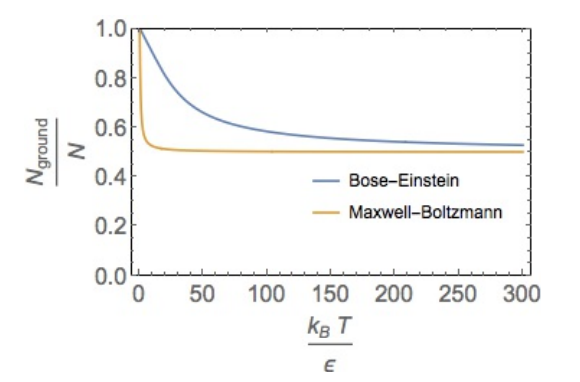
\includegraphics[width=0.75\textwidth]{images/BEC_1}
	\caption{From: MS's lecture notes.}
	\label{fig:1}
\end{figure}



\begin{framed}
	\begin{center}
		At which critical temperature $T_c$ does BEC occur?
	\end{center}
\end{framed}


To find $T_c$, we consider two limits: the high- and low-temperature limits, given by $k_bT/\epsilon \gg N \gg 1$ and $N\gg k_BT/\epsilon \gg 1$. We note that in both cases we want $N\gg 1$ because most real systems are large. The first limit is as expected:
\begin{equation*}
\f{\langle N_g^{BE}\rangle}{N} \approx \f{1}{2} + \f{N\epsilon}{12 k_B T} + \dots \to \f{1}{2} \quad \text{as } T\to \infty.
\end{equation*}
This is just the classical-behavior limit. In the second limit, we have
\begin{equation*}
\f{\langle N_g^{BE}\rangle}{N} \approx  1 - \f{k_BT}{N\epsilon} + \dots \to 1 \quad \text{as } T\to 0.
\end{equation*}
The comparison between these approximations and the exact expression is given in Figure \ref{fig:2}. The red line is the low-temperature limit; the green line is the high-temperature limit. The blue line is from the exact expression. 


\begin{figure}[!htb]
	\centering
	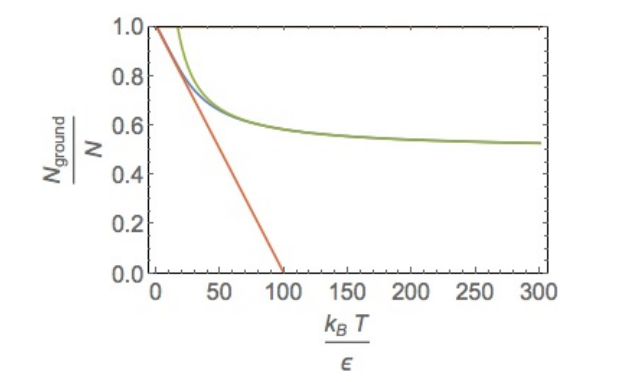
\includegraphics[width=0.75\textwidth]{images/BEC_2}
	\caption{From: MS's lecture notes.}
	\label{fig:2}
\end{figure}

The crossover points indicate when the expansions break down. In the first expansion, the second term is on the same order as the first term when $k_B T\approx N\epsilon/6$. In the second expansion, the second term is on the same order as the first term when $k_BT\approx N\epsilon$. So, the critical temperature $T_c$ is roughly $N\epsilon / k_B$ for the two-state model. \\


Now we will calculate $T_c$ for a more general case using the grand-canonical ensemble with chemical potential $\mu$. This simplifies the computation more than the approach using $N$ (for combinatorial reasons). \\


As we may know, for BE statistics, the expected number of particles in state $i$ (with energy $\epsilon_i$) is given by 
\begin{equation*}
\langle n_i \rangle = \f{1}{e^{-\be(\epsilon_i - \mu) - 1}}.
\end{equation*}
Thus, the expected number of particles in the ground state $\epsilon_0 = 0$ is 
\begin{equation*}
\langle N_g^{BE}\rangle = \f{1}{e^{-\beta u} -1}.
\end{equation*}
We see that $\mu$ must always be lower than all energies $\epsilon_i$ (which means that $\mu < 0$ since $\epsilon_0 = 0$). This is also why BEC only happens for the ground state.\\


Now, our goal is to solve for $\langle N_g^{BE}\rangle/N$. To start, we invert to solve for $\mu$:
\begin{equation*}
e^{-\beta \mu} = \f{1}{\langle N_g^{BE} \rangle} + 1.
\end{equation*}
Next, we want to relate $\langle N_g^{BE} \rangle$ to $N$ via 
\begin{equation*}
N = \sum_i \langle n_i \rangle  = \sum_i \f{1}{e^{\beta\epsilon_i} e^{-\be\mu} - 1} = \sum_i \f{1}{e^{\be\epsilon_i} \lp \f{1}{\langle N_g^{BE}\rangle} + 1 \rp - 1 }.
\end{equation*}
Once we fix some value for $\langle N_g^{BE}\rangle$ and have the $\epsilon_i$'s then it is possible to compute $N$ and thus find $\langle N_g^{BE}\rangle / N$. 


\subsection*{Numerical solution}

Consider non-relativistic gas in a box of side length $L$. The particles have wave number $\vec{k}_n = \pi \vec{n}/L$ with momenta $\vec{p} = \hbar \vec{k}$. The (kinetic) energies are just 
\begin{equation*}
\epsilon_n = \f{\hbar \vec{k}_n^2}{2m} = \f{\hbar^2 \pi^2 \vec{n}^2}{2mL^2}
\end{equation*}
which is the familiar particle-in-a-box energy. Here, 
\begin{equation*}
\vec{n}^2 = n_x^2 + n_y^2 + n_z^2.
\end{equation*}
Setting $\epsilon_0$, and we get the gap between the ground and first excited state (which is very important)
\begin{equation*}
\epsilon_n  = \f{\hbar^2 \pi^2 (1,0,0)^2 n^2}{2mL^2}  = \epsilon_1 n^2. 
\end{equation*} 
Plugging this into the previous expression for $N$, we have
\begin{equation*}
N = \sum^\infty_{n_x,n_y,n_z=0} \f{1}{e^{\beta \epsilon_1(n_x^2+n_y^2+n_z^2)} \lp \f{1}{\langle N_g^{BE}\rangle +1} \rp -1 }.
\end{equation*}
With this formula, we can compute $N$ given $\langle N_g^{BE}\rangle$ and $\beta \epsilon_1$. \\


What we really want, though, is to find $\langle N_g^{BE}\rangle $ as a function of $\beta$ given $\epsilon_1$ and $N$. We can't do this exactly, but we can make decent approximations in Mathematica. To do this, we need to do the sum and then solve for $\langle N_g^{BE}\rangle$ numerically. Figure \ref{fig:3} shows the solution for various (large) values of $N$. 


\begin{figure}[!htb]
	\centering
	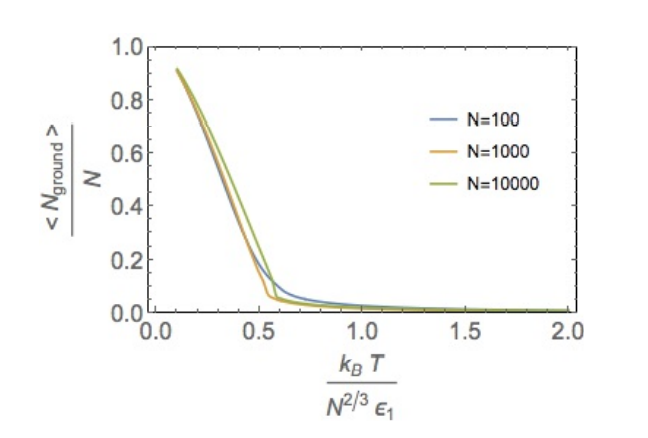
\includegraphics[width=0.75\textwidth]{images/BEC_3}
	\caption{From: MS's lecture notes.}
	\label{fig:3}
\end{figure}



For different $N$ the curve shifts, but looks qualitatively the same. It turns out that if we plot the ground state occupancy as a function of $k_BT /N^{2/3}\epsilon_1$ then the result is essentially independent of $N$ for BE statistics. 





\subsection*{Approximate analytical solution}

We want to convert sums into integrals. To do this, we follow this rule:
\begin{equation*}
\sum_{\vec{n}} \to \f{1}{8}\int^\infty_0 4\pi n^2\,dn.
\end{equation*}
Next we want to convert $n$ to $\epsilon$:
\begin{equation*}
\epsilon = \epsilon_1 n^2 \implies d\epsilon = 2\epsilon_1 n\,dn.
\end{equation*}
So,
\begin{equation*}
\sum_{\vec{n}} \to \dots = \f{\pi}{4\epsilon_1^{3/2}} \int^\infty_0 \sqrt{\epsilon}\,d\epsilon \equiv \int g(\epsilon)\,d\epsilon,
\end{equation*}
where $g(\epsilon)$ is the density of states. 


At this point, we would like to integrate over $\epsilon$ to find $N$:
\begin{equation*}
N = \int^\infty_0 g(\epsilon)\langle n_\epsilon\rangle \,d\epsilon = \f{\pi}{4\epsilon_1^{3/2}}\int^\infty_0 \,d\epsilon \sqrt{\epsilon} \f{1}{e^{\be(\epsilon-\mu)} - 1}
\end{equation*}
but this is not quite right. The integral only makes sense if we don't care about discreteness. For BEC, we have to care about discreteness because the ground state is qualitatively different from the rest. \\


Since the chemical potential $\mu$ can never approach any of the excited state energies (as it has an upper bound set by the ground state energy), the excited states' occupancy numbers will never be unusually large. Thus, we can just set $\mu  =0$ and let us proceed by taking the continuum limit for all but the ground state. With this, we find 
\begin{equation*}
\langle N_{\text{excited}} \rangle =  \f{\pi}{4\epsilon_1^{3/2}}\int^\infty_0 \,d\epsilon \sqrt{\epsilon} \f{1}{e^{\be(\epsilon-\mu)} - 1} = \lp \f{\pi k_B T}{4\epsilon_1} \rp^{3/2} \zeta_{3/2}
\end{equation*}
where $\zeta_{3/2} = \zeta(3/2) \approx 2.61$ with $\zeta$ being the Riemann zeta function. \\

The approximation $\mu=0$ breaks down when $N_g \to 0$, since $\mu \approx -k_B T \ln (N_g)\to -\infty$ as $N_g \to 0$. Thus, the approximation breaks down when $\langle N_{\text{excited}}\rangle \approx N$, i.e., it breaks down when 
\begin{equation*}
\langle N_{\text{excited}} \rangle =\lp \f{\pi k_B T}{4\epsilon_1} \rp^{3/2} \zeta_{3/2} > N.
\end{equation*} 
We can write this as $T>T_c$ where the \textbf{critical temperature} is defined by 
\begin{equation*}
{N = \lp \f{\pi k_B T_c}{4\epsilon_1} \rp^{3/2} \zeta_{3/2} = 2.612 \lp \f{mk_B T_c}{8\hbar^2 \pi} \rp^{3/2} V}
\end{equation*}
where we have used the previously given expression for $\epsilon_1$. So, $T_c$ is 
\begin{equation*}
\boxed{T_c = \f{4\epsilon_1}{\pi k_B} \lp \f{N}{\zeta_{3/2}} \rp^{2/3} = 3.31 \f{\hbar^2}{k_B m} \lp \f{N}{V} \rp^{2/3}  }
\end{equation*}


With this, we can write
\begin{equation*}
\f{N_\text{excited}}{N} = \lp \f{T}{T_c} \rp^{3/2}, \quad T < T_c
\end{equation*}
from which we find the fraction in the ground state: 
\begin{equation*}
\f{\langle N_g \rangle}{N} = 1-  \lp \f{T}{T_c} \rp^{3/2}.
\end{equation*}

Figure \ref{fig:4} shows the comparison between numerical calculations and the analytical approximation.

\begin{figure}[!htb]
	\centering
	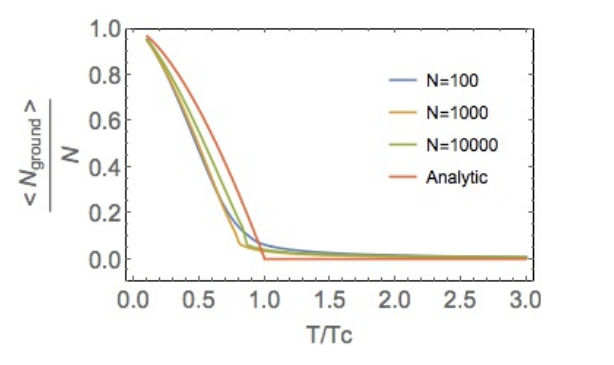
\includegraphics[width=0.75\textwidth]{images/BEC_4}
	\caption{From: MS's lecture notes.}
	\label{fig:4}
\end{figure}












%%%%%%%%%%%%%%%%%%%%%%%%%%%%%%%%%%%%%%%
\chapter*{C}
%%%%%%%%%%%%%%%%%%%%%%%%%%%%%%%%%%%%%%%
\chapter*{D}



\section*{Dark SPOT MOT}


%\section*{Dicke regime}



\section*{Doppler temperature}


Doppler temperature is the minimum temperature achievable with Doppler cooling. When an atom absorbs a counter-propagating photon, its velocity decreases due to momentum conservation. The atom then re-emits the photon (via spontaneous emission) in a random direction, giving the atom a momentum kick in a random direction. The random kicks average to zero, so the atom averages a zero mean velocity, i.e., $< v > = 0$. However, $<v^2> \neq 0$, so there is heat supplies to the atom. At equilibrium, the heating and cooling rates are equal; this is the limit on the amount by which the atom can be cooled using this technique. \\

If the transitions used for Doppler cooling have natural linewidths $\gamma$, then the Doppler temperature is given by 
\begin{equation*}
T_\text{Doppler} = \f{\hbar \gamma}{2k_B}
\end{equation*} 
where $k_B$ is the Boltzmann constant. This is usually much higher than the \textcolor{blue}{recoil temperature}, which is the temperature associated with the momentum gained from spontaneous emission. 






\section*{Dynamical System \& Feedback}



This section is mostly based on Sections II and III of \cite{bechhoefer2005feedback}. \\


Dynamical systems are often represented by some differential equation. A simple example is a \textbf{low-pass filter}, to which many sensors are equivalent. 

\begin{figure}[!htb]
	\centering
	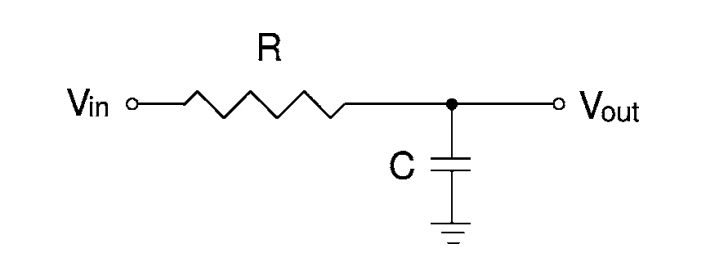
\includegraphics[width=0.5\textwidth]{images/low-pass-filter}
	\caption{From \cite{bechhoefer2005feedback}}
\end{figure}

Let the potentials be with respect to ground. By Kirchoff's law we have
\begin{equation*}
V_\text{out}(t) = \f{Q(t)}{C} = V_\text{in} - Ri(t) = V_\text{in} - R\dot{Q}(t) = V_\text{in} - RC\dot{V}_\text{out}.
\end{equation*}
So we have the following differential equation:
\begin{equation*}
\dot{V}_\text{out}(t) = -\f{1}{RC} V_\text{out}(t) + \f{1}{RC}V_\text{in}(t).
\end{equation*}


\begin{figure}[!htb]
	\centering
	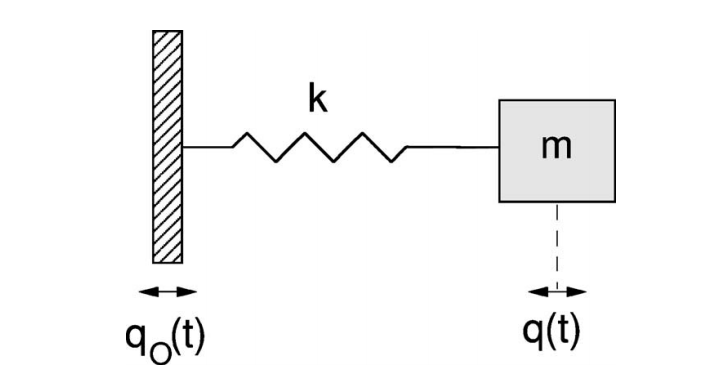
\includegraphics[width=0.5\textwidth]{images/DDHO}
	\caption{From \cite{bechhoefer2005feedback}}
\end{figure}



Another simple (and canonical) system is the damped driven harmonic oscillator:
\begin{equation*}
m\ddot{q} + 2\gamma \dot{q} + kq = k q_0(t).
\end{equation*}
Here, $\omega_0^2 = k/m$ is the natural resonance frequency, and we define $\zeta = \gamma/ \sqrt{mk}$ to be the damping parameter, with $0 <\zeta <1 $ for underdamping and $\zeta > 1$ for overdamping. With these, we have
\begin{equation*}
\ddot{q} + 2\zeta \dot{q} + q = q_0(t). 
\end{equation*}
From standard ODE theory, this second-order equation can be written as a system of two coupled first order ODEs. 


\subsection*{Laplace transform}


While thinking in time domain can be most natural, sometimes it is much more useful and intuitive to solve problems in control theory/dynamics systems in frequency domain. There two main tools for this purpose: Fourier transform and Laplace transform. In control theory, the Laplace transform has certain advantages over the Fourier transform since physical problems often have initial values that are more compatible with Laplace-transform methods. While the inverse Laplace transform is not as symmetric and ``nice'' as the Fourier transform, it is capable of transforming functions which do not decay to zero at infinity such as the Heaviside step function. Similarly, the Laplace transform can also handle unstable systems. The Laplace transform $y(s)$ of some signal $y(t)$ is given by 
\begin{equation*}
y(s) \equiv \lag[y(t)] = \int^\infty_0 y(t)e^{-ts}\,dt.
\end{equation*}
Two important identities of the Laplace transform are:
\begin{equation*}
\lag[d^n y(t)/dt^n] = s^n y(s) \quad \text{and} \quad \lag\lb \int y(t)\,dt \rb = \f{1}{s}y(s).
\end{equation*}
These identities are what make the Laplace transform useful: it transforms a differential equation into an algebraic equation. For example, Laplace-transforming the first-order equation
\begin{equation*}
\dot{y}(t) = -\omega_0 y(t) + \omega_0 u(t)
\end{equation*}
gives
\begin{equation*}
sy(s) = \omega_0 [ u(s) - y(s)],
\end{equation*}
which gives
\begin{equation*}
G(s) \equiv \f{y(s)}{u(s)} = \f{1}{1+ s/\omega_0}.
\end{equation*}

Here, $G(s)$ is called the \textbf{transfer function}, $u(s)$ is the driving function, i.e., the \textbf{input}, and $y(s)$ is the response, i.e., the \textbf{output}. The transfer function is the ratio of output to input (in frequency domain). In this particular example, $\omega_0 = 1/RC = 2\pi f_0$ is the characteristic angular frequency of the low-pass filter. \\

The \textbf{frequency response} of the system is a measure of the magnitude and phase of the output as a function of frequency, in comparison to the input. For example, if a sine wave is injected into a system at a certain frequency, a linear system will respond at that same frequency with a certain amplitude and phase relative to the input. Also, doubling the input amplitude also doubles the output amplitude. Thus, for linear (and time-invariant) systems, the frequency response can be seen as applying the system's transfer function to a purely imaginary number argument representing the frequency of the sinusoidal excitation. \\

In even simpler terms, by evaluating $G(s)$ at $s = i\omega$,  we have
\begin{equation*}
G(i\omega) = \f{y(i\omega)}{u(i\omega)}.
\end{equation*}
Now note that $y(i\omega)$ and $u(i\omega)$ are the Fourier transforms, i.e,. the \textbf{spectra}, of the output and input, respectively. This is what we mean by $G(i\omega)$ being the system's frequency response to the (spectrum) of the input. \\


In any case, back to our example, we have
\begin{equation*}
G(i\omega) = \f{1}{1 + i\omega/\omega_0}. 
\end{equation*}
From here, we can find the \textbf{amplitude} and \textbf{phase} of the frequency response $G(i\omega)$:
\begin{equation*}
\abs{G(i\omega)} = \f{1}{\sqrt{1+ \omega_0^2/\omega^2}} \quad \text{and} \quad \arg(G(i\omega)) = -\tan^{-1} \f{\omega}{\omega_0}.
\end{equation*}
So, the frequency response of a system is simply the transfer function obtained by the Fourier transform. 



\subsection*{Bode magnitude and phase plots}

The \textbf{Bode plot} for a linear, time-invariant system (which is what we're interested in most of the time -- so I will drop this condition from now on) with transfer function $G(s)$ consists of a magnitude and a phase plot.\\


The \textbf{Bode magnitude plot} is the log-log plot of $\abs{G(i\omega)}$ against $\omega$ (or $\omega_0$). Often, the magnitude is given in \textit{decibels}, i.e., the value being plotted is given by $20 \log_{10} \abs{G(i\omega)}$.  



\begin{figure}[!htb]
	\centering
	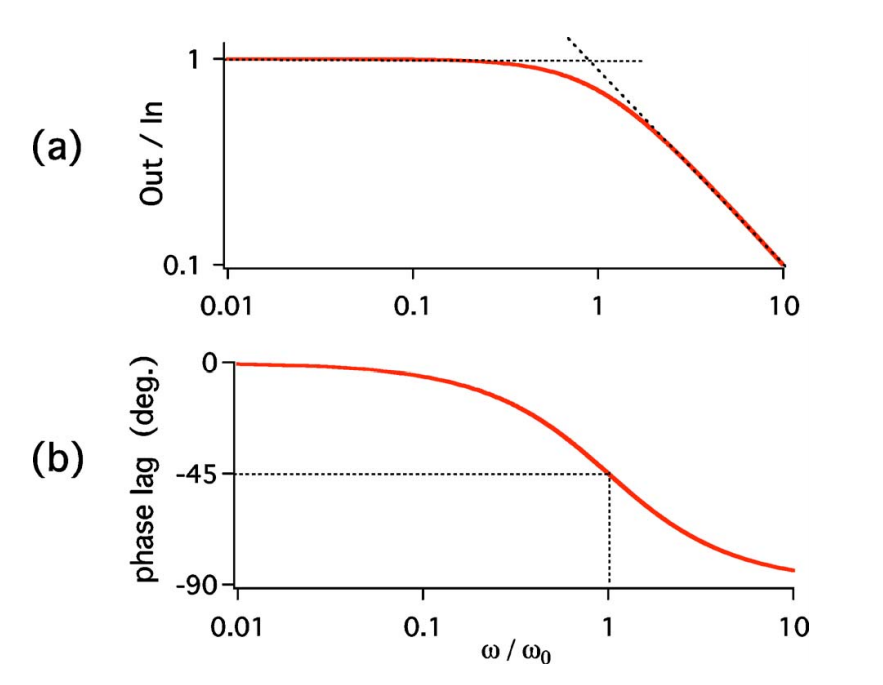
\includegraphics[width=0.7\textwidth]{images/bode-1st-order}
	\caption{From \cite{bechhoefer2005feedback}. Transfer function for a first-order, low pass filter. (a) Bode magnitude plot. The asymptotes intersect at the cutoff frequency $\omega_0$.  (b) Bode phase plot. The phase lag is $-\pi/2$ asymptotically, crossing $-\pi/4$ at $\omega_0$. }
\end{figure}




Similarly, the Laplace/Fourier transfer functions for the damped driven harmonic oscillator are 
\begin{equation*}
G(s) = \f{1}{1 + 2\zeta s + s^2} \quad \text{and}\quad G(i\omega) = \f{1}{1+ 2i\zeta\omega - \omega^2}.
\end{equation*}
With corresponding Bode plots:

\begin{figure}[!htb]
	\centering
	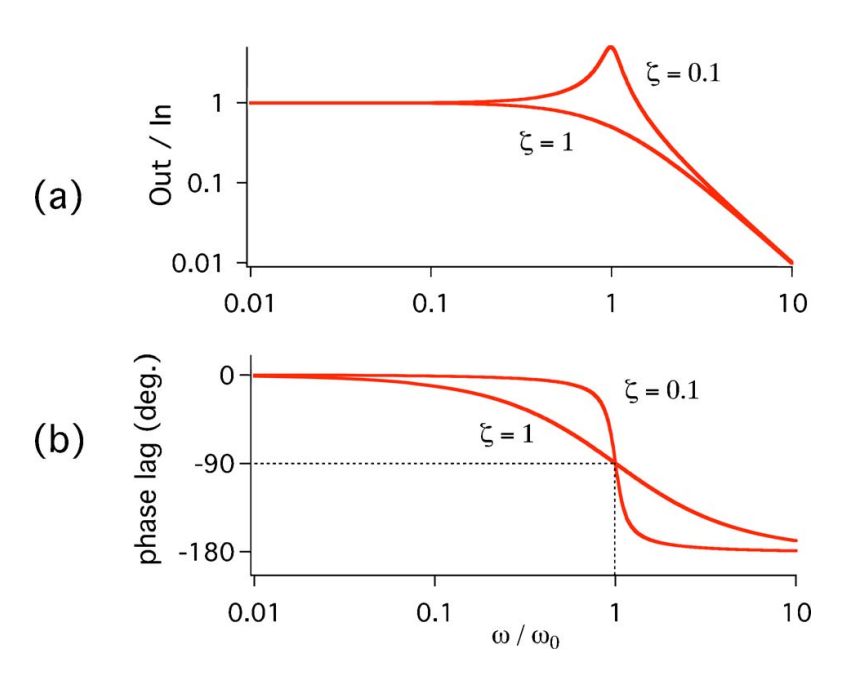
\includegraphics[width=0.7\textwidth]{images/bode-2nd-order}
	\caption{From \cite{bechhoefer2005feedback}. Transfer function for the damped driven harmonic oscillator. $\zeta = 1$ shows critically damped dynamics, while $\zeta = 0.1$ shows underdamped dynamics. (a) Bode magnitude plot.  (b) Bode phase plot. }
\end{figure}



\subsection*{Convolution theorem and transfer functions}


The convolution theorem says that
\begin{equation*}
\lag[G\ast H] = G(s)H(s),
\end{equation*} 
where $\ast$ denotes the convolution. This is not hard to prove and is left to the reader. \\


The convolution is needed when one wants to describe compound systems where the output of one element is fed into the input of the next element. Consider the following example. Suppose we have a damped driven harmonic oscillator as before: 
\begin{equation*}
\ddot{y} + 2\zeta \dot{y} + y = u(t)
\end{equation*}
with a first-order sensor which reports the position of the oscillator:
\begin{equation*}
\dot{v} + v = y(t). 
\end{equation*}
Here, we see that $u(t)$ drives the oscillator $y(t)$, and $y(t)$ drives the sensor output $v(t)$. Laplace transforming both equations gives
\begin{equation*}
y(s) = G(s)u(s) = \f{1}{1 + 2\zeta s + s^2}u(s) \quad \text{and} \quad v(s) = H(s)y(s) = \f{1}{1+s} y(s),
\end{equation*}
and so $v(s) = H(s) G(s) u(s) \equiv F(s) u(s)$. We see that having two elements in series leads to a transfer function that is the product
of the transfer functions of the individual elements. This motivates the block diagram below. We note that in time domain, the products become convolution products. 


\begin{figure}[!htb]
	\centering
	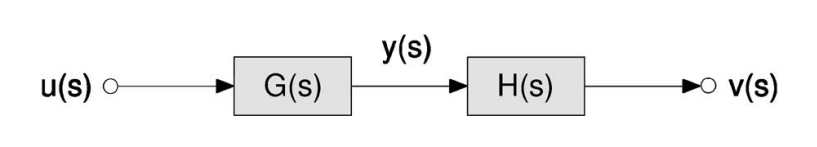
\includegraphics[width=0.75\textwidth]{images/block-1}
	\caption{From \cite{bechhoefer2005feedback}}
\end{figure}


\subsection*{Feedback}


Let some system be given whose dynamics is given by $G(s)$. Let the output be $y(t)$. Our goal is to make $y(t)$ follow some \textbf{control signal} $r(t)$ as faithfully as possible. To do this, we measure the \textbf{error signal} $e(t) = r(t) - y(t)$. We now apply some control law $K$ such that $\abs{e(t)}$ or $a\abs{e(t)}^2$ is minimized. The entire feedback system can be represented by the following block diagram:

\begin{figure}[!htb]
	\centering
	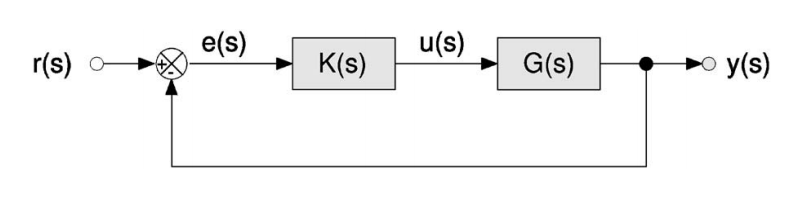
\includegraphics[width=0.75\textwidth]{images/block-2}
	\caption{From \cite{bechhoefer2005feedback}.}
\end{figure}

We ask what the relationship between the control signal and output signal is. To work this out, we first look at the top line. The error signal is used to generate the output signal. This relationship is 
\begin{equation*}
y(s) = G(s)K(s) e(s). 
\end{equation*}
Now, to the bottom line. The output is fed back into the system to generate a new error signal. We have $e(s) = r(s) - y(s)$, so 
\begin{align*}
y(s) = G(s)K(s) e(s) = G(s)K(s) [r(s) - y(s)] \\\implies y(s) = \f{K(s)G(s)}{1 + K(s)G(s)}r(s) \equiv \f{L(s)}{1 + L(s)}r(s) \equiv T(s) r(s). 
\end{align*}

Consider the low pass filter again, but this time with a DC gain $G_0$
\begin{equation*}
G(s) = \f{G_0}{1+ s/\omega_0},
\end{equation*}
and proportional feedback control law $K(s) = K_p$, a constant. Then, we have
\begin{equation*}
T(s) = \f{K_p G_0}{K_p G_0 + 1 + s/\omega_0} = \f{K_p G_0}{K_p G_0 +1} \f{1}{1 + s/[\omega_0(1 + K_p G_0)]}
\end{equation*}
This is nothing but a low pass filter once again, with modified gain and cutoff frequency. The new DC gain is of course $K_p G_0 / (1 + K_p G_0)$, and the new cutoff frequency is $\omega_0(1 + K_p G_0)$. \\


Next, we consider the effects of an output disturbance $d(t)$ and sensor noise $\xi(t)$. The corresponding block diagram is now
\begin{figure}[!htb]
	\centering
	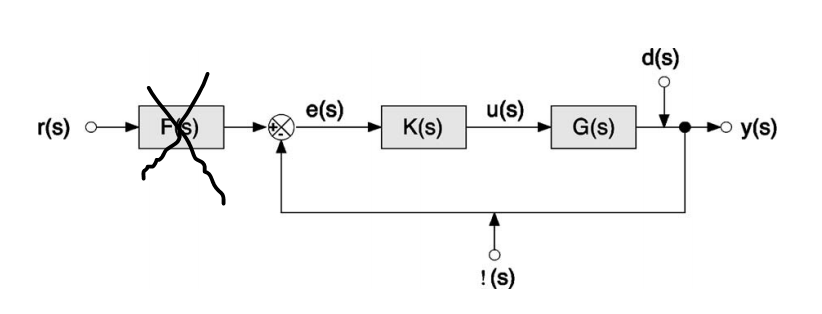
\includegraphics[width=0.75\textwidth]{images/block-3}
	\caption{From \cite{bechhoefer2005feedback}.}
\end{figure}
Here, we have
\begin{equation*}
e(s) = r(s) - [y(s) + \xi(s)] = r(s) - y(s) - \xi(s) 
\end{equation*}
and
\begin{equation*}
y(s) = G(s) K(s) e(s) + d(s).
\end{equation*}
From here, we find 
\begin{equation*}
y(s) = \f{KG}{1+KG}[r(s) - \xi(s)] + \f{1}{1+ KG}d(s). 
\end{equation*}

Assuming that we're still working with a low pass filter, we make a few remarks:
\begin{itemize}
	\item The disturbances $d(t)$ would have been rejected up to cutoff frequency $\omega' = \omega_0(1+ K_p G_0)$. This is a good thing. 
	
	\item The control signal effectively becomes $r-\xi$, and the system has no way to distinguish the control signal from the measurement noise $\xi(t)$. This means that the higher the gain is (recall that the gain is $KG/(1+KG)$), the noisier the output. 
\end{itemize}


The frequency $\omega'$ is called the \textbf{feedback bandwidth}. From our analysis we see that high feedback bandwidth is \textbf{good} because it allows the system to track rapidly varying control, but also \textbf{bad} because it also noise through which contaminates the output. This tradeoff can be express by rewriting the equation above as 
\begin{align*}
e_0(s) \equiv r(s) - y(s) &= r(s) - \lb \f{KG}{1+KG}[r(s) - \xi(s)] + \f{1}{1+ KG}d(s)  \rb \\
&= \f{1}{1+KG}[r(s) - d(s)] + \f{KG}{1+KG}\xi(s) \\
&\equiv S(s)[r(s) - d(s)] + T(s) \xi(s). 
\end{align*}
Here, we call $e_0(s)$ the \textbf{tracking error signal}, $S(s)$ the \textbf{sensitivity function} and $T(s) = 1- S(s)$ the \textbf{complementary sensitivity function}. The goal is to minimize $e_0$, of course. However, a fundamental obstacle is that $S+T = 1$ at all frequencies: if $S$ is small and disturbances are rejected then the output becomes noisy, and vice versa. There are ways around this, though. 


\subsection*{Feedforward}


Wikipedia has a nice explanation for \textbf{feedforward} so I'll just paste it here: ``With feed-forward or feedforward control, the disturbances are measured and accounted for before they have time to affect the system. In the house example, a feed-forward system may measure the fact that the door is opened and automatically turn on the heater before the house can get too cold. The difficulty with feed-forward control is that the effects of the disturbances on the system must be accurately predicted, and there must not be any unmeasured disturbances. For instance, if a window was opened that was not being measured, the feed-forward-controlled thermostat might let the house cool down.'' \\


To implement this, one may apply a \textbf{prefilter} $F(s)$ to the control signal $r(s)$. In the absence of any feedback, the system response is just $y(s) = F(s)G(s)r(s)$. If we can choose $F = G^{-1}$ then $y$ just follows $r$ directly, which is what we mean by ``feedforward.'' In practice, it is impossible to find $F = G^{-1}$; however, one can approximate $G^{-1}$. \\


Since it is not possible to implement feedforward and because disturbances are usually unknown, in practice one usually combines feedforward with feedback. A block diagram for this scheme has the form

\begin{figure}[!htb]
	\centering
	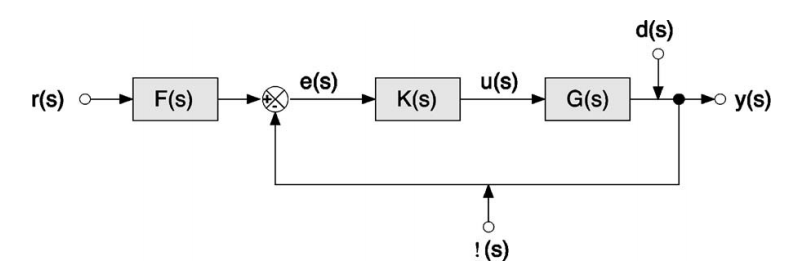
\includegraphics[width=0.75\textwidth]{images/block-4}
	\caption{From \cite{bechhoefer2005feedback}}
\end{figure}

The output now becomes
\begin{equation*}
y(s) = \f{KG}{1+KG}[F(s)r(s) - \xi(s) ] + \f{1}{1+KG}d(s).
\end{equation*}

Choose $F$ as close as possible to $1+(KG)^{-1}$ reduces the load on the feedback while simultaneously rejecting disturbances via the feedback loop. 


\subsection*{Case study: Operational Amplifier (OpAmp)}


An op amp is basically a very high gain differential amplifier that uses negative feedback to trade off high gain for reduced sensitivity to drift. 

\begin{figure}[!htb]
	\centering
	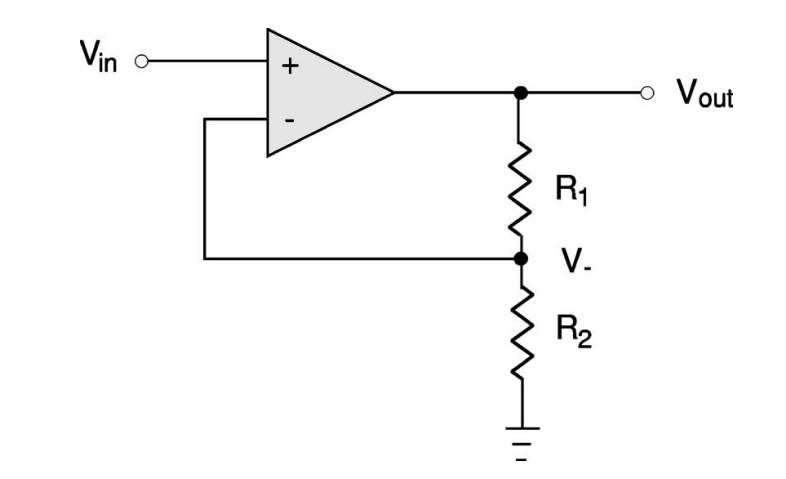
\includegraphics[width=0.75\textwidth]{images/op-amp}
	\caption{From \cite{bechhoefer2005feedback}}
\end{figure}

The op amp in the configuration above does the following:
\begin{equation*}
V_\text{out} = A(V_\text{in} - V_-),
\end{equation*}
where $A$ is the gain. We want to find the transfer function $G$ which is also the closed-loop gain. The resistors $R_1$ and $R_2$ form a voltage divider:
\begin{equation*}
V_- = V_\text{out} \f{R_2}{R_1 + R_2} \equiv V_\text{out} \beta.
\end{equation*}
From here, we can find 
\begin{equation*}
G = \f{V_\text{out}}{V_\text{in}} = A - A\f{V_-}{V_\text{in}} = A - A\f{V_\text{out}}{V_\text{in}} \beta \implies G = \f{V_\text{out}}{V_\text{in}} = \f{A}{1+A\beta}. 
\end{equation*}
When $A \gg 1$, we have an approximation:
\begin{equation*}
G \approx \f{1}{\beta} = \f{R_1 + R_2}{R_2} = 1 + \f{R_1}{R_2}. 
\end{equation*}








\subsection*{Integral control}

So far, we have only covered proportional control, which suffers from \textbf{proportional droop} -- meaning that there is always some non-zero difference between the set point and the output of the system: only for an infinite gain that $y_\infty = r_\infty$. \\


In integral control, one applies a control $K_i \int_{-\infty}^t e(t')\,dt'$ instead of (just) the proportional term $K_p e(t)$. As long as $e(t) \neq 0$, the integral will build up and eliminates steady state error. This can be seen in the time domain:
\begin{equation*}
\dot{y}(t) = -\omega_0 y(t) + \omega_0^2 K_i \int_{-\infty}^t [r_\infty - y(t')]\,dt'
\end{equation*} 
which after differentiating gives
\begin{equation*}
\ddot{y}(t) = -\omega_0\dot{y}(t) + \omega_0^2 K_i [r_\infty - y(t)]
\end{equation*}
which has steady state solution $y_\infty = r_\infty$. Now we want to go into frequency domain. To do this, we first recall that $y(s) = K(s) G(s) e(s)$. To find $K(s)$, we Laplace-transform $K(t)$, which requires the identity $\lag[\int e(t)\,dt] = e(s)/s$:
\begin{equation*}
K(s) = \lag[K(t)] = K_i \f{e(s)}{s}.
\end{equation*}
So,
\begin{equation*}
\dot{y}(s) = -\omega_0 \lb y(s) + \f{K_i}{s/\omega_0} \rb e(s).
\end{equation*}
Consider the low pass filter again with transfer function 
\begin{equation*}
G(s) = \f{1}{1+ s/\omega_0}.
\end{equation*}
With this $K(s)$, the complementary sensitivity function becomes
\begin{equation*}
T(s) = \f{KG}{1+ KG} = \f{1}{1 + \f{s}{\omega_0 K_i} + \f{s^2}{K_i \omega_0^2}}.
\end{equation*}
We see that this new transfer function resembles a second-order system. Indeed, the integral control law transform a first-order system into a second-order system, with new natural frequency ${\omega_0'}^2 = K_i \omega_0^2$ and $\zeta = 1/2\sqrt{K_i}$. \\


Integral control can be improved by combining with proportional control:
\begin{equation*}
K(s)  = K_p + \f{K_i}{s/\omega_0},
\end{equation*}
which gives faster response while still eliminating steady-state errors. One can write down the closed-loop transfer function and show that $T\to 1$ for $\omega\to 0$ and is asymptotically first-order with time constant $1/K_p \omega_0$. \\


In general, the transfer function for a PID controller is given by 
\begin{equation*}
K(s) = K_p + \f{K_i}{s} + K_d s.
\end{equation*}
In a closed-loop system with transfer function $G(s)$ without any noise or measurement error, the overall transfer function is given by 
\begin{equation*}
T(s) = \f{K(s)G(s)}{1+ K(s)G(s)}. 
\end{equation*}
Adding noise and measurement error follows the same procedure as described above. 








%%%%%%%%%%%%%%%%%%%%%%%%%%%%%%%%%%%%%%%
\chapter*{E}



\section*{Electromagnetically induced transparency (EIT)}



%%%%%%%%%%%%%%%%%%%%%%%%%%%%%%%%%%%%%%%
\chapter*{F}


\section*{Feshbach Resonance (in ultracold gases)}


To start, let us look at some results in scattering theory. For more information about this topic, the reader may refer to \cite{sakurai1995modern}. Consider a general wave-scattering problem where we have an incident plane wave with wave number $k$ and a radial scattered wave with anisotropy term (partial wve scattering amplitude) $f(\theta)$: 
\begin{equation*}
\phi_\text{inc} = e^{ikz}, \quad \phi_{\text{sc}} = \f{f(\theta)e^{ikr}}{r}
\end{equation*}
and by definition
\begin{equation*}
d\sigma = \abs{f(\theta)}^2\, d\Omega.
\end{equation*}
Consider a particle of mass $m$, energy $\hbar^2k^2/2m$, in a central potential $V(r)$. At large $r$, the wave function is approximated by the sum of the waves above:
\begin{equation*}
\phi_{\text{large } r} = \phi_{\text{inc}} + \phi_{\text{sc}}. 
\end{equation*}
Since $\phi_{\text{large } r}$ must also solve the SE, which is separable due to $V(r)$ being central, we have \cite{bohm2012quantum}
\begin{equation*}
\phi_{\text{large } r} = Y(\theta)R(r) = \lp \sum^\infty_{l=0} C_l P_l(\cos\theta) \rp \f{1}{kr}\sin\lp kr - \f{l\pi}{2} + \delta_l \rp
\end{equation*}
By re-writing $\phi_\text{large $r$}$ like this we find 
\begin{equation*}
f(\theta) = \f{1}{k}\sum^\infty_{l=0} \sin \delta_l P_l(\cos\theta).
\end{equation*}
Here $l$, the angular momentum quantum number, corresponds to different partial waves. \\

Now recall the radial SE:
\begin{equation*}
-\f{\hbar^2}{2m}\f{d^2 u(r)}{dr^2} + V_\text{eff}(r)u(r) = Eu(r)
\end{equation*} 
where
\begin{equation*}
V_\text{eff}(r) = V(r) + \f{\hbar^2l(l+1)}{2mr^2}.
\end{equation*}
The form of $V_\text{eff}$ implies that the particles cannot reach small $r$'s for $l>0$. So, by assuming that $V(r)$ is only significant/nontrivial for small $r$, we find that only $l=0$ matters. So, we only care about $s$-waves in the expansion. With this, we have
\begin{equation*}
\phi_{\text{large } r} = \f{C_0}{kr} \sin(kr - \delta_0) = 
\end{equation*}
This means that
\begin{equation*}
f = -\f{1}{k}e^{i\delta_0 }\sin\delta_0 = \f{1}{k\cot\delta_0 -ik}. 
\end{equation*}

The \textcolor{blue}{$s$-wave scattering length} $a$ is defined as 
\begin{equation*}
a = -\lim_{k\to 0}\f{\tan \delta_0 (k)}{k}
\end{equation*}
\begin{itemize}
	\item For strong and attractive interactions, $a$ is large and negative
	
	\item For strong and repulsive interactions, $a$ is large and positive. 
\end{itemize}
By Taylor expansion we have
\begin{equation*}
k\cos(\delta_0(k)) \approx -\f{1}{a} + \f{1}{2}r_\text{eff} k^2 + \dots
\end{equation*}
where $r_\text{eff}$ is the effective range of the potential. Plugging this back into the equation for $f$ we find 
\begin{equation*}
f(k) = \f{1}{-1/a + r_\text{eff} k^2/2 - ik}.
\end{equation*}
From the Lippmann-Schwinger equation for $s$-waves, we find that 
\begin{equation*}
\f{1}{f(k)} \approx -\f{4\pi}{v_0} + \f{4\pi}{v_0} \int\f{d^3q}{(2\pi)^3} \f{v(\mathbf{q})}{k^2 - q^2 - i\eta}
\end{equation*}
where $v(\cdot)$ is the interatomic potential. \\


Now let us apply some of this to ultracold Fermi gases. Consider two Fermionic atoms in close proximity. The effective interaction between them depends on the angular momentum coupling of their valence electrons, $\ket{s_1,m_1}\otimes \ket{s_2,m_2}$, where $s$ is the total spin quantum number and $m$ is the spin projection quantum number. The valance electrons can be in the singlet or one of the triplet state. If the electrons are in the singlet state with antisymmetric spin wave function 
\begin{equation*}
\ket{0,0} = \f{1}{\sqrt{2}}\lp \ket{\uparrow\downarrow} - \ket{\downarrow \uparrow} \rp
\end{equation*}
then they must have symmetric spatial wave function (since they are fermions -- the total wavefunction must be anti-symmetric), and so they can exist close together. On the other hand, if the spin wave function is one of the triplet states (which are symmetric) 
\begin{equation*}
\ket{1,1} = \ket{\uparrow\uparrow}, \ket{1,0} = \f{1}{\sqrt{2}} \lp \ket{\uparrow\downarrow} + \ket{\downarrow\uparrow} \rp, \text{ or } \ket{1,-1} = \ket{\downarrow\downarrow}
\end{equation*}
then the spatial wave function is anti-symmetric, and thus they cannot be close to each other. \\


As a result, the singlet interatomic potential $V_S$ is deeper than the triplet potential $V_T$. For simplicity, we assume that $V_S$ is just deep enough to contain only one bound state and that $V_T$ contains no bound states.\\


In addition to the interaction potential, there is also the hyperfine interaction
\begin{equation*}
V_\text{hf} = \f{\al}{\hbar^2} \mathbf{I}\cdot \mathbf{S}
\end{equation*}
and the Zeeman shift $\Delta \mu B$ between the singlet and triplet states (which are degenerate), where $\Delta \mu$ is the difference in magnetic moments between the two states. We assume that $0< V_\text{hf} \ll V_T,V_S,\Delta \mu B$. 


\subsection*{Example: Spherical well model}







%\section*{Free spectral range (FSR)}


%%%%%%%%%%%%%%%%%%%%%%%%%%%%%%%%%%%%%%%
\chapter*{G}


\section*{Gross-Pitaevskii equation and BEC}

In this section we derive the Gross-Pitaevskii equation (GPE) which describes the dynamics of BECs. The derivation presented in this section is provided by \cite{rogel2013gross}. 


A BEC is obtained from a collection
of bosons in the ground state at very low temperatures. We can therefore ask about
the energy of the ground state and use this to provide us with information about the
system. The general Hamiltonian for an $N$ particle system is given by 
\begin{equation*}
\ham = \sum^N_{i=1} \lp \f{\mathbf{p}_i^2}{2m} + V_{ext}(\mathbf{r}_i) \rp + \f{1}{2}\sum^N_{i=1}\sum^N_{j\neq i}V\lp \abs{\mathbf{r}_i - \mathbf{r}_j} \rp
\end{equation*}

The first term is the KE of the $i$-th particle, followed by the trapping potential. The final term is represents the interaction energy between the $N$ particles. The ground state corresponds to the lowest energy and we can find it by minimizing the energy associated with this Hamiltonian. From the thermodynamics point of view, the ground state of the system is achieved when the \textbf{free energy} $F = E - \mu N$ is minimized. Here, $E$ is the energy of the system, and $\mu$ is the chemical potential. \\


Given $\ham$, the energy is just the expectation value of $\ham$:
\begin{equation*}
E(\psi) = \f{\bra{\psi} \ham \ket{\psi}}{\braket{\psi}}. 
\end{equation*}

We will use this to minimize $F$. Now, every particle in the system has some wavefunction $\psi_i$. But solve a problem exactly with $N$ such $\psi_i$'s is very difficult: if there are $N$ particles then there are $N^2$ terms in the Hamiltonian. So, to simplify the problem, we resort to making the \textbf{mean-field approximation}, which basically says that the action felt by a given particle due to the rest is substituted by the mean action of the fluid over the particle. The mean-field approximation is good if one can neglect the corresponds in the gas, i.e., if the gas is \textbf{dilute}, which turns out to be the case for experimentally obtained condensates. The approximation fails if closer neighbors interact too much strongly compared to particles further apart. \\


In any case, under the mean-field approximation, or one particle, all the rest have the same status as they all are in the same independent state $\ket{\psi}$ and thus we can drop the label of wavefunctions. Thus, we need to minimize the free energy over a space of functions given by 
\begin{equation*}
\ket{\Psi} = \otimes \ket{\psi}
\end{equation*}
with the normalization condition
\begin{equation*}
\braket{\Psi} = 1.
\end{equation*}

With this, we want to minimize
\begin{equation*}
F(\Psi) = \bra{\Psi} \ham \ket{\Psi} - \mu \braket{\Psi}.
\end{equation*}
We now compute each term:
\begin{align*}
\bra{\Psi}  \sum^N_{i=1} \f{\mathbf{p}_i^2}{2m}  \ket{\Psi} 
&= \sum^N_{i=1}\f{\hbar^2}{2m} \int \nabla \psi^*(\mathbf{r}_i) \nabla \psi(\mathbf{r}_i) \,d\mathbf{r}_i \\
&=  N\f{\hbar^2}{2m} \int \abs{\nabla \psi(\mathbf{r})}^2 \,d\mathbf{r}\\
&= -N \f{\hbar^2}{2m}\int \psi^*(\mathbf{r})\nabla^2 \psi(\mathbf{r})\,d\mathbf{r}.
\end{align*}
The potential term is written as 
\begin{align*}
\bra{\Psi} \sum^N_{i=1}V_{ext}(\mathbf{r}_i) \ket{\Psi} = N \int \psi^*(\mathbf{r}) V_{ext}(\mathbf{r}) \psi(\mathbf{r})\,d\mathbf{r}.
\end{align*}
Interaction energy term:
\begin{align*}
\bra{\Psi} \f{1}{2}\sum^N_{i=1}\sum^N_{j\neq i} V(\abs{\mathbf{r}_i - \mathbf{r}_j}) \ket{\Psi} 
&= \f{1}{2}\sum^N_{i=1}\sum^N_{j\neq i} \int \,d\mathbf{r}_i \int \,d\mathbf{r}_j \psi^*(\mathbf{r}_i) \psi^*(\mathbf{r}_j) V(\abs{\mathbf{r}_i - \mathbf{r}_j}) \psi(\mathbf{r}_i) \psi(\mathbf{r}_j) \\
&= \f{N(N-1)}{2} \int \,d\mathbf{r} \int \,d\mathbf{r}' \psi^*(\mathbf{r}_i) \psi^*(\mathbf{r}') V(\abs{\mathbf{r} - \mathbf{r}}) \psi(\mathbf{r}') \psi(\mathbf{r}').
\end{align*}
Finally the chemical potential term:
\begin{align*}
\mu \braket{\Psi} = \mu \lp \int \psi^*(\mathbf{r}) \psi(\mathbf{r}) \,d\mathbf{r} \rp^N.
\end{align*}

Now we want to minimize $F$. We do this using calculus of variations. We will consider small variations in $\psi(\mathbf{r}$, taking $\psi$ and $\psi^*$ as independent variables. Finding $\delta/\delta \psi$ and $\delta/\delta \psi^*$ for the expressions containing the kinetic and potential terms is rather straightforward. For the interaction term, we have
\begin{equation*}
\f{\delta}{\delta \psi^*} \bra{\Psi} \f{1}{2}\sum^N_{i=1}\sum^N_{j\neq i} V(\abs{\mathbf{r}_i - \mathbf{r}_j}) \ket{\Psi} \\
= N(N-1) \int \delta \psi^*(\mathbf{r}) \lp \int \abs{\psi(\mathbf{r})}^2 V(\abs{\mathbf{r} - \mathbf{r}'}) \,d\mathbf{r}' \rp \psi(\mathbf{r})\,d\mathbf{r}
\end{equation*}
Similarly, for the chemical potential we have
\begin{align*}
\f{\delta \braket{\Psi}}{\delta \psi^*}  &= N\lp \int \psi^*(\mathbf{r})\psi(\mathbf{r})\,d\mathbf{r} \rp^{N-1}\int \delta \psi^*(\mathbf{r}) \psi(\mathbf{r})\,d\mathbf{r} \\
&=  N\int \delta \psi^*(\mathbf{r}) \psi(\mathbf{r})\,d\mathbf{r}.
\end{align*}
Putting it together we have
\begin{equation*}
0=\f{\delta F}{\delta \psi^*} = N\int \lb  \f{-\hbar^2\nabla^2}{2m}  + V_{ext}(\mathbf{r})+ (N-1)\lp \int \abs{\psi(\mathbf{r})}^2V(\abs{\mathbf{r} - \mathbf{r}'})\,d\mathbf{r}' \rp  - \mu   \rb \psi(\mathbf{r}) \delta \psi^*(\mathbf{r})\,d\mathbf{r}.
\end{equation*}
So the term in the square bracket acting on $\psi$ must vanish. \\


It is common to choose an interaction potential
\begin{equation*}
V(\abs{\mathbf{r} - \mathbf{r}'}) = \f{4\pi \hbar^2}{m}a\delta(\mathbf{r} - \mathbf{r}')
\end{equation*}
where $a$ is the $s$-wave scattering length. Using the approximation that $N-1\approx N$ we have the \textbf{time-independent Gross-Pitaevskii equation}
\begin{equation*}
\boxed{\lp \f{-\hbar^2\nabla^2}{2m}  + V_{ext}(\mathbf{r})+ N \f{4\pi\hbar^2}{m}a\abs{\psi(\mathbf{r})}^2 \rp \psi(\mathbf{r})   = \mu \psi(\mathbf{r})}
\end{equation*}

The scattering length a
measures the intensity of the interactions between the bosons. Its sign indicates whether the interactions are attractive $(a < 0)$ or repulsive $(a > 0)$.


\subsection*{Remarks}

\noindent \textbf{Normalization:} While we can choose the normalization condition $\braket{\Psi} = 1$ so that it is the probability density of finding a boson, we can choose $\braket{\Psi} = N$, the square modulus of the number density of the fluid. \\

\noindent \textbf{Phase:} The phase doesn't have intrinsic meaning but its fluctuations do. Suppose we put the wavefunction is polar form:
\begin{equation*}
\psi = \sqrt{\rho} \exp(i\theta)
\end{equation*}
where $\theta$ is the phase and $\rho$ is the number density, then the probability current can be expressed as 
\begin{equation*}
\mathbf{j} = \f{i\hbar}{2m} \lp \psi \nabla \psi^* - \psi^* \nabla \psi \rp = \rho \f{\hbar }{m} \nabla \theta \equiv \rho \mathbf{v}.
\end{equation*}
Here
\begin{equation*}
\mathbf{v} = \f{i\hbar}{2m} \f{(\psi \nabla \psi^* - \psi^*\nabla \psi )}{\abs{\psi}^2}  =\f{\hbar}{m}\nabla \theta
\end{equation*}
is the velocity of the bosons. This expression will make better sense when we talk about the hydrodynamic form of the GPE.\\


\noindent \textbf{Trapping potential:}  Most of the time, the bosons are confined in a
small region of space (by optical and/or magnetic means). This situation is simulated with the aid of a trapping potential with a minimum in the central part. In general, any ``nice'' potential can be locally approximated by a harmonic potential with the condensate sitting in a position where the quadratic term is dominant:
\begin{equation*}
V_{ext}(\mathbf{r}) = \f{1}{2}m\omega^2 r^2.
\end{equation*}
Here $m$ is the mass of the bosons, and $\omega$ is the frequency of the trap. If atoms in the condensate do not interact (repulsive condensate, which is the case of 87Rb), then the ground state of the trapping potential on its own would just be a Gaussian $\psi(\mathbf{r})\propto e^{-(r/r_0)^2}$ where $r_0 \sim \sqrt{\hbar/m\omega} \approx 1.04 \mu$. However, experimentally formed condensates have parabolic form. This is because of the relatively large density. In this case, the kinetic energy is negligible compared to the rest of the terms, and we have
\begin{equation*}
\psi(\mathbf{r}) = \sqrt{\f{\mu - m\omega^2 r^2/2}{gN}}
\end{equation*}
which has parabolic form. This approximation is known as the \textbf{Thomas-Fermi approximation}. 


\subsection*{Time-dependent GPE}

The time-dependent GPE is given by 
\begin{equation*}
i\hbar \f{\p\psi}{\p t} = \lp -\f{\hbar^2}{2m} \nabla^2 + V_{ext} + g\abs{\psi}^2 \rp \psi
\end{equation*}
which we can see is a nonlinear SE. Let $\widetilde{\psi}$ be a solution using the normalization condition that $\braket{\widetilde{\psi}} = N(\widetilde{\psi})$. Multiplying both sides by $\widetilde{\psi}^*$ we have
\begin{equation*}
i\hbar [\p_t \widetilde{\psi}] \widetilde{\psi}^* = -\f{\hbar^2}{2m} [\nabla^2 \widetilde{\psi} ] \widetilde{\psi}^* + V_{ext} \abs{\widetilde{\psi}}^2 + g \abs{\widetilde{\psi}}^4.
\end{equation*}
Writing a similar equation for $\widetilde{\psi}^*$ and adding the two equations together, we find 
\begin{equation*}
2i\p_t N(\widetilde{\psi}) = \int d^3 \mathbf{r} \lb -\f{\hbar^2}{2m} \abs{\nabla \widetilde{\psi}}^2 + V_{ext}(\mathbf{r}) \abs{\widetilde{\psi}}^2 + \f{g}{2} \abs{\widetilde{\psi}}^4 \rb - \mu \abs{\widetilde{\psi}}^2.
\end{equation*}

Notice the LHS is purely imaginary since $N$ is real, so the quantity
\begin{equation*}
E \equiv \int d^3 \mathbf{r} \lb -\f{\hbar^2}{2m} \abs{\nabla \widetilde{\psi}}^2 + V_{ext}(\mathbf{r}) \abs{\widetilde{\psi}}^2 + \f{g}{2} \abs{\widetilde{\psi}}^4 \rb,
\end{equation*}
which corresponds to the total energy of the bosonic gas, must be conserved. So, we see that the solution to GPE has \textbf{two} conserved quantities: the number of particles $N$ and the energy $E$ of the system. 


\subsection*{Hydrodynamic form of the GPE}

Here we introduce the hydrodynamic form of the GPE, which is equivalent to the time-dependent GPE. As pointed out earlier, for a solution $\psi = \sqrt{\rho} \exp(i\theta)$, one can use the density $\rho$ and gradient of the phase $\nabla \theta$ to work out the dynamics of the system.\\


The first hydrodynamic equation is the \textbf{continuity equation}: 
\begin{equation*}
\f{\p \rho}{\p t} + \nabla \cdot \mathbf{j} = 0.
\end{equation*}
This holds for the GPE problem because we can derive this equation from the GPE by multiplying it by $\psi^*$ and subtracting the c.c. of the resulting equation. Now, recall that 
\begin{equation*}
\mathbf{j} = \f{i\hbar}{2m}\lp \psi \nabla \psi^* - \psi^* \nabla \psi \rp = \rho \mathbf{v} \equiv \rho\f{\hbar}{m}\nabla \theta.
\end{equation*}
So the continuity equation becomes
\begin{equation*}
\boxed{\f{\p \rho}{\p t}  + \nabla \cdot (\rho \mathbf{v}) = 0}
\end{equation*}
This says that the motion of the condensate corresponds to that of a flow since the velocity field $\mathbf{v}$ is a gradient of a scalar quantity $\theta$. Also, if the phase $\theta$ is not singular, then the velocity field is conservative, or \textbf{irrotational}.
\begin{equation*}
\nabla \times \mathbf{v} \sim \nabla \times \nabla \theta = 0.
\end{equation*} 
This holds only if $\theta$ is not singular, which is not the case at the core of a vortex line. When there is a singularity in the phase, the circulation $\Gamma$ around this singularity will be nonzero. In particular, because the circulation, which is proportional to the change in phase $\Delta \theta$, must be multiples of $2\pi$ due to the single-valuedness of the wavefunction, we must have that
\begin{equation*}
\boxed{\Gamma = \Delta \theta = \oint \mathbf{v}\cdot d\mathbf{l} = \oint \f{\hbar}{m}\nabla \theta \cdot d\mathbf{l} = \f{\hbar}{m}2\pi l, \quad l\in \mathbb{Z}}
\end{equation*}
\begin{framed}
If the phase has a singularity, then the circulation is quantized.
\end{framed}

Following the continuity equation $\p_t \rho + \nabla \cdot (\rho \mathbf{v}) = 0$ (which is an equation of motion for $\rho$), we should also have an equation of motion for the phase $\theta$. To do this, we substitute $\psi = \sqrt{\rho}\exp(i\theta)$ into the time-dependent GPE and pick out the equations for real and imaginary parts. The ``imaginary equation'' is the continuity equation, whereas the ``real equation'' is 
\begin{equation*}
-\hbar \p_t \theta = -\f{\hbar }{m\sqrt{\rho}} \nabla \sqrt{\rho} + \f{1}{2} m\mathbf{v}^2 + V_{ext} + g\rho.
\end{equation*}
Taking the gradient of this gives us an equation with the velocity field $\mathbf{v}$:
\begin{equation*}
m\f{\p \mathbf{v}}{\p t} + \f{1}{2}m\nabla^2 \mathbf{v}^2 = \f{\hbar^2}{2m} \nabla \lp \f{1}{\sqrt{\rho}} \nabla^2 \sqrt{\rho} \rp - \nabla V_{ext} - g\nabla \rho.
\end{equation*}
We can simplify this further using the fact that the flow $\mathbf{v}$ is irrotational:
\begin{equation*}
\f{1}{2}\nabla \mathbf{v}^2 = (\mathbf{v}\cdot \nabla )\mathbf{v} + \mathbf{v} \times (\nabla \times \mathbf{v}) = (\mathbf{v}\cdot \nabla )\mathbf{v}.
\end{equation*}
With this, we get the Euler equation (Navier-Stokes without viscosity):
\begin{equation*}
\boxed{m\f{\p \mathbf{v}}{\p t} + m (\mathbf{v}\cdot \nabla) \mathbf{v} = \f{\hbar^2}{2m} \nabla \lp \f{1}{\sqrt{\rho}} \nabla^2 \sqrt{\rho} \rp - \nabla V_{ext} - g \nabla \rho} 
\end{equation*}
The hydrodynamic formulation of the GPE is equivalent to the original GPE. In the case of a condensate with non-singular phase, the BEC behaves like a fluid without viscosity and with irrotational flux. 
 

 
%%%%%%%%%%%%%%%%%%%%%%%%%%%%%%%%%%%%%%%
\chapter*{H}
%%%%%%%%%%%%%%%%%%%%%%%%%%%%%%%%%%%%%%%
\chapter*{I}
%%%%%%%%%%%%%%%%%%%%%%%%%%%%%%%%%%%%%%%
\chapter*{J}


\section*{Jaynes-Cummings model}

%%%%%%%%%%%%%%%%%%%%%%%%%%%%%%%%%%%%%%%
\chapter*{K}
%%%%%%%%%%%%%%%%%%%%%%%%%%%%%%%%%%%%%%%
\chapter*{L}


\section*{Landau-Zener transition probability}


\subsection*{Avoided Crossing}

Recall results from avoided crossing: Given a Hamiltonian of the form 
\begin{equation*}
\widehat{H}' = \widehat{H} + \widehat{P} = \begin{bmatrix}
E_1 & \\ & E_2
\end{bmatrix} + \begin{bmatrix}
& E_{12} \\ E_{12}* &
\end{bmatrix} = \begin{bmatrix}
E_1 & E_{12} \\ E_{12}^* & E_2
\end{bmatrix},
\end{equation*}
the eigen-energies are
\begin{equation*}
E_\pm = \f{1}{2}(E_1 + E_2) \pm  \f{1}{2}\sqrt{(E_1 - E_2)^2 + 4\abs{E_{12}}^2}.
\end{equation*}
The avoided crossing is shown by plotting the energies $E_\pm$ against the zero-perturbation energy splitting $\Delta E = E_1 - E_2$. Now, imagine that this $\Delta$ is a function of time, then $\Delta E = \Delta E(t)$. In this case we can plot $E_\pm$ against time, and the result looks something like this:

\begin{figure}[!htb]
	\centering
	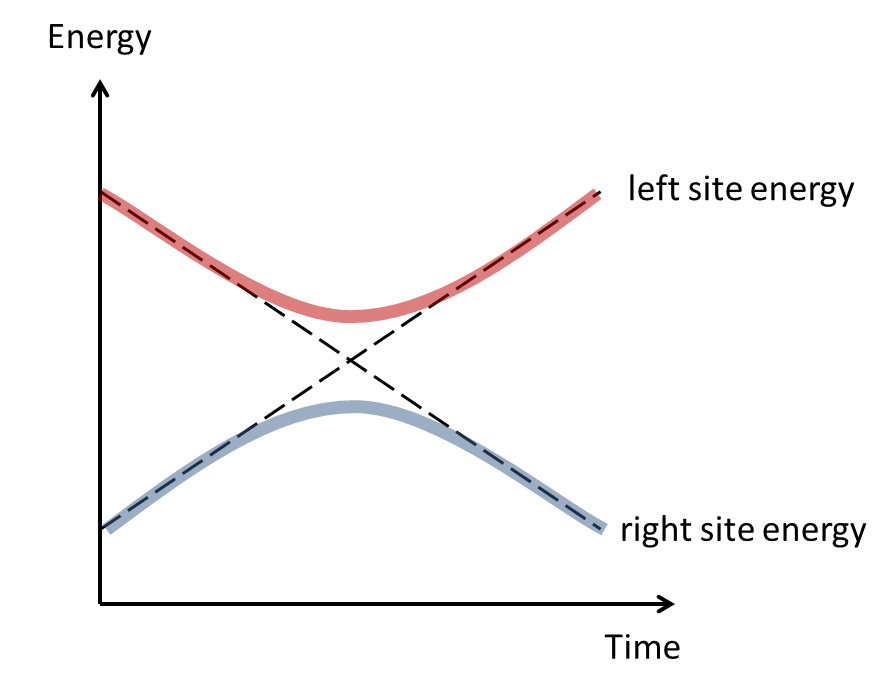
\includegraphics[width=0.75\textwidth]{images/avoided-crossing.png}
	\caption{Avoided crossing following Landau-Zener approximations.}
	\label{fig:LZ}
\end{figure}

In this simple system, two things can happen as we sweep $\Delta E$ (in time).  On the one hand, if we sweep very slowly (adiabatic), then eigenstates have time to ``adapt'' and remain at their relative energy levels, i.e., the lower-energy eigenstate will change its wavefunction so that its energy remains the lower energy, and vice versa. If we sweep very quickly (non-adiabatic), on the other hand, then the eigenstate may remain the same, with some probability of transitioning to other eigenstate(s). \\


What we mean by ``slowly'' and ``quickly'' will be captured in the adiabatic conditions in the next section. But the main point here is that the transition probability mentioned above is called the Landau-Zener transition probability, named after two physicists who stated and solved the problem (analytically). As we will see below, this probability is an exponential decay which depends on the sweeping rate (how slowly/quickly $\Delta E$ changes) and how strong the two states are coupled. 


\subsection*{Results for Linear LZ Sweep}

We will write the Hamiltonian with (possible) time dependence:
\begin{equation*}
\widehat{H} = \begin{bmatrix}
E_1(t) & E_{12}(t) \\ E_{12}(t)^* & E_{2}(t).
\end{bmatrix}
\end{equation*}



Landau and Zener's analytical solution arrived after making the following approximations and simplifications: 
\begin{itemize}
	\item $E_{12}$ is very small compared to $\Delta E$. We can treat it as constant.
	\item $\Delta E$ varies linearly in time 
\end{itemize}

From these simplifications we have, for all time, 
\begin{equation*}
\f{d}{dt}(E_1(t) - E_2(t)) = \al t \quad \text{ and } \quad \f{d}{dt}{E_{12}(t)} = 0.
\end{equation*}

To state the transition probability due to Landau and Zener, we must define it first. To this end, we first define the ``non-adiabatic'' basis by 
\begin{equation*}
\ket{1} = \begin{pmatrix}
1 \\ 0
\end{pmatrix} \quad \text{ and }  \quad
\ket{2} = \begin{pmatrix}
0 \\ 1
\end{pmatrix}
\end{equation*}

Next, let $\ket{\Psi(t)}$ solve the SE, then a natural ansatz for $\ket{\Psi(t)}$ is 
\begin{equation*}
\ket{\Psi(t)} = A(t) \exp \lp -\f{i}{\hbar}\int_0^{t} E_1(t')\,dt' \rp \ket{1} + B(t) \exp \lp -\f{i}{\hbar}\int_0^{t} E_2(t')\,dt' \rp \ket{2}.
\end{equation*}
We assume that at time $t=-\infty$, the system is in state $\ket{2}$, so that
\begin{equation*}
A(-\infty) = 0 \quad \text{ and } \quad B(-\infty) = 1.
\end{equation*}
We wish to find the probability $P$ that the system makes a transition from state $\ket{2}$ to $\ket{1}$, which is given by 
\begin{equation*}
P = \abs{B(\infty)}^2 = 1- \abs{A(\infty)}^2.
\end{equation*}
In his paper \cite{zener1932non}, Zener showed that 
\begin{equation*}
\boxed{P = e^{-2\pi \gamma}, \text{ where } \gamma = \f{\abs{E_{12}}^2}{\hbar \abs{\al}}} 
\end{equation*}
The derivation is quite nice. Zener casts the differential equation for $B(t)$ into the form of the \textbf{Weber's equation} and extracted the asymptotic behavior for $B(t)$ from there. 


\subsubsection*{Numerical verification}



Since the (analytical) derivation of the Landau-Zener transition probability is rather involved, we will only work with a numerical verification. This verification is inspired by Problem set 7 of MIT's 8.06: Quantum Physics III - Spring 2018. \\


We start by getting a set of ODEs for $A(t)$ and $B(t)$ from the SE:
\begin{align*}
i\hbar  \f{d}{dt}A(t) &= E_{12} B(t)  \exp\lp -\f{i}{\hbar} \int_0^t E_2(t') - E_1(t') \,dt'\rp\\
i\hbar  \f{d}{dt}B(t) &= E_{12}^* A(t)  \exp\lp +\f{i}{\hbar} \int_0^t E_2(t') - E_1(t') \,dt'\rp
\end{align*}
Let $E_1(t) - E_2(t) = \Delta E(t)$, then 
\begin{align*}
i\hbar  \f{d}{dt}A(t) &= E_{12} B(t)  \exp\lp +\f{i}{\hbar} \int_0^t \Delta E(t') \,dt'\rp\\
i\hbar  \f{d}{dt}B(t) &= E_{12}^* A(t)  \exp\lp -\f{i}{\hbar} \int_0^t \Delta E(t') \,dt'\rp
\end{align*}
This is a set of linear, first-order, coupled DEs. From here, we can get a second-order DE for $B$. To get a nice, unit-free equation, we let
\begin{equation*}
\tau = \f{\al}{\abs{E_{12}}} t \quad \text{ and } \quad \gamma = \f{\abs{E_{12}}^2}{\hbar \al}.
\end{equation*}
We then get
\begin{equation*}
\f{d^2 B}{d\tau^2} + i\gamma \tau \f{dB}{d\tau} + \gamma^2 B = 0.
\end{equation*}

We will solve this for $\gamma = 0.1$ and $\tau \in [-60, 60]$. MATLAB code for this: 
\begin{lstlisting}
% Huan Q. Bui
% 2nd order ODE solver for Landau-Zener problem

clear all
close all
global gamma

tspan = [-60 60];
B0 = 1;
C0 = 0;
gamma = 0.1;

[t,y] = ode45(@LZ_ODE,tspan,[B0; C0]);
% y(1) = B
% y(2) = C = \dot{B}

plot(t,abs(y(:,1)).^2,'LineWidth', 2)
title('|B(t)|^2 with \gamma = 0.1 using ODE45');
xlabel('Time t');
ylabel('|B(t)|^2');
grid on

% plot LZ prediction
yline(exp(-2*pi*gamma), 'LineWidth',2);

% legend
legend('|B(t)|^2', 'Exp(-2\pi\gamma)');

function dydt = LZ_ODE(t,y)
global gamma
dydt = [y(2); -1i*gamma.*t.*y(2) - gamma^2.*y(1)];
end

\end{lstlisting}



Plotting $\abs{B(\tau)}$ against $\tau$ and plotting the predicted $\exp(-2\pi \gamma) = \lim_{\tau\to\infty}\abs{B(\tau)}^2$, we find good agreement:
\begin{figure}[!htb]
	\centering
	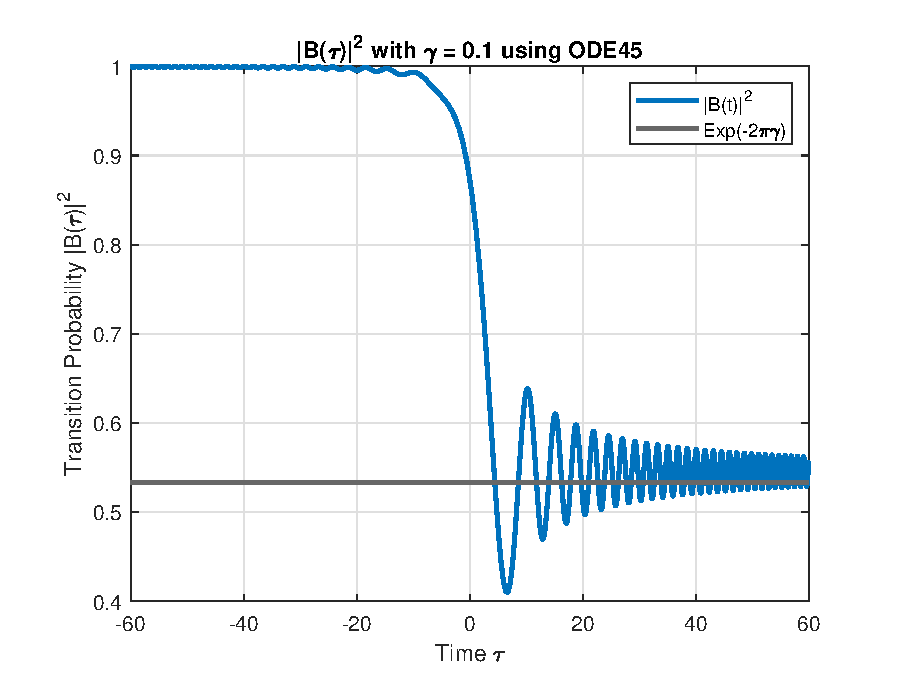
\includegraphics[width=0.75\textwidth]{images/LZ}
\end{figure}


We next test how well things agree by solving the ODE in $B(t)$ for a range of $\gamma$'s. We expect that as the time span of the solver is increased, $\abs{B(t_{\text{final}})}^2$ approach $\exp(-2\pi \gamma)$ better and better. See Figure \ref{fig:tau_Infty}.

\begin{figure}[!htb]
	\begin{minipage}{0.49\textwidth}
		\centering
		\includegraphics[width=\textwidth]{images/t050.eps}
		\caption{$\tau\in [-50,50]$}
		\includegraphics[width=\textwidth]{images/t100.eps}
		\caption{$\tau\in [-100,100]$}
	\end{minipage}
	\begin{minipage}{0.49\textwidth}
		\centering
		\includegraphics[width=\textwidth]{images/t200.eps}
		\caption{$\tau\in [-200,400]$}
		\includegraphics[width=\textwidth]{images/t400.eps}
		\caption{$\tau\in [-400,400]$}
	\end{minipage}
	\caption{$\abs{B(\tau)}^2$ approaches $\exp(-2\pi\gamma)$ as the $\tau$ goes to $\infty$. Here, $\gamma \in [0,1.5]$}
	\label{fig:tau_Infty}
\end{figure}


MATLAB code:
\begin{lstlisting}
% Huan Q. Bui
% Exponential decay in LZ transition probability

clear all
close all

% solve LZ ODE for these gammas
gamma = 0:0.05:1.5;
tspan = [-50 50];
B0 = 1;
C0 = 0;

B_list = [];

for g = gamma
[t,y] = ode45(@(t,y) LZ_ODE(t,y,g),tspan,[B0; C0]);
% y(1) = B
% y(2) = C = \dot{B}

% append the last B(t) = B(t=end) to B_list
B_list = [B_list abs(y(end,1))^2];
end


plot(gamma,B_list,'-o')
hold on
plot(gamma, exp(-2*pi*gamma), 'LineWidth', 1)
hold off
title('|B(t_{end})| and Exp(-2\pi\gamma) vs. \gamma')
xlabel('\gamma')
ylabel('Transition probability')
legend('|B(t_f)|', 'Exp(-2\pi\gamma)')
grid on

function dydt = LZ_ODE(t,y,g)
dydt = [y(2); -1i*g.*t.*y(2) - g^2.*y(1)];
end

\end{lstlisting}


%%%%%%%%%%%%%%%%%%%%%%%%%%%%%%%%%%%%%%%
\chapter*{M}



\section*{Magnetic Trap Designs}





\subsection*{Mathematica Notebook}
The Mathematica notebook which contains some calculations and sketches can be downloaded via this \href{https://raw.githubusercontent.com/huanium/huanium/master/MIT PhD/BUI_AtomicPhysics/mathematica/magnetic-traps.nb}{link}. Right-click and ``Save" to save the notebook to your computer. 


\subsection*{Zeeman Effect \& Earnshaw's Theorem}



\subsection*{Quadrupole trap (anti-Helmholtz)}

This section on the quadrupole trap and the next section on the TOP trap follow \cite{perez2013does}.

\subsubsection*{Calculation}


In this configuration, there are two coils of radius $a$ placed at distance $2b$ apart. Running through the coils are equal and opposite currents $I$ and $-I$, respectively. Here, we set $I = NI_0$ where $N$ is the number of coils and $I_0$ is the current going through each coil (or equivalently through all the coils).

\begin{figure}[!htb]
	\centering
	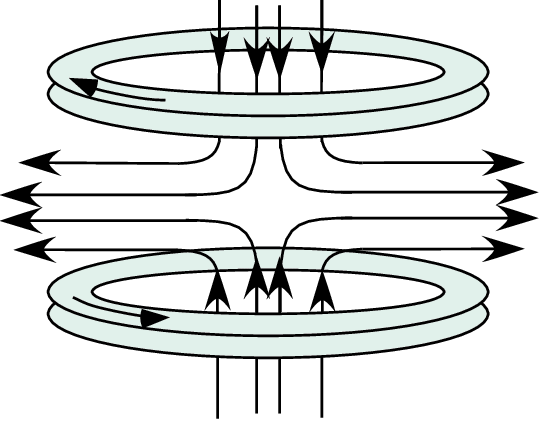
\includegraphics[width=0.6\textwidth]{images/antiHelmholtz.png}
	\caption{From \cite{maruyama2003optical}}
\end{figure}

To calculate the magnetic field for one coil, we can use Biot-Savart law because the current is constant. We will integrate along the closed loop $C$ defined by the coil. The relative position between the point $\mathbf{r}$ and the point $\vec{l}$ on the wire is given by $\vec{r}' = \vec{r} - \vec{l}$
\begin{equation*}
\vec{B}(\vec{r}) = \f{\mu_0 I}{4\pi} \int_C \f{d\vec{l} \times \vec{r}'}{ |{\vec{r}'}|^3} = \f{\mu_0 I}{4\pi} \int_C \f{d\vec{l} \times (\vec{r} - \vec{l})}{|{\vec{r} - \vec{l}}|^3}.  
\end{equation*}
We now make the approximation $|\vec{r}| \ll \vec{l}$ (i.e., we're interested in points far from the coil). With this we have the following expansion\footnote{a more accurate expansion will be presented in the section on the Ioffe-Pritchard trap. For our purposes in this section, it suffices to not include the term $-3|\vec{r}|^2/2|\vec{l}|^2$}
\begin{equation*}
\f{1}{|\vec{r} - \vec{l}|^3} \approx \f{1}{|\vec{l}|^3} + \f{3 \vec{r}\cdot \vec{l}}{|\vec{l}|^5} + \dots
\end{equation*}
Plugging this back in for $\vec{B}(\vec{r})$ we find 
\begin{equation*}
\vec{B}(\vec{r}) \approx \f{\mu_0 I}{4\pi}\int_C d\vec{l}\times \f{\vec{r} - \vec{l}}{|\vec{l}|^3} + \f{3\mu_0 I}{4\pi} \int_C d\vec{l} \times (\vec{r} - \vec{l}) \f{\vec{r}\cdot \vec{l}}{|\vec{l}|^5}.
\end{equation*}
Suppose that the center of the coil is at $+d$ from the $XY$ plane. Going into cylindrical coordinates, we have
\begin{equation*}
\vec{l} = a\cos\theta\hat{x} + a\sin\theta\hat{y} + d\hat{z}
\end{equation*}
from which we find 
\begin{equation*}
d\vec{l} = -a\sin\theta d\theta\hat{x} + a\cos\theta d\theta \hat{y}
\end{equation*}
So, we have
\begin{equation*}
d\vec{l} \times (\vec{r} - \vec{l}) = (-a\sin\theta, a\cos\theta,0)\times(x-a\cos\theta,y-a\sin\theta,z-d)
\end{equation*}
and 
\begin{equation*}
\vec{r}\cdot \vec{l} = xa\cos\theta + ya\sin\theta + za.
\end{equation*}
So, we have
\begin{equation*}
\f{\mu_0 I}{4\pi}\int_C d\vec{l}\times \f{\vec{r} - \vec{l}}{|\vec{l}|^3} = \f{\mu_0 I }{4\pi} \f{2a^2 \pi}{(d^2 + a^2)^{3/2}} \hat{z} = \f{\mu_0 I a^2}{2(d^2 + a^2)^{3/2}} \hat{z}.
\end{equation*}
and 
\begin{align*}
&\f{3\mu_0 I }{4\pi}\int_C d\vec{l}\times (\vec{r} - \vec{l}) \f{\vec{r}\cdot \vec{l}}{|\vec{l}|^5}\\ 
=\,\, &\f{3\mu_0 Ia^2}{4(d^2+a^2)^{5/2}} \left(- x(d-z)\hat{x}  - y (d-z)\hat{y} -  (x^2 + y^2 - 2dz)\hat{z}\right).
\end{align*}
Keeping only the linear terms and combining everything, we find the total field:
\begin{align*}
\vec{B}(\vec{r}) &= \f{\mu_0 I a^2}{2(d^2 + a^2)^{3/2}} \hat{z} + \f{3\mu_0 Ia^2}{4(d^2+a^2)^{5/2}} \left(- xd\hat{x}  -  y d\hat{y} - 2dz\hat{z}\right)\\
&= \f{\mu_0 I a^2}{2(d^2 + a^2)^{3/2}} \hat{z} + \f{3\mu_0 Ia^2 d}{2(d^2+a^2)^{5/2}} \left(- \f{x}{2}\hat{x}  -  \f{y}{2}\hat{y} - z\hat{z}\right).
\end{align*}






In the anti-Helmholtz configuration, we have two coils of radius $a$ placed a distance $2b$ apart from each other. When summing the two fields to get the total field, the first term cancels. So we get
\begin{equation*}
\vec{B}_\text{tot}(\vec{r}) = \vec{B}_{+b}(\vec{r}) + \vec{B}_{-b}(\vec{r}) = -\f{3\mu_0 I a^2 b}{2(a^2 + b^2)^{5/2}}\left( x,y,-2z \right) \equiv B_0 (x,y,-2z).
\end{equation*}
The field strength is given by 
\begin{equation*}
\abs{B(\vec{r})} = B_0 \sqrt{x^2 + y^2 + 4z^2}.
\end{equation*}

We notice that this trap is not harmonic. Further, there is a zero minimum of the magnetic field. When particles reach the zero minimum, the Zeeman shifts are reduced, leading to a loss of particles in the trap. The escape mechanism is called the Majorana spin-flip transition which we will discuss later. 


\subsubsection*{Trap parameters}

\subsubsection*{Simulation}


The quadrupole trap is the simplest magnetic trap configuration. The MATLAB code for this simulation is included below the figures. The code is perhaps not the most efficient way to do things, but this simulation is simple enough that we won't worry about such things for now. 


\begin{figure}[!htb]
	\centering
	\begin{minipage}{.33\textwidth}
		\centering
		\includegraphics[width=\linewidth]{sim-figs/quad-1.eps}
	\end{minipage}%
	\begin{minipage}{.33\textwidth}
		\centering
		\includegraphics[width=\linewidth]{sim-figs/quad-2.eps}
	\end{minipage}%
	\begin{minipage}{.33\textwidth}
		\centering
		\includegraphics[width=\linewidth]{sim-figs/quad-3.eps}
	\end{minipage}%
\end{figure}


\begin{lstlisting}
% Author: Huan Q. Bui
% Date: August 10, 2021

% SIMULATE Anti-Helmholtz magnetic field

clear

mu0 = 4*pi*10^(-7);
I = 10; % current in each coil, in Amperes
N = 16; % winding number
a = 0.2; % coil radius, in m
b = 0.15; % 1/2 distance between coils, in m
C = 3*mu0*I*a^2*b/(2*(a^2 + b^2)^(5/2)); % constant

x_bound = 1;
y_bound = 1;
z_bound = 1;
spacing = 0.2;

x = -x_bound:spacing:x_bound;
y = -y_bound:spacing:y_bound;
z = -z_bound:spacing:z_bound;

[X,Y,Z] = meshgrid(x,y,z);

% magnetic fields formula
% Bfield = @(x,y,z) [C.*x C.*y -2*C.*z]; 
% Bfield_XZ = @(x,z) [C.*x -2*C.*z];

h = figure(1)

% magnetic field in XZ plane
subplot(3,1,1)
quiver(X,Z,C.*X,-2*C.*Z);
xlabel('X (m)')
ylabel('Z (m)')
title('Field in XZ plane, Y=0')
xlim([-x_bound x_bound])
ylim([-z_bound z_bound])


subplot(3,1,2)
% magnetic field in YZ plane
quiver(Y,Z,C.*Y,-2*C.*Z);
xlabel('Y (m)')
ylabel('Z (m)')
title('Field in YZ plane, X=0')
xlim([-y_bound y_bound])
ylim([-z_bound z_bound])

subplot(3,1,3)
% magnetic field in XY plane
quiver(X,Y,C.*X,C.*Y);
xlabel('X (m)')
ylabel('Y (m)')
title('Field in XY plane, Z=0')
xlim([-x_bound x_bound])
ylim([-y_bound y_bound])


% Magnetic field strengths in 2D
g = figure(2)

subplot(3,1,1)
[X_XZ,Z_XZ] = meshgrid(x,z);
B_strength_XZ = sqrt((C.*X_XZ).^2  + (-2*C.*Z_XZ).^2);
surfc(X_XZ,Z_XZ,B_strength_XZ,'LineStyle' ,'none');
view(2)
xlabel('X (m)')
ylabel('Z (m)')
title('Field strength (T) in XZ, Y=0')

subplot(3,1,2)
[Y_YZ,Z_YZ] = meshgrid(y,z);
B_strength_YZ = sqrt((C.*Y_YZ).^2  + (-2*C.*Z_YZ).^2);
surfc(Y_YZ,Z_YZ,B_strength_YZ,'LineStyle' ,'none');
view(2)
xlabel('Y (m)')
ylabel('Z (m)')
title('Field strength (T) in YZ, X=0')

subplot(3,1,3)
[X_XY,Y_XY] = meshgrid(x,y);
B_strength_XY = sqrt((C.*X_XY).^2  + (-2*C.*Y_XY).^2);
surfc(X_XY,Y_XY,B_strength_XY,'LineStyle' ,'none');
view(2)
xlabel('X (m)')
ylabel('Y (m)')
title('Field strength (T) in XY, Z=0')

% magnetic field strengths in 1D
k = figure(3)
% X=0,Y=0
subplot(3,1,1)
plot(z,abs(-2*C.*z))
xlabel('Z (m)')
ylabel('B (T)')
title('Field strength in Z')
% Y=0,Z=0
subplot(3,1,2)
plot(x, abs(C.*x))
xlabel('X (m)')
ylabel('B (T)')
title('Field strength in X')
% X=0,Z=0
subplot(3,1,3)
plot(y, abs(C.*y))
xlabel('Y (m)')
ylabel('B (T)')
title('Field strength in Y')

\end{lstlisting}



\newpage

\subsection*{TOP trap}


\subsubsection*{Calculation}

As will be discussed later, the quadrupole or anti-Helmholtz trap suffers from the ``Majorna spin-flip problem'' which occurs due to the presence of a zero-magnetic field point in the trap. To overcome this issue, one can add a rotating magnetic field to the existing anti-Helmholtz field so that the time-averaged magnetic field no longer has a zero at the center. This trick gives us the TOP (time orbiting potential) trap. The total field is given by 
\begin{equation*}
\vec{B}(\vec{r},t) = \vec{B}_\text{quad}(\vec{r}) + \vec{B}_b(\vec{r}) = B_0 (x,y,-2z) + B_b(\cos\Omega t, \sin\Omega t,0),
\end{equation*} 
where $\Omega$ is the angular frequency of the rotating field. \\


The field strength is given by 
\begin{equation*}
B(\vec{r},t) = \sqrt{(B_0 x + B_b\cos\Omega t)^2 + (B_0 y + B_b\sin\Omega t)^2 + 4 B_0^2 z^2 }
\end{equation*}

\begin{figure}[!htb]
	\centering
	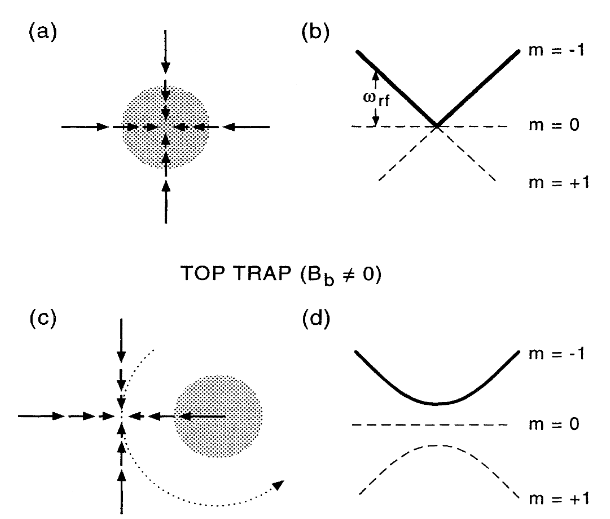
\includegraphics[width=0.6\textwidth]{images/TOP_trap.png}
	\caption{From \cite{PhysRevLett.74.3352}. By rotating the trap in the $XY$ plane fast enough, the atoms see a time-averaged trap that is not only quadratic (harmonic) but also has no zero minimum when $B_b \neq 0$. We note, however, that the harmonic potential is anisotropic: there is stronger confinement in the $z$-direction.}
	\label{fig:cornell}
\end{figure}

For this trap to work $\Omega$ can't be too small or too large. $\Omega$ must be larger than the oscillation frequency of the trapped particles (which is on the order of $100$ Hz) so that the particles feel an effective time-averaged magnetic field. $\Omega$ should also be smaller than the frequency associated with the transition between two adjacent internal quantum states (which is on the order of $1$ MHz) in order to prevent particle losses due to Majorana spin-flips. \\


We are interested in dynamics near the center of the trap, so we can make the approximation $r = \sqrt{x^2 + y^2 + z^2} \ll a$, under which 
\begin{equation*}
B(\vec{r},t)\approx B_b + \f{B_0^2}{2B_b^2} (x^2 + y^2 + 4z^2) + \f{B_0}{B_b}(x\cos\Omega t+ y\sin\Omega t) - \f{B_0^2}{2B_b^2}(x\cos\Omega t + y\sin\Omega t)^2.
\end{equation*}
The time-averaged magnetic field strength is thus, by inspection,
\begin{align*}
\langle B \rangle 
&= B_b  + \f{B_0^2}{2B_b^2} (x^2 + y^2 + 4z^2) - \f{B_0^2}{2B_b^2}\lp \f{x^2}{2} + \f{y^2}{2}\rp\\ &= B_b + \f{B_0^2}{4B_b}(x^2 + y^2 + 8z^2).
\end{align*}


\subsubsection*{Trap parameters}
Here we want to calculate the trapping frequencies for the trap. Recall that the energy of a magnetic dipole moment $\mu$ acted by an external magnetic field $B$ is given by 
\begin{equation*}
E = -\mu |B|,
\end{equation*}
where $\mu \sim g_F m_F \mu_B$ (more explicit expressions for $\vec{\mu}$ which involves the spin $s$ and orbital $l$ $g$-factors can be found elsewhere).\\ 

Assuming that the energy goes like the energy for harmonic oscillation. Consider the $x$-direction with $y=z=0$ and ignoring the offset, we find
\begin{equation*}
E \sim \f{1}{2}m_\text{atom} \omega_x^2 x^2 = -\mu B = -\mu \f{B_0^2}{4B_b}x^2.
\end{equation*}
This gives
\begin{equation*}
\omega_x = \sqrt{\f{-\mu B_0^2}{2B_b m_\text{atom}}}.
\end{equation*}
By symmetry,
\begin{equation*}
\omega_y = \sqrt{\f{-\mu B_0^2}{2B_b m_\text{atom}}}
\end{equation*}
Similarly, for $z$:
\begin{equation*}
\omega_z = \sqrt{\f{-4\mu B_0^2}{B_b m_\text{atom}}}.
\end{equation*}
The aspect ratio is given by 
\begin{equation*}
\Lambda = \f{\omega_\rho}{\omega_z} = \f{\omega_x}{\omega_z} = {\f{1}{2\sqrt{2}}}.
\end{equation*}


We see that this trap works for $\mu < 0$, implying that the states are low-field seeking (so that $E = -\mu |B|$ is minimized). 

\subsubsection*{Simulation}


The magnetic field at any given time (or instantaneous magnetic field) is simply the quadrupole magnetic field plus some shift in the $XY$ plane (as shown in Figure \ref{fig:cornell}), so we don't have to reproduce it here. The simulation only shows the time-averaged field. Once again, the (probably inefficient) MATLAB code is attached below the figures.




\begin{figure}[!htb]
	\centering
	\begin{minipage}{.49\textwidth}
		\centering
		\includegraphics[width=\linewidth]{sim-figs/TOP-1.eps}
	\end{minipage}%
	\begin{minipage}{.49\textwidth}
		\centering
		\includegraphics[width=\linewidth]{sim-figs/TOP-2.eps}
	\end{minipage}%
\end{figure}



\begin{lstlisting}
% Author: Huan Q. Bui
% Date: August 10, 2021

% SIMULATE TOP magnetic trap

clear

mu0 = 4*pi*10^(-7);
I = 1; % current in each coil, in Amperes
N = 16; % winding number
a = 0.2; % coil radius, in m
b = 0.15; % 1/2 distance between coils, in m
C = 3*mu0*I*a^2*b/(2*(a^2 + b^2)^(5/2)); % constant
B = 2*C;

x_bound = 10;
y_bound = 10;
z_bound = 10;
spacing = 0.1;

x = -x_bound:spacing:x_bound;
y = -y_bound:spacing:y_bound;
z = -z_bound:spacing:z_bound;

[X,Y,Z] = meshgrid(x,y,z);

% field strength formula:
% Bstrength = B + (C^2/(4*B))*(x^2 + y^2 + 8z^2);


% Magnetic field strengths in 2D
g = figure(1)

subplot(3,1,1)
[X_XZ,Z_XZ] = meshgrid(x,z);
B_strength_XZ = B + (C^2/(4*B))*(X_XZ.^2 + 8.*Z_XZ.^2);
surfc(X_XZ,Z_XZ,B_strength_XZ,'LineStyle' ,'none');
view(2)
xlabel('X (m)')
ylabel('Z (m)')
title('Field strength (T) in XZ, Y=0')

subplot(3,1,2)
[Y_YZ,Z_YZ] = meshgrid(y,z);
B_strength_YZ = B + (C^2/(4*B))*(Y_YZ.^2 + 8.*Z_YZ.^2);
surfc(Y_YZ,Z_YZ,B_strength_YZ,'LineStyle' ,'none');
view(2)
xlabel('Y (m)')
ylabel('Z (m)')
title('Field strength (T) in YZ, X=0')

subplot(3,1,3)
[X_XY,Y_XY] = meshgrid(x,y);
B_strength_XY = B + (C^2/(4*B))*(X_XY.^2 + Y_XY.^2);
surfc(X_XY,Y_XY,B_strength_XY,'LineStyle' ,'none');
view(2)
xlabel('X (m)')
ylabel('Y (m)')
title('Field strength (T) in XY, Z=0')

% magnetic field strengths in 1D
k = figure(2)
% X=0,Y=0
subplot(3,1,1)
plot(z,B + (C^2/(4*B)).*(8*z.^2))
xlabel('Z (m)')
ylabel('B (T)')
title('Field strength in Z')
% Y=0,Z=0
subplot(3,1,2)
plot(x, B + (C^2/(4*B)).*(x.^2))
xlabel('X (m)')
ylabel('B (T)')
title('Field strength in X')
% X=0,Z=0
subplot(3,1,3)
plot(y, B + (C^2/(4*B)).*(y.^2))
xlabel('Y (m)')
ylabel('B (T)')
title('Field strength in Y')

\end{lstlisting}



\newpage


\subsection*{Ioffe-Pritchard traps}

This section will essentially follow \cite{allcoil} except for the calculation of the magnetic field produced by a coil. Instead of doing an expansion using Legendre polynomials and using power series expansion of the magnetic potential $\Psi$ (where $\vec{B} = \nabla \Psi$), here we simply do a series expansion for integrand of the Biot-Savart law integral and pick out terms of the same orders.  



\begin{figure}[!htb]
	\centering
	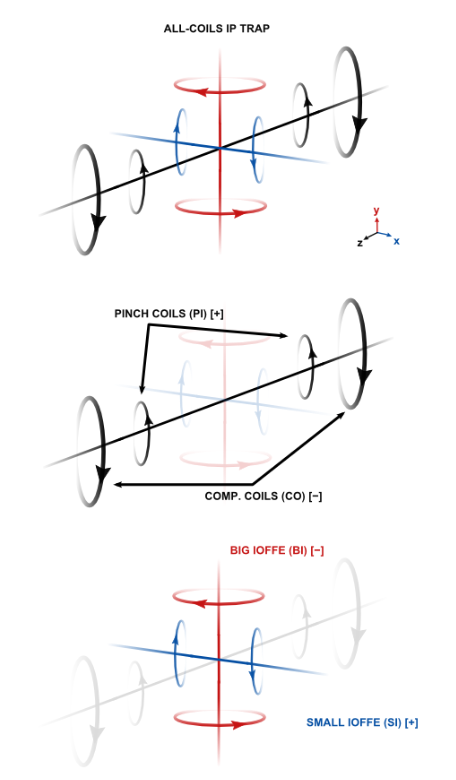
\includegraphics[width=0.75\textwidth]{images/all-coils.png}
	\caption{From \cite{allcoil}}
\end{figure}

\subsubsection*{Calculation}


There are many variants of the IP trap, the simplest being one with two coils in the anti-Helmholtz configuration and four wires in the $z$-direction. The four wires are suited at the corners of a square, with the currents flowing along adjacent wires being of opposite sign. A generalization of the IP trap is often called the ``all coils Ioffe-Pritchard trap.'' The all-coil trap consists of the following set of coils:
\begin{itemize}
	\item Big Ioffe Coils (BI), anti-Helmholtz, along $z$
	\item Small Ioffe Coils (SI), anti-Helmholtz, along $x$
	\item Pinch coils (PI), Helmholtz, along $y$
	\item Compensation coils (CO), Helmholtz, along $y$, opposite current to SI.
\end{itemize}

Let us revisit the calculation we've done for Helmholtz and anti-Helmholtz coils, but now we will expand to higher orders (still assuming that $\vec{r}$ is near the origin). In particular, we will use
\begin{equation*}
\f{1}{|\vec{r} - \vec{l}|^3} \approx \f{1}{|\vec{l}|^3} 
\lb 1 -\f{3}{2}\epsilon
+ \f{15}{8}\epsilon^2 
- \f{35}{16}\epsilon^3 \rb
\end{equation*}
where
\begin{equation*}
\epsilon = \f{|\vec{r}|^2}{|\vec{l}|^2} - \f{2\vec{r}\cdot\vec{l}}{|\vec{l}|^2}.
\end{equation*}
The expansion can be obtained by following 
Eq. 3.88 of \cite{griffiths2005introduction}. We notice the difference between this expansion and the expansion that appeared in the section on the anti-Helmholtz configuration. Here, we include the term $\abs{\vec{r}}/\abs{\vec{l}}$ in $\epsilon$, so that the expansion is more accurate and match the result due to expansion in Legendre polynomials presented in \cite{allcoil}.\\


For a single coil with current $I$ placed a vertical distance $+d$ from the origin, we find the factor $|\vec{l}| = \sqrt{a^2 + d^2}$ to be constant. The field, order-by-order to third order, is thus  
\begin{equation*}
B^{(0)}(\vec{r}) = \f{\mu_0 I}{4\pi |\vec{l}|^3}\int_C d\vec{l}\times (\vec{r} - \vec{l}) = \f{1}{2}\f{\mu_0 I a^2}{(a^2 + d^2)^{3/2}} \hat{z}
\end{equation*}
\begin{align*}
B^{(1)}(\vec{r}) 
&= \f{3\mu_0 I}{4\pi |\vec{l}|^5}\int_C d\vec{l}\times (\vec{r} - \vec{l}) \lp \f{|\vec{r}|^2}{|\vec{l}|^2} - \f{2\vec{r}\cdot\vec{l}}{|\vec{l}|^2} \rp
\end{align*}
\begin{align*}
B^{(2)}(\vec{r}) 
&= \f{15\mu_0 I}{8\pi |\vec{l}|^7}\int_C d\vec{l}\times (\vec{r} - \vec{l}) \lp \f{|\vec{r}|^2}{|\vec{l}|^2} - \f{2\vec{r}\cdot\vec{l}}{|\vec{l}|^2} \rp^2
\end{align*}
\begin{align*}
B^{(3)}(\vec{r}) &= \f{35\mu_0 I}{8\pi |\vec{l}|^9}\int_C d\vec{l}\times (\vec{r} - \vec{l}) \lp \f{|\vec{r}|^2}{|\vec{l}|^2} - \f{2\vec{r}\cdot\vec{l}}{|\vec{l}|^2} \rp^3
\end{align*}
All these integrals can be done in Mathematica. The total field is found by summing the integrals. Collecting the terms order-by-order to third order (in $z$ and $\rho$) and defining $\rho^2 = x^2 + y^2$ we find that
\begin{align*}
\f{B_z(z,\rho)}{\mu_0 I} \approx &\,\,\f{1}{2}\f{a^2}{(a^2+d^2)^{3/2}} + \f{3da^2}{2(a^2+d^2)^{5/2}}z 
\\
&+ \f{3a^2(4d^2 - a^2)}{4(a^2+d^2)^{7/2}} \lp z^2 - \f{\rho^2}{2} \rp
+\f{5 a^2 d (4d^2 - 3 a^2)}{4 (a^2 + d^2)^{9/2}}\lp z^3 - \f{3 z\rho^2}{2}\rp\\
\equiv&\,\, \f{1}{2}\mathbb{F} + \mathbb{G}z + \f{1}{4}\mathbb{H}\lp z^2 - \f{\rho^2}{2} \rp + \f{1}{2} \mathbb{I}\lp z^3 - \f{3 z\rho^2}{2}\rp
\end{align*}
where 
\begin{equation*}
\mathbb{F} = \f{a^2}{(a^2+d^2)^{3/2}}, \quad 
\mathbb{G} = \f{3da^2}{2(a^2+d^2)^{5/2}}, \quad 
\mathbb{H} = \f{3a^2(4d^2-a^2)}{(a^2+d^2)^{7/2}},\quad
\mathbb{I} = \f{5 a^2 d (4 d^2-3a^2)}{2(a^2 + d^2)^{9/2}} 
\end{equation*}
are purely geometric factors. Following similar steps, we can find the field in the radial direction:
\begin{align*}
\f{B_\rho}{\mu_0 I} 
&\approx \f{\sqrt{B_x^2 + B_y^2}}{\mu_0 I} \\
&= \mathbb{G}\lp -\f{\rho}{2} \rp + \f{1}{4}\mathbb{H}(-\rho z) + \f{1}{2}\mathbb{I}\lp \f{3\rho^3}{8} - \f{3\rho z^2}{2} \rp.
\end{align*}

In these equations, we can interpret $\mathbb{F}$ as the component of the bias field, $\mathbb{G}$ of the field's gradient, and $\mathbb{H}$ of field curvature.  By symmetry, there is no field in the $\phi$ direction. 


\paragraph*{Field by Helmholtz pair}
To transform from one Helmholtz coil to the other in the Helmholtz configuration, we do the following:
\begin{equation*}
I \to I, \quad d \to -d.
\end{equation*}
With this, we can easily compute the total field.  
\begin{align*}
&B_z(z,\rho) \approx \mu_0 I \lb \mathbb{F} + \f{1}{2}\mathbb{H} \lp z^2 - \f{\rho^2}{2} \rp  \rb\\
&B_\rho(z,\rho) \approx \mu_0 I \lb \f{1}{2}\mathbb{H}(-\rho z) \rb.
\end{align*}
The other terms vanish since they are odd functions in $d$. We notice that this file only has a bias and curvature components. By letting $a=2d$ we can make  $\mathbb{H}$ vanish, producing a nearly constant field in $\hat{z}$ and almost no field in $\rho$. On the other hand, setting $a = d\sqrt{4/3}$ produces maximal $\mathbb{H}$ (maximal curvature). 



\paragraph*{Field by anti-Helmholtz pair}

To transform from one Helmholtz coil to the other in the anti-Helmholtz configuration, we do the following:
\begin{equation*}
I \to -I, \quad d \to -d.
\end{equation*}
With this, we can easily compute the total field:
\begin{align*}
&B_z(z,\rho) \approx  \mu_0 I \lb 2\mathbb{G}z + \mathbb{I}\lp z^3 - \f{3z\rho^2}{2} \rp \rb\\
&B_\rho(z,\rho) \approx \mu_0 I \lb -\mathbb{G}\rho + \mathbb{I}\lp \f{3\rho^3}{8} - \f{3\rho z^2}{2} \rp \rb
\end{align*}
where now the terms that are even in $d$ vanish. We notice that $\mathbb{I} = 0$ when $a = d\sqrt{4/3}$. Thus, configuring the field this way cancels out higher order terms. On the other hand, $\mathbb{G}$ is maximal at $a = 2d$. 




\paragraph*{Ioffe-Pritchard trap}
With the fields calculated, we now just plug everything in and find the total field in the Ioffe-Pritchard configuration. \\

We start with the big Ioffe coils (BI) in the anti-Helmholtz configuration. We will impose the condition $a_{BI} = d_{BI}\sqrt{4/3}$ so that $\mathbb{I}_{BI} = 0$. In Cartesian coordinates, this field is 
\begin{equation*}
\vec{B}_{BI}(x,y,z) = \mu_0 I_{BI} \mathbb{G}_{BI}(-x,-y,2z ).
\end{equation*}
In practice, $BI$ coils have $y$ as their symmetry axis, with current running in the opposite direction. The correct expression for the field is thus 
\begin{equation*}
\vec{B}_{BI}(x,y,z) = \mu_0 I_{BI} \mathbb{G}_{BI}(x,-2y,z).
\end{equation*}

For the small Ioffe coils, $x$ is the symmetry axis. We also impose the condition $a_{SI} = d_{SI}\sqrt{4/3}$ so that $\mathbb{I}_{SI} = 0$. Since they're also in the anti-Helmholtz configuration we have
\begin{equation*}
\vec{B}_{SI}(x,y,z) = \mu_0 I_{SI} \mathbb{G}_{SI} (2x,-y,-z).
\end{equation*}

For the pinch coils (PI) which are in the Helmholtz configuration, we find 
\begin{equation*}
\vec{B}_{PI}(x,y,z) = \mu_0 I_{PI} \lp -\f{1}{2}\mathbb{H}_{PI}xz,  -\f{1}{2}\mathbb{H}_{PI}yz, \mathbb{F}_{PI} + \f{1}{2}\mathbb{H}_{PI} \lp z^2 - \rho^2/2 \rp \rp.
\end{equation*}

Finally, we have the compensation coils (CO), which are in the Helmholtz configuration, but the current is in the opposite direction to PI's. The field is 
\begin{equation*}
\vec{B}_{CO}(x,y,z) = \mu_0 I_{CO} \lp \f{1}{2}\mathbb{H}_{CO}xz,  \f{1}{2}\mathbb{H}_{CO}yz, -\mathbb{F}_{CO} - \f{1}{2}\mathbb{H}_{CO} \lp z^2 - \rho^2/2 \rp \rp.
\end{equation*}

Adding everything up we find the full field:
\begin{align*}
\vec{B}(x,y,z) = 
&\begin{pmatrix}
0\\
0\\ 
\mu_0 I_{PI} \mathbb{F}_{PI} - \mu_0 I_{CO} \mathbb{F}_{CO} 
\end{pmatrix}
+ 
\begin{pmatrix}
(\mu_0 I_{BI}\mathbb{G}_{BI}  +2 \mu_0 I_{SI} \mathbb{G}_{SI}  )x\\
-(2\mu_0 I_{BI}\mathbb{G}_{BI} +\mu_0 I_{SI} \mathbb{G}_{SI})y\\
(\mu_0 I_{BI} \mathbb{G}_{BI} - \mu_0 I_{SI} \mathbb{G}_{SI})z
\end{pmatrix}\\
&+ \f{1}{2} \lp \mu_0 I_{PI}\mathbb{H}_{PI} -\mu_0 I_{CO}\mathbb{H}_{CO}  \rp \begin{pmatrix}
-xz\\-yz\\z^2 - \rho^2/2
\end{pmatrix}.
\end{align*}
We now add another constraint:
\begin{equation*}
\mu_0 I_{BI} \mathbb{G}_{BI} = \mu_0 I_{SI} \mathbb{G}_{SI}
\end{equation*}
so that the full field simplifies to:
\begin{align*}
\vec{B}(x,y,z) = 
\delta \begin{pmatrix}
0\\
0\\ 
1
\end{pmatrix}
+ 
\al \begin{pmatrix}
x\\
-y\\
0
\end{pmatrix}
+ \f{1}{2}\beta \begin{pmatrix}
-xz\\-yz\\z^2 - \rho^2/2
\end{pmatrix}
\end{align*}
where
\begin{align*}
&\al = 3\mu_0 I_{BI}\mathbb{G}_{BI} = 3\mu_0 I_{SI}\mathbb{G}_{SI}\\
&\beta = \mu_0 I_{PI}\mathbb{H}_{PI} -\mu_0 I_{CO}\mathbb{H}_{CO} \\
&\delta = \mu_0 I_{PI} \mathbb{F}_{PI} - \mu_0 I_{CO} \mathbb{F}_{CO} .
\end{align*}



\subsubsection*{Trap parameters}

Just as before, we want to calculate the trapping frequencies. Following a similar approach, we find the trapping frequency in the $z$-direction by setting $x=y=0$ and calculate $|\vec{B}|$ then extract $\omega_z$:
\begin{equation*}
\f{1}{2}m_\text{atom} \omega_z^2 z^2 = g_F m_F \mu_B\f{1}{2}\beta z^2
\end{equation*}
from which we find 
\begin{equation*}
\omega_z = \sqrt{\f{ g_F m_F \mu_B \beta}{m_\text{atom}}} = \sqrt{\f{g_F m_F \mu_B\mu_0 }{m_\text{atom}}\lp I_{PI}\mathbb{H}_{PI} - I_{CO}\mathbb{H}_{CO} \rp }.
\end{equation*}
Similarly, setting $z=0$ we find the field strength to be 
\begin{align*}
|\vec{B}| &= \sqrt{\al^2 \rho^2 + \delta^2 - \f{1}{2}\delta \beta \rho^2 + \cancel{\f{1}{16}\be^2 \rho^4}}\\
&\approx \sqrt{\delta^2 + \lp  \al^2 - \f{1}{2}\delta \beta\rp\rho^2} \\
&= \delta \sqrt{1 + \lp \f{\al^2}{\delta^2} - \f{\beta}{2\delta} \rp\rho^2 }\\
&\approx \delta \lb 1 + \f{1}{2}\lp \f{\al^2}{\delta^2} - \f{\be}{2\delta} \rp \rho^2 \rb\\
&= \delta + \f{1}{2}\lp \f{\al^2}{\delta} - \f{\beta}{2} \rp \rho^2
\end{align*}
As before, we only care about the curvature part:
\begin{equation*}
\f{1}{2}m_\text{atom} \omega_\rho^2 \rho^2 = g_F m_F \mu_B \f{1}{2}\lp \f{\al^2}{\delta} - \f{\beta}{2} \rp\rho^2
\end{equation*}
which gives
\begin{align*}
\omega_\rho &= \sqrt{\f{g_F m_F \mu_B}{m_\text{atom}} \lp \f{\al^2}{\delta} - \f{\be}{2} \rp  } \\
&= \sqrt{\f{g_F m_F \mu_B \mu_0}{m_\text{atom}} \lp \f{9I_{BI}\mathbb{G}_{BI}^2}{ I_{PI} \mathbb{F}_{PI} -  I_{CO} \mathbb{F}_{CO} }  - \f{ I_{PI}\mathbb{H}_{PI} - I_{CO}\mathbb{H}_{CO}}{2} \rp }.
\end{align*}



We can put on more constraints to further simplify things. In particular, we can let $a_{CO} = 2d_{CO}$ so that $\mathbb{H}_{CO} = 0$, meaning that the compensation coils only contribute to the bias field. With this constraint, we have
\begin{equation*}
\omega_z = \sqrt{\f{g_F m_F \mu_B\mu_0 }{m_\text{atom}} I_{PI}\mathbb{H}_{PI}  }
\end{equation*}
\begin{equation*}
\omega_\rho = \sqrt{\f{g_F m_F \mu_B \mu_0}{m_\text{atom}} \lp \f{9I_{BI}\mathbb{G}_{BI}^2}{ I_{PI} \mathbb{F}_{PI} -  I_{CO} \mathbb{F}_{CO} }  - \f{ I_{PI}\mathbb{H}_{PI} }{2} \rp }.
\end{equation*}


As before, the aspect ratio can be calculated via
\begin{equation*}
\Lambda = \f{\omega_\rho}{\omega_z}.
\end{equation*}



\subsubsection*{Simulation}
As opposed to the MATLAB code provided in \cite{allcoil}, the simulation below uses the expression for $\vec{B}$ which approximates to third order the total magnetic field near the center of the trap. The reader may refer to \cite{allcoil} for the exact simulation for the full field, evaluates the fields due to the coils exactly using numerical integration of elliptic integrals. The reader are also welcomed to compare the results generated using the approximate simulation presented here and those from the full simulation of \cite{allcoil}.\\


First, we reproduce the first simulation of \cite{allcoil} where $N = 16, \delta = 5$G, $I_{SI} 50$A, and $I_{PI}=12$A. All calculated parameters are listed below the figure. They agree well with the exact simulation provided by \cite{allcoil}. Next, without changing any parameters, we reproduce the fields in the $XY,YZ,ZX$ planes.


\begin{figure}[!htb]
	\centering
	
	\begin{minipage}{.49\textwidth}
		\centering
		\includegraphics[width=\linewidth]{sim-figs/IP-1.eps}
	\end{minipage}%
	\begin{minipage}{.49\textwidth}
		\centering
		\includegraphics[width=\linewidth]{sim-figs/IP-2.eps}
	\end{minipage}%
	\caption{Simulation with $N = 16, \delta = 5$G, $I_{SI} = 50$A, and $I_{PI}=12$A. We see the ``pencil'' like aspect ratio in the profile of $|B|$ in the $XZ$ and $YZ$ planes, signifying axial confinement. Calculated parameters shown below.}
\end{figure}


\begin{lstlisting}
-----------------------
Omega_Z: 20.4911 rad/s
Omega_Rho: 203.7857 rad/s
Aspect Ratio: 9.9451
-----------------------
delta: 5 G
alpha: 80.5921 G/cm
beta: 13.068 G/cm^2
-----------------------
J_BI: 112.6733 A
J_SI: 50 A
J_CO: 12.7507 A
J_PI: 12 A
-----------------------
a_BI: 5.2 cm
a_SI: 3.464 cm
a_CO: 5 cm
a_PI: 2.5 cm
-----------------------
d_BI: 4.5033 cm
d_SI: 2.9999 cm
d_CO: 2.5 cm
d_PI: 2.1651 cm
-----------------------
\end{lstlisting}

By modifying the parameters and removing some of the constraints, one can generate more ``interesting'' profiles shown in \cite{allcoil}. However we won't worry about that here. 



\newpage





\subsection*{The Majorana spin-flip problem}

















\section*{Magic wavelength}



From Wikipedia: Magic wavelength is the wavelength of an optical lattice at which the polarizabilities of two atomic clock states have the same values such that the AC Stark shift caused by the laser \textit{intensity} fluctuation has no effect on the transition frequency between the two clock states.\\


This is really all we need to know about the magic wavelength. Basically, the electric field due to the light for the optical lattice induces an electric dipole moment in the atoms to exert forces on them. This force depends on the location of the atom as well as the intensity of the light. While this is good for trapping, the difference in polarizabilities of the atomic states leads to unequal AC Stark shifts between the two states. To mitigate this problem, we can tune the wavelength of the optical lattice laser so that the polarizabilities of the atomic states are now the same, and so both states experience the same AC Stark shift -- which means that fluctuations in the intensity of the optical trap no longer cause changes to the spacing between the two states. This special wavelength is called the magic wavelength. 



%\section*{Magnetic evaporative cooling}



\section{Magnetic Traps for Neutral Atoms}

(check back later, I'm writing a separate document on this)


\section*{Magneto-optical trap (MOT)} 

The idea of a MOT is actually quite intuitive. However, there are subtle details that one needs to know in order to truly understand its principle of operation. 

\begin{figure}[!htb]
	\centering
	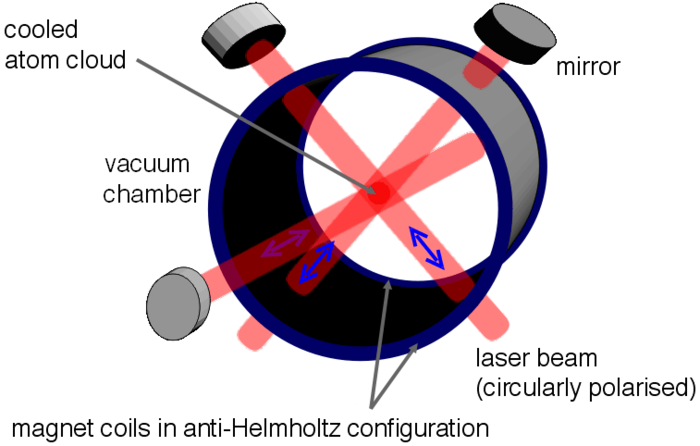
\includegraphics[width=0.75\textwidth]{images/MOT}
	\caption{From Wikipedia}
\end{figure}

Magneto-optical traps use a combination of red-detuned, circularly polarized, counter-propagating lasers, and a quadrupole magnetic field to trap neutral atoms with admissible atomic structure (i.e. not all atomic species can be magneto-optically trapped). \\


A theoretical description of a MOT is as follows. First, we require a vacuum and two coils in an anti-Helmholtz configuration. We let the coils be separated along the $z$-axis. To first order approximation (i.e. near the center), the magnetic field takes the form
\begin{equation*}
\vec{B} = B_0 \lp \f{x}{2}, \f{y}{2}, -z \rp, \quad B_0 = -\f{3\mu_0 I a R^2}{2(R^2 + a^2)^{5/2}}
\end{equation*}
where $R$ is the (common) radius of the coils and $2a$ is the distance between two coils. From here, we see that field strength is linear in position, and that the field gradient is twice as strong along the $z$ direction than along $x$ or $y$. 


\begin{figure}[!htb]
	\centering
	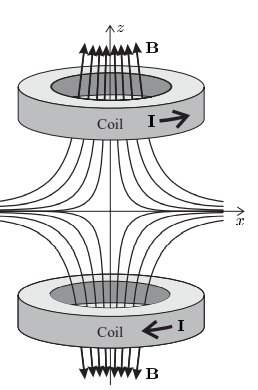
\includegraphics[width=0.4\textwidth]{images/anti-helmholtz}
	\caption{From \cite{foot2005atomic}.}
\end{figure}

Consider an atom with ground and excited states with $J=0$ and $J=1$, respectively. The Zeeman effect due to the magnetic field lifts the degeneracy in the $m_J$'s. For $J=1$ there are now $2J+1 = 3$ nondegenerate sublevels. For $J=0$ there is no such splitting. Since the magnetic field varies in space, the Zeeman effect on the atoms also varies in space, being more extreme for atoms further away from the center of the trap. \\


Next, we add three pairs of counter-propagating circularly-polarized orthogonal laser beams. The lasers are red-detuned from the $J=0 \to J=1$ transition. Circular polarization is required because we only want to selectively drive transitions from $\ket{0,0}$ to a specific $\ket{1,m_J}$ depending on where the atom is in the magnetic field. \\


When the atoms are the center of the trap, they don't experience any Zeeman shift and don't see the red-detuned light (not very much). They are the coldest and darkest atoms.\\


For an atom moving in the $+z \neq 0$ direction, for instance, the Zeeman effect shifts the energy of $\ket{J=1,m_F=-1}$ down closer to the energy of $\ket{J=0,m_J=0}$. In the $z$ direction, there are also the counter-propagating $\sigma^-$ and $\sigma^+$ in the $- z$ and $+z$ directions, respectively. Due to the Doppler effect, the atom moving in the $+z$ direction gets closer to resonance with the $\sigma^-$ beam traveling in the $-z$ direction, which drives the $\Delta m_J = -1$ transition, and feels a stronger scattering force the further it moves away from the center. When the atom absorbs a $\sigma^-$ photon, it goes to the $\ket{J=1,m_F=-1}$ state and gets a momentum kick opposite to its motion. It will eventually re-emits the photon due to spontaneous emission, but since the process is random and averages out to zero we see the atom affected mostly by the absorption of the $\sigma^-$ photon. The net effect is that the atom is pushed towards the center of the trap. Similarly, the atom moving the $-z$ direction is also pushed towards the center. The same thing happens in the $x-$ and $y-$directions.  
 	
 	
\begin{figure}[!htb]
	\centering
	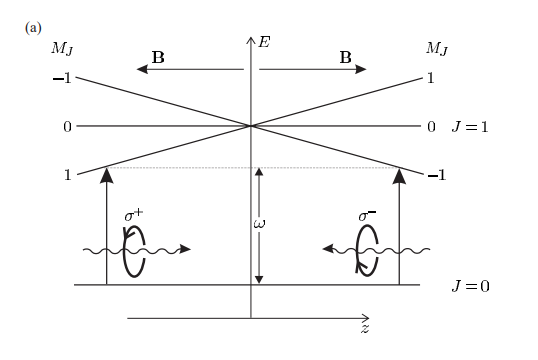
\includegraphics[width=0.75\textwidth]{images/foot_1}
	\caption{From \cite{foot2005atomic}}
\end{figure}

\begin{figure}[!htb]
	\centering
	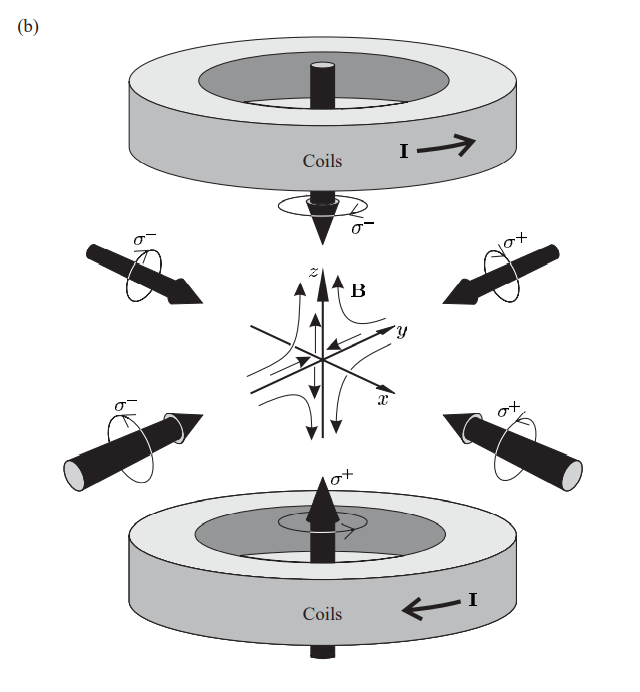
\includegraphics[width=0.7\textwidth]{images/foot_2}
	\caption{From \cite{foot2005atomic}}
\end{figure}


%%%%%%%%%%%%%%%%%%%%%%%%%%%%%%%%%%%%%%%
\chapter*{N}
%%%%%%%%%%%%%%%%%%%%%%%%%%%%%%%%%%%%%%%
\chapter*{O}



\section*{Optical lattice}



Optical lattice is one of those things which you think you know how they work but turns out that you don't. There are actually a number of technical details experimentalists must overcome in order to successfully trap atoms in a lattice. \\




An optical lattice is formed by the interference of counter-propagating laser beams, creating a spatially periodic \textbf{polarization} (or \textbf{intensity}) pattern. Atoms are cooled and localized in the potential minima (maxima) for red (blue) detuned light. The laser used is often far detuned.  The potential is due to the Stark effect; it is proportional to the laser intensity. \\

The energy shift to (and thus the potential experienced by) an electronic ground state $\ket{g_i}$ is given by second-order time-independent perturbation theory where the rapid time variation of the lattice potential at optical frequencies has been time-averaged:
\begin{equation*}
U(\mathbf{r}) = \Delta E_i = \f{3\pi c^2 \Gamma}{2\omega_0^3}\I(\mathbf{r}) \times  \sum_j \f{c_{ij}^2}{\Delta_{ij}}
\end{equation*}
where $\mu_{ij} = \bra{e_j}\mu \ket{g_i}  = \bra{e_j} \mathbf{d}\cdot \mathbf{E} \ket{g_i} \equiv c_{ij}\norm{\mu}$ are the transition matrix elements $\ket{g_i} \to \ket{e_j}$. For two-level atoms, this simplifies to 
\begin{equation*}
U(\mathbf{r}) = \Delta E = \f{3\pi c^2}{2\omega_0^3}\f{\Gamma}{\Delta} I(\mathbf{r}).
\end{equation*}
Here, $\Gamma$ is the natural linewidth of the excited state transition, i.e. the decay rate of spontaneous emission. 



\begin{framed}
	\noindent \textbf{Derivations of some results:}\\
	
	\noindent To see how we obtained the results above, let us go through the derivation given by \cite{grimm2000optical}. The article focuses on optical dipole trap, but the principle of operation transfer over exactly for optical lattices. The only major difference between the two trapping schemes is that the intensity of an optical lattice has a much more dramatic spatial variation than a standard optical dipole trap.\\
	
	Consider an atom placed in laser light. The laser light has electric field $\mathbf{E}$ oscillating at angular frequency $\omega$ which induces an atomic dipole moment $\mathbf{p}$. $\mathbf{p}$ also oscillates at $\omega$. If $\mathbf{E}(\mathbf{r},t) = \widehat{\epsilon} \widetilde{E}(\mathbf{r}) e^{-i\omega t} + c.c.$ then $\mathbf{\mathbf{p}}(\mathbf{r},t)  = \widehat{\epsilon} \widetilde{p}(\mathbf{r}) e^{-i\omega t} + c.c.$. Here $\widehat{\epsilon}$ denotes the unit polarization vector. The dipole amplitude $\widehat{p}$ is related to the amplitude of the electric field $\widetilde{E}$ by 
	\begin{equation*}
	\widetilde{p} = \al \widetilde{E}
	\end{equation*}
	where $\al$ is the (complex) polarizability, which depends on $\omega$. \\
	
	
	The \textbf{time-averaged interaction (dipole) potential} is given by the time-average of the dot product between $\mathbf{p}$ and $\mathbf{E}$:
	\begin{equation*}
	U_\text{dip} = -\f{1}{2} \langle \mathbf{p} \mathbf{E} \rangle = \dots = -\f{1}{2\epsilon_0 c} \Re(\al) I(\mathbf{r})
	\end{equation*}
	where $I = 2\epsilon_0 c^2 \abs{\widetilde{E}}^2$ is the intensity of the laser. The factor of $1/2$ takes into account the fact that the dipole is induced and not a permanent one. \\
	
	
	The \textbf{dipole force} is simply the negative gradient of the potential. We note now that the force is time-independent, as the time component of $U$ has already been averaged out:
	\begin{equation*}
	F_\text{dip}(\mathbf{r}) = -\nabla U_\text{dip}(\mathbf{r}) = \f{1}{2\epsilon_0 c}\Re(\al) \nabla I(\mathbf{r}). 
	\end{equation*}
	It is easy to see that the force is proportional to the intensity of the light. \\
	
	Next we want to calculate the atomic polarizability. To do this, we consider an atom in Lorentz's model of a classical oscillator and view the electron as a damped, driven harmonic oscillator whose position satisfies the following differential equation:
	\begin{equation*}
	\ddot{\mathbf{r}} + \Gamma_\omega \dot{\mathbf{r}} + \omega_0^2 \mathbf{r} = -\f{eE(t)}{m_e}.
	\end{equation*}
	Here, the electronic is considered to be bounded elastically to the core with a natural oscillation frequency $\omega_0$. The driving field is $E(t)$ with frequency $\omega$. $\Gamma_\omega$ is the damping rate, which results from the dipole radiation of the oscillating electron according charge acceleration (see Larmor's formula and \cite{jackson1999classical}). \\
	
	Solving this equation gives the amplitude of oscillation in terms of the driving frequency $\omega$
	\begin{equation*}
	\mathbf{r}(\omega) = \f{1}{m_e}\f{-eE(t)}{[(\omega_0^2 - \omega^2) + \Gamma_\omega^2 \omega^2]^{1/2}} =?= \f{1}{m_e} \f{-eE(t)}{(\omega_0^2 - \omega^2) - i\Gamma_\omega \omega}
	\end{equation*}
	 The second equality is not really an equality but rather the complex version of the solution. We can ignore that, as it's only a convention thing. The ``real'' solution is given in the first equality. \\
	 
	 Now recall that the dipole moment is related to $\mathbf{r}$ via $\mathbf{p} = -e\cdot \mathbf{r}$. So we can calculate $\mathbf{p}$. And finally, the polarizability $\al(\omega)$ is given by (as above): $\mathbf{p}(\omega) = \al(\omega) \mathbf{E}(\omega)$. So we have
	 \begin{equation*}
	 \al = \f{e^2}{m_e} \f{1}{\omega_0^2 - \omega^2 - i\omega \Gamma_\omega}.
	 \end{equation*}
	 From Larmor's formula for power radiated by an oscillating charge, we find 
	 \begin{equation*}
	 \Gamma_\omega = \f{e^2 \omega^2}{6\pi \epsilon_0 m_e c^3} \implies \f{e^2}{m_e} = \f{6\pi \epsilon_0 c^3 \Gamma_\omega}{\omega^2}.
	 \end{equation*}
	 Further, we introduce the on-resonance damping rate $\Gamma \equiv \Gamma_{\omega_0} =  (\omega_0/\omega)^2 \Gamma_\omega$. Putting everything together, we have
	 \begin{equation*}
	 \al = 6\pi \epsilon_0 c^3 \f{\Gamma/\omega_0^2}{\omega_0^2 - \omega^2 - i(\omega^3 / \omega_0^2) \Gamma}.
	 \end{equation*}
	 
	 
	 In general, the on-resonance damping rate $\omega$ cannot be calculated from Larmor's formula as this is classical theory. From the semi-classical approach, what one finds is that $\Gamma$ corresponds to the decay rate due to spontaneous emission: 
	 \begin{equation*}
	 \Gamma = \f{\omega_0^3}{3\pi \epsilon\hbar c^^3}\abs{\bra{e} \mu \ket{g}}^2.
	 \end{equation*}
	 
	 
	 
	 In any case, with this expression for the polarizability $\al$, we can write down the dipole interaction potential in terms of $\Gamma$ and frequencies:
	 \begin{equation*}
	 U_\text{dip}(\mathbf{r}) = -\f{3\pi c^2}{2\omega_0^3}\lp \f{\Gamma}{\omega_0 - \omega} + \f{\Gamma}{\omega_0 + \omega} \rp I(\mathbf{r}).
	 \end{equation*}
	 In the rotating wave approximation, the potential simplifies to 
	 \begin{equation*}
	 U_\text{dip}(\mathbf{r}) = +\f{3\pi c^2}{2\omega_0^3}\f{\Gamma}{\Delta} I(\mathbf{r}) 
	 \end{equation*}
	 where $\Delta$ is the detuning from the eigenfrequency of the electron in the Lorentz model. It turns out that (we will show this but won't prove) the \textbf{scattering rate} $\Gamma_\text{sc}$ is related to $U_\text{dip}$ via
	 \begin{equation*}
	 \hbar \Gamma_\text{sc} = \f{\Gamma}{\Delta} U_\text{dip}. 
	 \end{equation*}
	 The ``scattering'' process here can be thought of as due to viewing light as a stream of $\hbar \omega$ photons absorbed by the atom and re-emitted via spontaneous emission. \\
	 
	 
	 \noindent \textbf{Dipole trap potential and energy shift correspondence:}\\
	 
	 \noindent To find energy shifts to the oscillating electric field, we can make use of perturbation theory. Now, since the electric field is sinusoidal, the first-order correction to the energies will be zero by time-averaging. However, the second-order term may not be. In fact, we may very well expect the correction to energies to be non-zero in the second-order perturbation because this perturbation is proportional to the field \textit{intensity}, which is the square of the field. In any case, second-order perturbation theory (for non-degenerate states) says that
	 \begin{equation*}
	 \Delta E_i = \sum_{j\neq i} \f{\abs{\bra{j} \ham'\ket{i}}^2}{E_i - E_j}
	 \end{equation*} 
	 where we have perturbation Hamiltonian $\ham' = e \mathbf{r}\cdot \mathbf{E} $ and $E_i - E_j = \hbar \Delta_{ij}$. For a two-level system (which is what we are considering now), the energy shift turns into
	 \begin{equation*}
	 \Delta E = \pm \f{\abs{\bra{e} e\mathbf{r} \ket{g}}^2}{\hbar \Delta_{ij}} \abs{E}^2 = \pm \f{3\pi c^2}{2\omega_0^3} \f{\Gamma}{\Delta}I(\mathbf{r}) = \pm U_\text{dip}(\mathbf{r}).  
	 \end{equation*}
	 Here, the ground state is shifted down and excited state is shifted up, each by $\Delta E$, if $\Delta < 0$ (red-detuned).  \\
	 
	 We see that the optically induced light shift, i.e., the \textbf{ac Stark shift} of the ground-state energy \textbf{corresponds exactly} to the \textbf{dipole potential} for the two-level atom. \\
	 
	 
	 
	 For multi-level atoms, we will have a collection of dipole matrix elements $\mu_{ij} = \bra{e_i}\mu\ket{g_j}$, which can be written in terms of a reduced matrix element $\norm{\mu}$ multiplied by some transition coefficient $c_{ij}$ which one can look up in some table. From standard quantum mechanics, one may find that the fully reduced matrix element only depends on the orbital wave functions and is directly related to the spontaneous emission decay rate. In any case, the energy shift now takes the form
	 \begin{equation*}
	 \Delta E_i = \f{3\pi c^2 \Gamma}{2\omega_0^3} I \times \sum_j \f{c_{ij}^2}{\Delta_{ij}}.
	 \end{equation*}
	 
	 
	 On the basis of this equation  one can derive a general result for the potential of a ground state with total angular momentum F and magnetic quantum number mF , which is valid for both linear and circular polarization as long as all optical detunings stay large compared with the
	 excited-state hyperfine splitting. We won't go into that here, but the reader is welcomed to refer to \cite{grimm2000optical} for more details. 
\end{framed}


\begin{figure}[!htb]
	\centering
	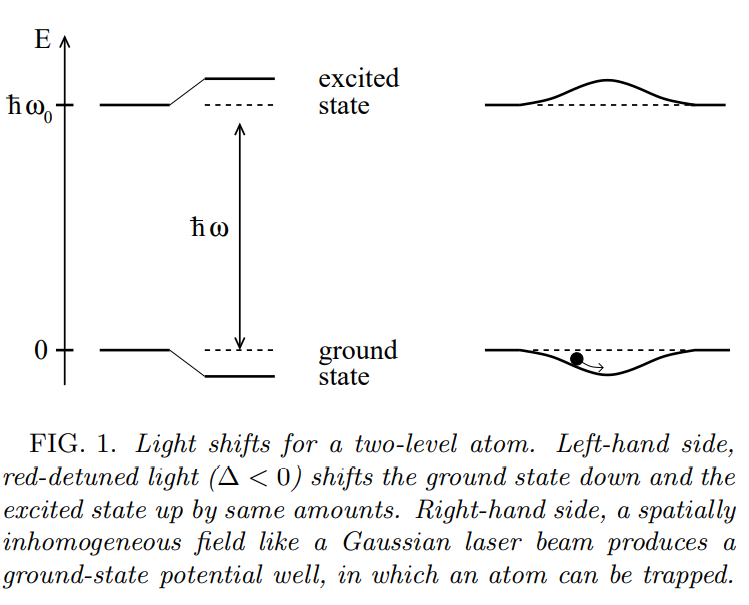
\includegraphics[width=0.5\textwidth]{images/dipole_trap}
	\caption{From \cite{grimm2000optical}}
\end{figure}


Atoms trapped in the potential wells may still move across wells even if the well depth exceeds the kinetic energies of the atoms. This is due to quantum tunneling. However, a \textbf{superfluid-Mott insulator transition} may occur when the interatomic interaction is sufficiently strong. (stronger than the well depth). In the Mott insulator phase, the atoms are trapped at the potential minima/maxima and cannot move freely (hence ``insulator''). \\


There are two parameters for an optical lattice: the potential well depth and the periodicity of the lattice. The potential experienced by the atoms (note that the potential is felt only by the atoms because of the Stark shift -- inherent to the atoms) depends on the intensity of the laser used to generate the optical lattice. The intensity of this laser is usually controlled by an AOM. The periodicity of an optically lattice can be tuned by changing the wavelength of the laser used or by changing the relative angle between the laser beams. 






\section*{Optical dipole trap}


\section*{Optical tweezer}


%%%%%%%%%%%%%%%%%%%%%%%%%%%%%%%%%%%%%%%
\chapter*{P}



\section*{PID Controller (basics)}


\subsection*{OpAmps}


\subsection*{PID controller}




%\section*{Perturbation theory in QM (simple version)}





\section*{Pound-Drever-Hall (PDH) technique}
%%%%%%%%%%%%%%%%%%%%%%%%%%%%%%%%%%%%%%%
\chapter*{Q}

\section*{Quantum Harmonic Oscillator}

This is one of the most important concepts in quantum mechanics that is applied almost all the time in AMO physics, so it is \textit{very} good to know. \\


In one dimension, the Hamiltonian is given by 
\begin{equation*}
\widehat{H} = \f{\widehat{p}^2}{2m} + \f{1}{2}k\widehat{x}^2 =  \f{\hat{p}^2}{2m} + \f{1}{2}m\omega^2 \widehat{x}^2,
\end{equation*}
where $m$ is the particle mass, $\omega = \sqrt{k/m}$ is the angular frequency of the particle, and $\widehat{x}$ and $\widehat{p}$ are the position and momentum operators, respectively. The wavefunction of the particle satisfies the time-independent SE says $\widehat{H}\ket{\psi} = E\ket{\psi}$. In position space, the solution space for $\widehat{H}$ is spanned by the following Hermite functions
\begin{equation*}
\bra{x}\ket{\psi} = \psi_n = \f{1}{\sqrt{2^n n!}} \lp \f{m\omega}{\pi \hbar} \rp^{1/4} e^{-m\omega^2 x/2\hbar} H_n\lp \f{\sqrt{m\omega}}{\hbar} x \rp
\end{equation*}
where $n \in \mathbb{N}$ and $H_n$ are Hermite polynomials. The corresponding energy levels are 
\begin{equation*}
E_n = \hbar \omega \lp n + \f{1}{2} \rp,
\end{equation*}
and so the zero-point energy is $\hbar\omega/2$, which is non-zero due to the Heisenberg uncertainty principle. We notice that the energies are quantized and adjacent levels are equally spaced by one unit of $\hbar\omega$. We note also that when the \textcolor{blue}{harmonicity} of the potential is lost, we are no longer guaranteed equal spacings between adjacent levels. \\


One way to solve the QHO problem is by using ladder operators (so that we avoid Hermite functions, etc.). We define the creation and annihilation operators as below:
\begin{equation*}
\widehat{a}^\dagger = \sqrt{\f{m\omega}{2\hbar}} \lp \widehat{x} - \f{i}{m\omega}\widehat{p} \rp, \quad \widehat{a} = \sqrt{\f{m\omega}{2\hbar}} \lp \widehat{x} + \f{i}{m\omega}\widehat{p} \rp
\end{equation*}
from which we can represent the position and momentum operators as 
\begin{equation*}
\widehat{x} = \sqrt{\f{\hbar}{2m\omega}} (\widehat{a}^\dagger + \widehat{a}), \quad \widehat{p} = i\sqrt{\f{\hbar m\omega}{2}}(\widehat{a}^\dagger - \widehat{a}).
\end{equation*}
Creation and annhilation operators are not Hermitian. Rather, they are idempotents. They act on the energy eigenstates the following way:
\begin{equation*}
\widehat{a}\ket{n} = \sqrt{n}\ket{n-1}, \quad a\ket{0} = 0, \quad \widehat{a}^\dagger\ket{n} = \sqrt{n+1}\ket{n+1}.
\end{equation*}
This explains why these operators are called the way they are. The number operator $\widehat{N}$ can be defined from the ladder operators:
\begin{equation*}
\widehat{N}\ket{n} \equiv \widehat{a}^\dagger \widehat{a}\ket{n} = n\ket{n}, 
\end{equation*}
and so 
\begin{equation*}
\widehat{H} = \hbar\omega\lp \widehat{a}^\dagger \widehat{a} + \f{1}{2} \rp = \hbar\omega \lp \widehat{N} + \f{1}{2} \rp.
\end{equation*}
With these definitions, one can express any excited state in terms of the ground state:
\begin{equation*}
\ket{n} = \f{(\widehat{a}^\dagger)^n}{\sqrt{n!}} \ket{0}.
\end{equation*}
The QHO can be easily generalized to an $N$-dimensional isotropic QHO by simply repeating the 1D problem $N$ times. The energy is given by 
\begin{equation*}
E = \hbar\omega\lp n_1 + n_2 + \dots + n_N + \f{N}{2} \rp.
\end{equation*}



%%%%%%%%%%%%%%%%%%%%%%%%%%%%%%%%%%%%%%%
\chapter*{R}



\section*{Rabi frequency}


The Rabi frequency is defined as 
\begin{equation*}
\Omega_{ij} = \f{\vec{d}_{ij}\cdot \vec{E}_0}{\hbar}
\end{equation*}
where $\vec{d}_{ij}$ is the transition dipole moment for the $i\to j$ transition, $\vec{E}_0 = \hat{\epsilon} E_0$ is the vector electric field amplitude which includes the polarization. $\Omega_{ij}$ has units of angular frequency. \\


The Rabi frequency is the frequency of fluctuations in the populations of the two atomic levels involved in the atomic transition being considered. It is proportional to the strength of the coupling between the light and the atomic transition (dipole moment) and to the amplitude of the light's electric field. \\


When light is exactly resonant with the transition, Rabi flopping (the fluctuation in populations of the ground and excited states) occurs at the Rabi frequency. When light is detuned from resonance, then Rabi flopping occurs at the generalized Rabi frequency, given by 
\begin{equation*}
\widetilde{\Omega}_{ij} = \sqrt{\abs{\Omega_{ij}}^2 + \Delta^2}
\end{equation*}
where $\Delta$ is the detuning. Further, as light is more detuned from resonance, the amplitude of Rabi oscillations decreases. \\


Everything is characterized by the Rabi formula, which gives the population of the excited state $\ket{1}$ at time $t$, when the system is originally in state $\ket{0}$:
\begin{equation*}
P_{0\to 1}(t) = \f{\abs{\Omega}^2}{\Delta^2 + \abs{\Omega}^2}\sin^2\lp \f{\sqrt{\abs{\Omega}^2 + \Delta^2}}{\hbar} t \rp
\end{equation*}
Here, $\sqrt{\abs{\Omega}^2 + \Delta^2}$ is the generalized Rabi frequency and $\Omega$ is the Rabi frequency, which appears in the two-level Hamiltonian as
\begin{equation*}
\ham = 
\begin{pmatrix}
E + \Delta & \Omega \\ \Omega^* & E - \Delta
\end{pmatrix}.
\end{equation*}






\section*{Raman scattering}




\section*{Raman cooling}

Raman cooling is a sub-Doppler/recoil cooling technique. The general mechanism is as follows. Consider a collection of atoms with two hyperfine states. The transition between these two states is triggered by two laser beams: the first beam excites the atoms to some virtual excited state, and the second beam deexcites (via stimulated emission) the atoms to the other hyperfine level. The frequency difference between the two beams is equal to the spacing between the hyperfine levels. This is the general Raman process.


\begin{figure}[!htb]
	\centering
	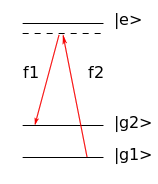
\includegraphics[width=0.25\textwidth]{images/raman}
	\caption{From Wikipedia}
\end{figure}


Now we use the general Raman process to do free-space Raman cooling. In this scheme, pre-cooled atoms experience pulses of Raman-like processes. The two laser beams in this case are now counter-propagating, with $f_2$ being red-detuned with respect to its normal value. This allows for atoms moving towards the $f_2$ beam to be slowed down due to the Doppler effect and end up in the state $\ket{g_2}$. By regularly exchanging the propagation direction of the laser beams and varying the (red) detuning, we can get \textbf{all} atoms whose initial velocities satisfying $\abs{v} > v_\text{max}$ to be in the state $\ket{g_2}$, while atoms with $\abs{v} < v_\text{max}$ remain in the $\ket{g_1}$ state. \\

Now, we need to slow down the atoms in $\ket{g_2}$. To do this, a new beam whose frequency is exactly the spacing between $\ket{g_2}$ and $\ket{e}$ is switched on. This beam optically pumps the atoms from $\ket{g_2}$ to $\ket{g_1}$, and the velocities will be randomized in this process and so inevitably a fraction of the atoms in $\ket{g_2}$ will acquire speeds $\abs{v} < v_\text{max}$. By repeating this process several times, the temperature of the cloud can be reduced (to lower than a microkelvin.)\\


For more information about this technique and its working principle, the reader may refer to \cite{PhysRevLett.69.1741}.








\section*{Raman side-band cooling}

Raman side-band cooling is a sub-technique of Raman cooling. This cooling technique starts from atoms in a MOT, with an optical lattice present. We assume that the optical lattice is sufficiently deep that each site is essentially a harmonic trap. Since the atoms are not in the their ground state, they will be trapped in one of the excited levels of the quantum harmonic oscillator. Raman side-band cooling aims to bring these atoms to the ground state of the harmonic potential at each site, and it requires access to the atomic structure of the atoms. \\


Suppose the atom has two levels with ground state $F=1$, such that there is a three-fold degeneracy $m_F = -1,0,1$. A magnetic field is added to induce Zeeman shifts, lifting the degeneracy. The magnetic field strength is tuned such that the Zeeman splitting between the $\Delta m_F = 1$ states matches the spacing of the two levels in the harmonic potential.


\begin{figure}[!htb]
	\centering
	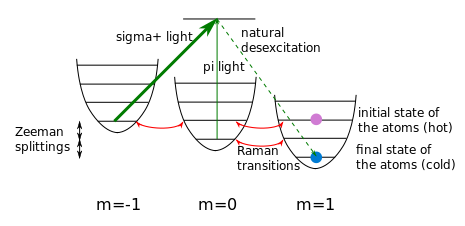
\includegraphics[width=0.75\textwidth]{images/raman_sideband}
	\caption{From Wikipedia}
\end{figure}


By Raman processes, one can transfer an atom to a state whose $m_F$ and vibrational state has changed by $-1$. After all this, the atoms in the lowest vibrational state of the harmonic trap, except for those with $m_F = 1$, are optically pumped to the $m_F = 1$ state using $\sigma_+$ and $\pi$ light. 






\section*{Recoil temperature}

Consider an atom undergoing spontaneous emission of a single photon whose momentum is $p = \hbar k = h/\lambda$. By momentum conservation, the momentum kick that the atom gains is also $p$, and its kinetic energy is $p^2/2m = \hbar^2k^2/2m$. The recoil temperature is given by 
\begin{equation*}
T_r = \f{\hbar^2k^2}{k_Bm} = \f{h^2}{k_B m \lambda^2}.
\end{equation*} 
There is a factor of $1/2$ in an alternative definition, which can be obtained from setting $T_r k_B = p^2/2m$. But I'm following the convention set by \cite{metcalf2007laser}, which does not include the factor of $1/2$.






\section*{Rotating wave approximation}


The rotating wave approximation ignores highly oscillatory terms in the Hamiltonian. This is a valid approximation when the applied electromagnetic radiation is near resonance with an atomic transition, and the intensity is low. The name of the approximation comes from the transformation of the Hamiltonian to the \textbf{interaction picture}. In this picture, the atomic Hamiltonian is absorbed into the system ket, and so the evolution due to the interaction with the atom with the light field is the only thing to consider. \\


Consider a example of a two-level system with resonance frequency $\omega_0$. The atomic Hamiltonian is 
\begin{equation*}
\ham_0 = \f{\hbar \omega_0}{2}\ket{e}\bra{e} - \f{\hbar\omega_0}{2}\ket{g}\bra{g}.
\end{equation*}
Now we introduce a classical electric field $\vec{E}(t) = \vec{E}_0 e^{-i\omega_L t} + \vec{E}_0^* e^{+i \omega_L t}$. Under the \textbf{dipole approximation}, the interaction Hamiltonian is given by 
\begin{equation*}
\ham_I = -\vec{d} \cdot \vec{E},
\end{equation*}
where $\vec{d}$ is the dipole moment operator of the atom. To go further, we have to find the matrix elements of $\vec{d}$. Notice that $\bra{e} \vec{d} \ket{e} = \bra{g}\vec{d}\ket{g} = 0$ due to parity. So, we only have the matrix element $\bra{e} \vec{d} \ket{g}$ and its complex conjugate. Let $\vec{d}_{eg} = \bra{e} \vec{d} \ket{g}$, then $\vec{d}$ is just 
\begin{equation*}
\vec{d} = \vec{d}_{eg} \ket{e}\bra{g} + \vec{d}_{eg}^* \ket{g}\bra{e}. 
\end{equation*}
With this, the interaction Hamiltonian becomes:
\begin{align*}
\ham_1 
&=  -\vec{d}\cdot \vec{E}\\
&= - \lp \vec{d}_{eg} \ket{e}\bra{g} + \vec{d}_{eg}^* \ket{g}\bra{e} \rp
 \cdot \lp \vec{E}_0 e^{-i\omega_L t} + \vec{E}_0^* e^{+i \omega_L t} \rp\\
&= - \lp \vec{d}_{eg}\cdot \vec{E}_0 e^{-i\omega_L t} + \vec{d}_{eg}\cdot \vec{E}_0^* e^{+i\omega_L t} \rp \ket{e}\bra{g}\\
&\quad\quad - \lp \vec{d}_{eg}^*\cdot \vec{E}_0 e^{-i\omega_L t} + \vec{d}_{eg}^*\cdot \vec{E}_0^* e^{+i\omega_L t} \rp \ket{g}\bra{e}\\
&= -\hbar \lp \Omega e^{-i\omega_L t} + \widetilde{\Omega}^*e^{+i\omega_L t} \rp \ket{e}\bra{g} - \lp \widetilde{\Omega}^* e^{-i\omega_L t} + \Omega e^{+i\omega_L t} \rp \ket{g}\bra{e}.
\end{align*}

The Hamiltonian in the interaction picture is obtained by the unitary transform $\ham_{1,I} = U \ham_1 U^\dagger$ where
\begin{equation*}
U = e^{i \ham_0 t/\hbar} = \ket{g}\bra{g} + e^{i\omega_0 t}\ket{e}\bra{e}.
\end{equation*}
So we have
\begin{align*}
\ham_{1,I} &= U \ham_1 U^\dagger\\
&= -\hbar \lp \Omega e^{-i\Delta t} + \widetilde{\Omega}^*e^{+i(\omega_L + \omega_0) t} \rp \ket{e}\bra{g} - \hbar\lp \widetilde{\Omega}^* e^{-i(\omega_L  + \omega_0)t} + \Omega e^{+i\Delta t} \rp \ket{g}\bra{e}
\end{align*}
where $\Delta = \omega_L - \omega_0$ is the detuning and $\omega_L + \omega_0$ is the high frequency which we want to eliminate. Here is where the rotating approximation comes in: 
\begin{equation*}
\ham_{1,I}^{\text{RWA}} = -\hbar \Omega e^{-i\Delta t}  \ket{e}\bra{g} - \hbar\Omega e^{+i\Delta t}  \ket{g}\bra{e}.
\end{equation*} 
Transforming this back into the Schr\"{o}dinger picture we have
\begin{align*}
\ham_1^\text{RWA} &= U^\dagger\ham_{1,I}^{\text{RWA}}U \\
&= -\hbar \Omega e^{-i\Delta t}e^{-i \omega_0 t}\ket{e}\bra{g} - \hbar \Omega^* e^{i\Delta t}\ket{g}\bar{e}e^{i\omega_0 t}\\
&= -\hbar \Omega e^{-i\omega_L t}\ket{e}\bra{g} - \hbar \Omega^* e^{i\omega_L t}\ket{g}\bra{e}.
\end{align*}
The total Hamiltonian in the rotating wave approximation is thus
\begin{align*}
\ham^\text{RWA} &= \ham_0+ \ham_1^\text{RWA} \\
&= \f{\hbar \omega_0}{2}\ket{e}\bra{e} - \f{\hbar \omega_0}{2}\ket{g}\bra{g} -\hbar \Omega e^{-i\omega_L t}\ket{e}\bra{g} - \hbar \Omega^* e^{i\omega_L t}\ket{g}\bra{e}.
\end{align*}
In the standard basis, we have
\begin{equation*}
\ham^\text{RWA} =  \f{\hbar}{2} \begin{pmatrix}
\omega_0 & -\Omega e^{-i\omega_L t} \\ -\Omega^* e^{i\omega_L t} & -\omega_0
\end{pmatrix}.
\end{equation*}






%%%%%%%%%%%%%%%%%%%%%%%%%%%%%%%%%%%%%%%
\chapter*{S}




%\section*{Sisyphus cooling}


%\section*{Stark effect}


%\section*{Standing waves (Energy and Polarization)}






\section*{Superexchange in optical lattice}


Consider a double-well potential with two Bosonic spins, where the relative depths of the wells can be tuned. There are four possible configurations for the system: $\ket{\uparrow, \downarrow}, \ket{\uparrow\downarrow,0}, \ket{0,\uparrow\downarrow}, \ket{\downarrow, \uparrow}$, where the spin on left denotes the spin on the left well, and the spin on the right denotes the spin on the right well. The states $\ket{\uparrow,\downarrow}$ and $\ket{\downarrow,\uparrow}$ are degenerate, and the states $\ket{\uparrow\downarrow,0}$ and $\ket{\downarrow\uparrow,0}$ are separated by $2\Delta$, where $\Delta$ is the difference between the well depths. These two manifolds of states are separated by the interatomic interaction energy $U \gg \Delta$.  Due to quantum tunneling, the manifolds are also coupled, via the tunneling term $J$. We are interested in the \textcolor{blue}{superexchange coupling} $J_{\text{ex}}$ between the states $\ket{\uparrow,\downarrow}$ and $\ket{\downarrow, \uparrow}$. 



\begin{figure}[!htb]
	\centering
	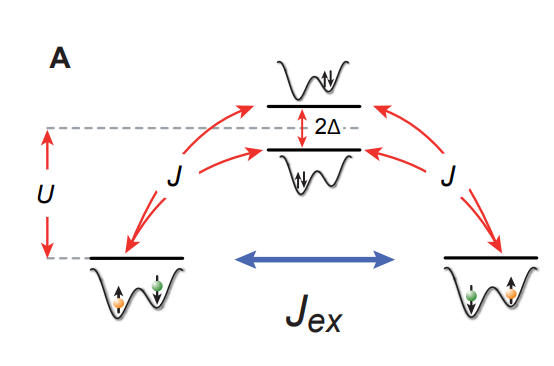
\includegraphics[width=0.75\textwidth]{images/superex_1}
	\caption{From \cite{trotzky2008time}}
\end{figure} 

The system can be described by a two-site version of the Bose-Hubbard Hamiltonian:
\begin{equation*}
\widehat{H}= \sum_{\sigma = \uparrow,\downarrow}\lb -J\lp \widehat{a}^\dagger_{\sigma L}\widehat{a}_{\sigma R} + \widehat{a}^\dagger_{\sigma R}\widehat{a}_{\sigma L} \rp  - \Delta(\widehat{n}_{\sigma L} - \widehat{n}_{\sigma R} )  \rb + U\lp \widehat{n}_{\uparrow L} \widehat{n}_{\downarrow L} + \widehat{n}_{\uparrow R}\widehat{n}_{\downarrow R} \rp
\end{equation*}
This Hamiltonian makes sense: it says that the strength of the hopping (tunneling, i.e., annihilating in one well and appearing in the other) between the wells is $J$. The second term says that the potential bias is $\Delta$: we see that indeed $\ket{\uparrow,\downarrow}$ has the same energy as $\ket{\downarrow,\uparrow}$. But if there are two particles per site, then the difference between the number operators can be $\pm 2$, and the difference in energy between the states $\ket{\uparrow\downarrow,0}$ and $\ket{\downarrow\uparrow,0}$ is $2\Delta$. The last term tells us about the coupling between the $(1,1)$ and $(2,0)$ manifolds. This term assigns an energy of $0$ to the one-particle-per-site states, and assigns $U$ to the $(2,0)$ states. \\




Let's do a quick example. Assume that $\Delta = 0$ for now. In the basis $\{ 
\ket{\uparrow, \downarrow}, 
\ket{\uparrow\downarrow, 0}, 
\ket{0,\uparrow\downarrow}, 
\ket{\downarrow,\uparrow}\}$, the Hamiltonian is of the form
\begin{equation*}
\widehat{H} = \begin{bmatrix}
0 & -J & -J & 0\\
-J & U & 0& -J\\
-J & 0 & U & -J\\
0& -J &-J  & 0
\end{bmatrix}.
\end{equation*}
The eigenvalues associated with this Hamiltonian are 
\begin{equation*}
0, \quad U, \quad \text{ and }\quad \f{1}{2}\lp U \pm \sqrt{16 J^2+U^2} \rp. 
\end{equation*}
Redefining the zero energy (which doesn't change the dynamics of the Hamiltonian), we obtain the following energy diagram for the system (where $\Delta=0$):
\begin{figure}[!htb]
	\centering
	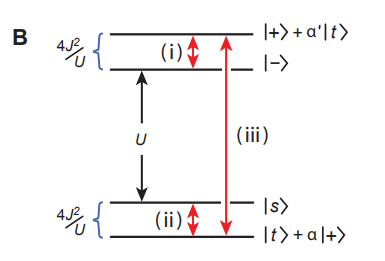
\includegraphics[width=0.7\textwidth]{images/superex_2}
	\caption{From \cite{trotzky2008time}}
\end{figure}





Here, we have Taylor expanded the last two eigenvalues under the assumption that $U\gg J$. The eigenstates of the system, from lowest to highest in energy, are
\begin{align*} 
\ket{t}+ \al\ket{+} &\propto \f{1}{\sqrt{2}}\lp \ket{\uparrow,\downarrow} + \ket{\downarrow,\uparrow} \rp + \f{J}{2U}\f{1}{\sqrt{2}}\lp \ket{\uparrow\downarrow,0}+ \ket{0,\uparrow\downarrow} \rp  \\
\ket{s} &= \f{1}{\sqrt{2}}\lp -\ket{\uparrow,\downarrow}+ \ket{\uparrow,\downarrow} \rp \\
\ket{-} &=  \f{1}{\sqrt{2}}\lp \ket{\uparrow\downarrow,0} - \ket{0,\uparrow\downarrow} \rp\\
\ket{+} + \al'\ket{t} &= \f{1}{\sqrt{2}}\lp \ket{\uparrow\downarrow,0} + \ket{0,\uparrow\downarrow} \rp - \f{2J}{U}\f{1}{\sqrt{2}}\lp \ket{\uparrow,\downarrow} + \ket{\downarrow,\uparrow} \rp.
\end{align*}

Since $J \ll U$, we see that the new eigenstates are small perturbations of $\ket{t},\ket{s},\ket{-},\ket{+}$, in that order. The states $\ket{t}+\al\ket{+}$ and $\ket{s}$ are spaced by $4J^2/U$, and similarly for $\ket{-}$ and $\ket{+}+ \al'\ket{t}$.  \\



By changing the bias $\Delta$, it is possible to create spin imbalances, spin oscillations, etc. 











%%%%%%%%%%%%%%%%%%%%%%%%%%%%%%%%%%%%%%%
\chapter*{T}
%%%%%%%%%%%%%%%%%%%%%%%%%%%%%%%%%%%%%%%
\chapter*{U}
%%%%%%%%%%%%%%%%%%%%%%%%%%%%%%%%%%%%%%%
\chapter*{V}
%%%%%%%%%%%%%%%%%%%%%%%%%%%%%%%%%%%%%%%
\chapter*{W}


\section*{WKB approximation}

The WKB method is used to find approximate solutions to the time-independent SE in 1D. It is particularly useful in calculating \textbf{bound state energies} and \textbf{tunneling rates} through potential barriers.  The contents of this section are from \cite{harrow8} and \cite{griffiths2018introduction}. \\



The WKB approximation is slightly different from perturbation theory. Perturbation theory covers the limits where $\delta H $ is small relative to $\abs{E_m^0 - E_n^0}$. The WKB approximation covers the limits where the system is close to being classical (which is why it is also called a \textit{semiclassical approximation}). It results in powers not of $\delta H$ but of $\hbar$, and thus becomes exact in the classical limit ($\hbar \to 0$). \\


Before we start, let's set up a few things. First, we have the \textbf{probability density function}
\begin{equation*}
\rho(\vec{x},t) = \abs{\psi (\vec{x},t)}^2.
\end{equation*} 
From the conservation of probability equation $\p_t P + \vec{\nabla}\cdot \vec{j} = 0$ (which follows from taking the time derivative of $P$ and applying the SE), where $j$ is the probability flux, given by 
\begin{equation*}
\vec{j}(\vec{x},t) = \f{\hbar}{2mi}\lb \psi^* \vec{\nabla} \psi - \psi \vec{\nabla} \psi^* \rb = \f{\hbar}{m} \Im \lp \psi^* \vec{\nabla} \psi \rp = \f{1}{m} \Re\lp \psi^* \widehat{p} \psi \rp
\end{equation*}
where $\widehat{p} = -i\hbar \vec{\nabla}$ is of course the momentum operator. \\



We see that if we write the wavefunction $\psi$ as
\begin{equation*}
\psi(\vec{x},t) = \sqrt{\rho(\vec{x},t)} e^{iS(x)/\hbar}
\end{equation*}  
where $S(x)$ is purely real, then by the definition of $\vec{j}$ we have
\begin{equation*}
\vec{j}(\vec{x},t) = \f{\hbar}{m} \Im\lp \psi^* \vec{\nabla} \psi\rp = \f{\hbar}{m} \f{\rho}{\hbar} \vec{\nabla}S. 
\end{equation*}
So, the phase function is related to the probability flux:
\begin{equation*}
\vec{j}(\vec{x},t) = \rho \f{\vec{\nabla}S }{m}.
\end{equation*}
We'll get back to these things later. \\



Consider a particle with energy $E$ and mass $m$ moving in a potential $V(x)$. Classically, the kinetic energy is $E - V(x)$. This suggests that the momentum can be defined by 
\begin{equation*}
p(x) = \sqrt{2m(E-V(x))} \implies \lambda_{\text{de Broglie}} = \f{h}{p(x)} = \f{2\pi \hbar}{p(x)}.
\end{equation*} 
We have the following DE:
\begin{equation*}
\hbar^2 \p_x^2 \psi = -2m(E-V(x)) \psi \equiv -\kappa^2 \psi. 
\end{equation*}
If $V(x) \leq E$ then we have exponentially decaying solutions ``at rate $\kappa(x)$.'' \\


Put $\psi(x) = e^{iS(x)/\hbar}$, where $S(x)$ is complex. Substituting this into the SE (for the classical region), we have
\begin{align*}
p^2(x) e^{iS(x)/\hbar} &= -\hbar^2 \p_x^2 e^{iS(x)\hbar} \\
&= -\hbar^2 \lp i \f{S''(x)}{\hbar}  - \f{(S'(x))^2}{\hbar}\rp e^{iS(x)/\hbar}
\end{align*}
which gives
\begin{equation*}
\boxed{(S')^2 - i\hbar S'' = p^2(x)},
\end{equation*}
where derivatives are with respect to $x$. So far this is exact, but here is where the WKB approximation comes in. If the potential $V(x)$ is slowly varying in $x$, then $p(x)$ is also slowly varying in $x$, and the $-i\hbar S''$ term will be small. Here, ``slowly varying'' means that the variation in the potential is across distances that are very large compared to de Broglie wavelength of the particle. In the classical limit, $\hbar$ is small, so we may write 
\begin{equation*}
S(x) = S_0(x) + \hbar S_1 (x) + \hbar^2 S_2(x) + \dots
\end{equation*}
The WKB approximation takes
\begin{equation*}
S(x) = S_0(x) + \hbar S_1(x). 
\end{equation*}
substituting this back into the boxed equation and eliminate higher order terms, we find 
\begin{equation*}
(S_0')^2 = p^2(x) \, \text{ at } \mathcal{O}(\hbar^0) \quad \text{and } \quad
2S_0'S_1' - iS_0'' = 0\, \text{ at } \mathcal{O}(\hbar^1).
\end{equation*}
The first equation gives
\begin{equation*}
S_0(x) = \pm  \int_{x_0}^x p(x')\,dx'
\end{equation*}
where $x_0$ is arbitrary, and by substituting this into the second equation, we find 
\begin{equation*}
S_1(x) = \f{i}{2} \ln p(x) + C.
\end{equation*}
With these, we can write down the approximate wavefunction:
\begin{align*}
\psi(\vec{x},t) = e^{iS(x)/\hbar} &\approx e^{i(S_0(x) + \hbar S_1(x))/\hbar}\\
&= \exp\lp \pm \f{i}{\hbar}\int_{x_0}^x p(x')\,x' \rp \exp \lp -\f{1}{2}\ln p(x) + C \rp
\end{align*}
Thus in the classically allowed regions we have the solution
\begin{equation*}
\boxed{\psi(\vec{x}) = \f{A}{\sqrt{\abs{p(x)}}} \exp\lp \f{i}{\hbar}\int_{x_0}^x p(x')\,x' \rp  + \f{B}{\sqrt{\abs{p(x)}}} \exp\lp -\f{i}{\hbar}\int_{x_0}^x p(x')\,x' \rp    }
\end{equation*}
with $p(x) = \sqrt{2m (E - V(x))}$. In the classically forbidden region, $p(x)$ becomes purely imaginary, and we have
\begin{equation*}
\boxed{\psi(\vec{x}) = \f{C}{\sqrt{\abs{p(x)}}} \exp\lp \f{1}{\hbar}\int_{x_0}^x\abs{ p(x')}\,x' \rp  + \f{D}{\sqrt{\abs{p(x)}}} \exp\lp -\f{1}{\hbar}\int_{x_0}^x \abs{p(x')}\,x' \rp    }
\end{equation*}
For some details about the validity of the WKB method, see \cite{harrow8}. \\



\subsection*{Bohr-Sommerfeld quantization}
WKB generalizes an idea in ``old quantum mechanics'' that quantum orbits are quantized by $h = 2\pi \hbar$. Consider an infinite well, with $V(x)$ finite (not necessarily constant) between $x=0$ and $x=a$ and infinite elsewhere. Assume that $E > V(x)$ for all  $0 < x < a$. The solution from WKB has the form 
\begin{equation*}
\psi(x) = \f{1}{\sqrt{p(x)}} (C\cos(\phi(x)) + D\sin(\phi(x))). 
\end{equation*}
where 
\begin{equation*}
\phi(x) = \f{1}{\hbar}\int_{0}^x p(x')\,dx'.
\end{equation*}
Since $\psi(0) = \phi(0) = 0$, we find $C =0$. From $\psi(a) = 0$ we find that $\phi(a) = n\pi$. So, we have a quantization condition:
\begin{equation*}
\f{1}{\hbar}\int_0^a \sqrt{2m (E_n - V(x))}\,dx = n\pi,
\end{equation*}
where $E_n$ is the $n$th energy level. \\

As a sanity check, we see that when $V =0 $ between $x = 0$ and $x=a$, we get the infinite square well energies:
\begin{equation*}
E_n = \f{\pi^2 \hbar^2 n^2}{2ma^2}
\end{equation*}




\subsection*{Connection formulae}
What if we have potential walls that are not hard vertical walls? For this we will need \textbf{connection formulae}  to connect oscillating solutions in the allowed regions with the decaying solutions in the forbidden regions. 


Let's look at what happens when we replace the infinite square well with a harmonic oscillator potential. The Hamiltonian in this case is 
\begin{equation*}
H = \f{p^2}{2m} + \f{1}{2} m \omega^2 x^2.
\end{equation*}

Recall that the energy levels are 
\begin{equation*}
E_n = \hbar \omega \lp n+ \f{1}{2} \rp. 
\end{equation*}
The turning point for each $\ket{n}$ is given by equating the potential and the energy:
\begin{equation*}
\f{1}{2}m\omega^2 x^2 = \hbar \omega \lp n+ \f{1}{2} \rp. 
\end{equation*}
This gives
\begin{equation*}
x_\text{turn} = \pm  \sqrt{\f{\hbar}{m\omega}} \sqrt{2n + 1}.
\end{equation*}
Repeating what we've done before, we have
\begin{equation*}
\phi(x) = \f{1}{\hbar}\int_{-x_\text{turn}}^{x_\text{turn}} p(x')\,dx' = \f{1}{\hbar}\int_{-x_\text{turn}}^{x_\text{turn}} \sqrt{2m(E - V(x))}\,dx' = \pi \lp n + \f{1}{2} \rp. 
\end{equation*}

Comparing this to the hard wall problem, we see that there is a difference of $\pi/2$. Why is this?  \\

Before continuing, we can also look at the approximate solution in the forbidden region. Here, suppose that $\abs{x} \gg \sqrt{\hbar/m\omega}$ so that $\sqrt{2m(E-V)} \approx \sqrt{-2m V}$. Applying the WKB approximation we find 
\begin{equation*}
\psi \propto e^{-m\omega x^2/2\hbar},
\end{equation*}
which is what we would expect. \\



In any case, let's return to the turning point problem and connection solutions inside and outside. When $E = V(a)$, we say that $a$ is a turning point. Near a turning point, WKB breaks down since solutions go from oscillating to decay and vice versa. When the wall of the potential is not vertical, we can't simply to try match boundary conditions at the border. Something nontrivial will happen at the turning point, which could involve reflection/transmission as well as phase shifts.
\\


\begin{figure}[!htb]
	\centering
	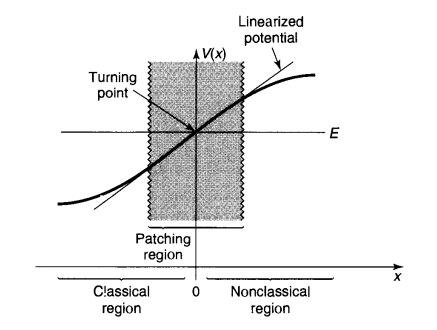
\includegraphics[width=0.6\textwidth]{images/wkb_1}
\end{figure}

This subsection will follow \cite{griffiths2018introduction}. Near a turning point, let us approximate the potential function by linearizing it:
\begin{equation*}
V(x) \approx V(a) + (a-x)V'(a) + \dots
\end{equation*}
To simplify notation we shift the origin and the overall energy so that $a=0$ and $E = V(0) = 0$. Near the turning point, the SE looks like 
\begin{equation*}
-\f{\hbar^2}{2m} \psi''(x) + xV'(0) \psi(x) = 0 \implies \psi''(x) = \f{2m V'(0)}{\hbar^2} x\psi(x).
\end{equation*} 
Define 
\begin{equation*}
\al^3 =  \f{2m V'(0)}{\hbar^2} 
\end{equation*}
and $z = \al x$, so that we get the following ODE:
\begin{equation*}
\boxed{\psi''(z) \psi(z) = z\psi(z)}
\end{equation*}
whose solutions are the \textbf{Airy functions}. This is a second-order equation, so the solution space is spanned by two Airy functions: $Ai(z)$ and $Bi(z)$. \\


\begin{figure}[!htb]
	\centering
	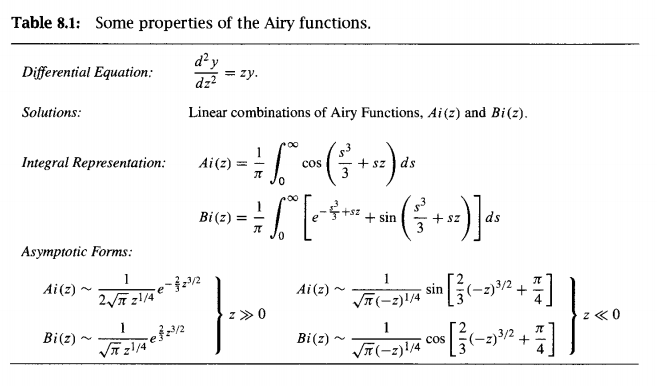
\includegraphics[width=1\textwidth]{images/wkb_2}
	\caption{From \cite{griffiths2018introduction}}
\end{figure}

We see that for $z\ll 0$ the solutions are oscillatory while for $z\gg 0$ we have exponential growth/decay. We can then match up the Airy function near the turning point with the decaying and oscillating
solutions that are valid far from the turning point. This will gives us the \textbf{connection formulae}. \\


Here's the high-level picture: In the classically allowed region we have two oscillating solutions. Near the turning point we have two Airy functions as solutions. In the forbidden region we have two exponentially decaying/growing solutions. At each boundary we have two constraints given by the continuity of $\psi$ and $\psi'$. \\


Now we're ready to looking at the  connection formulae. Consider one turning point. The \textbf{patching wavefunction} $\psi_p(x)$ which connects the inside and outside WKB wavefunctions  is a linear combination of the oscillatory Airy function $Ai(x)$ and the exponential Airy function $Bi(x)$:
\begin{equation*}
\psi_p(x) = a Ai(\al x) + b Bi(\al x).
\end{equation*}

We need to match this to either side of the patching region. These overlap zones are close enough to the turning point that the linearized potential is reasonable accurate, and yet far enough away from the turning point that the WKB approximation is reliable. With this, we see that in the overlap regions, we have 
\begin{equation*}
p(x) \approx \sqrt{2m(E-E-V'(0)x)} = \hbar \al^{3/2}\sqrt{-x}.
\end{equation*}


\begin{figure}[!htb]
	\centering
	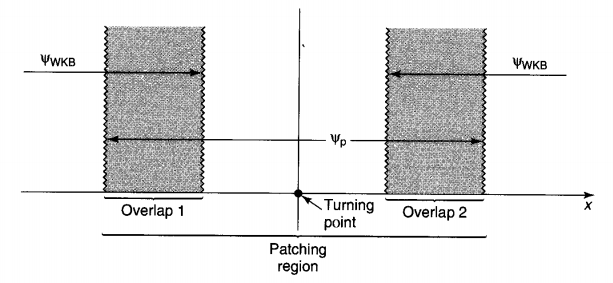
\includegraphics[width=0.75\textwidth]{images/wkb_3}
	\caption{From \cite{griffiths2018introduction}}
\end{figure}



Assuming that the classically forbidden region is $x>0$, we have the WKB wavefunction:
\begin{align*}
\psi(x) = 
\begin{cases}
\f{1}{\sqrt{p(x)}} \lb Be^{(i/\hbar) \int_x^0 p(x')\,dx'} + C e^{(i/\hbar) \int_x^0 p(x')\,dx'}  \rb, &\quad\quad x < 0 \\
\f{1}{\sqrt{\abs{p(x)}} }  De^{-(1/\hbar)\int_0^x \abs{p(x')}\,dx'}, &\quad\quad x > 0
\end{cases}
\end{align*}


Now we match the patching wavefunction to these WKB solutions. In the patching region 2, 
\begin{equation*}
\int_0^x \abs{p(x')}\,dx' \approx \hbar \al^{3/2}\int^x_0 \sqrt{x'}\,dx' = \f{2}{3}\hbar (\al x)^{3/2}.
\end{equation*}
The WKB solution in this region is 
\begin{equation*}
\psi(x) \approx \f{D}{\sqrt{\hbar} \al^{3/4} x^{1/4} } e^{-(2/3)(\al x)^{3/2}},
\end{equation*}
while the patching wavefunction is given by the asymptotic form of the Airy function when $z \gg 0$: 
\begin{equation*}
\psi_p(x) = \f{a}{2\sqrt{\pi} (\al x)^{1/4}} e^{-(2/3) (\al x)^{3/2}} + \f{b}{\sqrt{\pi} (\al x)^{1/4}} e^{+(2/3) (\al x)^{3/2}}.
\end{equation*}
Comparing the two solutions, we must have the following:
\begin{equation*}
\boxed{a = \sqrt{\f{4\pi}{\al \hbar} } D \quad \text{and} \quad b =0}
\end{equation*}


Now we repeat the process for region 1. In the wavefunction-matching process, we must now use the asymptotic form of the Airy function for $z\ll 0$. Finally, comparing the coefficients, one finds that
\begin{equation*}
\boxed{\f{a}{2i\sqrt{\pi} }e^{i\pi /4}  = \f{B}{\sqrt{\hbar \al}} \quad \text{and} \quad \f{-a}{2i \sqrt{\pi}}e^{-i\pi /4} =  \f{C}{\sqrt{\hbar \al}}}
\end{equation*}
From the previous boxed equation, we find 
\begin{equation*}
\boxed{B = -ie^{i\pi/4} D \quad \text{and} \quad C = ie^{-i\pi /4} D} 
\end{equation*}
which puts everything in terms of $D$. These are called the \textbf{connection formulae}, which join the WKB solutions at either side of the turning point. By shifting the turning point back from the origin to some arbitrary $x_2$, the WKB wavefunction becomes
\begin{align*}
\boxed{
\psi(x) \approx 
\begin{cases}
\f{2D}{\sqrt{p(x)}} \sin\lb \f{1}{\hbar} \int_x^{x_2} p(x')\,dx' + \f{\pi}{4} \rb, &\quad\quad x < x_2\\
\f{D}{\sqrt{\abs{p(x)}}} e^{-(1/\hbar) \int_{x_2}^x \abs{p(x')}\,dx'}, &\quad\quad x > x_2.
\end{cases}}
\end{align*}
This situation is with allowed region on the left and forbidden region on the right. We can do the same thing for a setup where the allowed region is on the right and forbidden region on the left. The solution in the latter case is 
\begin{align*}
\boxed{
	\psi(x) \approx 
	\begin{cases}
	\f{D'}{\sqrt{\abs{p(x)}}} e^{-(1/\hbar) \int_{x}^{x_1} \abs{p(x')}\,dx'}, &\quad\quad x < x_1\\
	\f{2D'}{\sqrt{p(x)}} \sin\lb \f{1}{\hbar} \int_{x_1}^{x} p(x')\,dx' + \f{\pi}{4} \rb, &\quad\quad x > x_1
	\end{cases}}
\end{align*}


With these, let's consider some potentials. It turns out the WKB lets us find not just \textbf{quantization rules} but also \textbf{the oscillation of solutions} within the classically allowed region.
\begin{itemize}
	\item \textbf{Potential well with one vertical wall:} Suppose there is a wall at $x=0$. Then we have $\psi(0) = 0$. Assume further that in this situation the left of $x_2$ is allowed but the right is forbidden. 
	
	\begin{figure}[!htb]
		\centering
		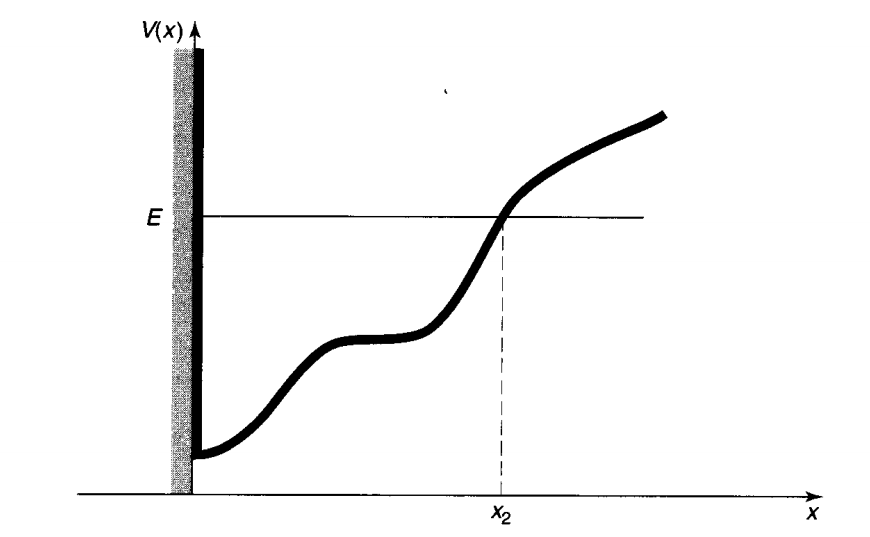
\includegraphics[width=0.75\textwidth]{images/wkb_4}
		\caption{From \cite{griffiths2018introduction}}
	\end{figure}

	To the left of $x_2$, the solution is sinusoidal and must satisfy 
	\begin{align*}
	&\f{1}{\hbar} \int_0^{x_2} p(x')\,dx' + \f{\pi}{4} = n\pi\\
	 &\implies \boxed{\int_0^{x_2} p(x')\,dx' = \lp n - \f{1}{4} \rp\pi \hbar, \quad n = 1,2,3,\dots}
	\end{align*}
	
	
	For this case, consider the example of a \textbf{half-harmonic oscillator}. The potential is 
	\begin{equation*}
	V(x) = \begin{cases}
	\f{1}{2}m\omega^2 x^2, &\quad x > 0\\
	0, &\quad x \leq 0
	\end{cases}
	\end{equation*}
	Then in this case
	\begin{equation*}
	p(x) = \sqrt{2m(E - (1/2) m\omega^2 x^2 )} = m\omega \sqrt{x_2^2 -x^2}
	\end{equation*}
	where the turning point $x_2$ is given by 
	\begin{equation*}
	x_2 = \f{1}{\omega}\sqrt{\f{2E}{m}}.
	\end{equation*}
	This gives
	\begin{equation*}
	\int_0^{x_2}p(x')\,dx' = \dots = \f{\pi E}{2\omega} = \lp n - \f{1}{4} \rp \pi\hbar.
	\end{equation*}
	This leads to
	\begin{equation*}
	E_n = \lp 2n - \f{1}{2}   \rp \hbar \omega, \quad n = 1,2,3,\dots
	\end{equation*}
	
	
	\item \textbf{Potential well with no vertical walls.} In this case, the oscillatory solutions (from patching at the two turning points) must be equal. This means that
	\begin{align*}
	\f{2D'}{\sqrt{p(x)}} \sin\lb \f{1}{\hbar} \int_{x_1}^{x} p(x')\,dx' + \f{\pi}{4} \rb 
	&= \f{2D}{\sqrt{p(x)}} \sin\lb \f{1}{\hbar} \int_x^{x_2} p(x')\,dx' + \f{\pi}{4} \rb \\
	&= -\f{2D}{\sqrt{p(x)}} \sin\lb - \f{1}{\hbar} \int_x^{x_2} p(x')\,dx' - \f{\pi}{4} \rb 
	\end{align*}
	The arguments inside the sine function must be equal (up to $n\pi$). So, we must have
	\begin{equation*}
	\boxed{\int_{x_1}^{x_2} p(x)\,dx = \lp n - \f{1}{2} \rp  \pi \hbar, \quad n = 1,2,\dots}
	\end{equation*}
	This quantization rule allows us to calculate allowed energies, provided the form of the potential $V$.
	
	
	
	\item \textbf{Potential well with two vertical walls.} This is standard stuff:
	\begin{equation*}
	\boxed{\int_{x_1}^{x_2}p(x)\,dx = n\pi \hbar, \quad n = 1,2,\dots}
	\end{equation*}
	
	
	
	\item Problem 8.15 of \cite{griffiths2018introduction} deals with the case of a double well potential. The reader  is highly encouraged to give it a try.
\end{itemize}








\subsection*{Tunneling rates}
WKB can also be used to compute tunneling rates. The tunneling rate is just the transition probability:
\begin{equation*}
T = \f{\abs{F}^2}{\abs{A}^2}  
\end{equation*}


\begin{figure}[!htb]
	\centering
	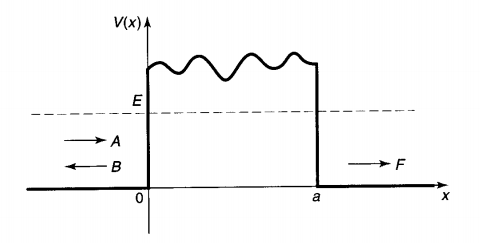
\includegraphics[width=0.7\textwidth]{images/wkb_5}
	\caption{From \cite{griffiths2018introduction}. Potential to be tunneled through.}
\end{figure}



\begin{figure}[!htb]
	\centering
	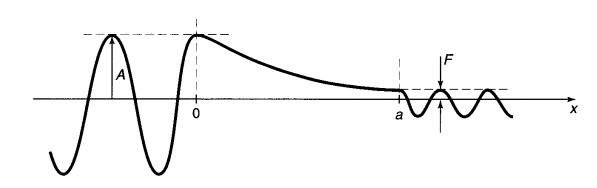
\includegraphics[width=0.7\textwidth]{images/wkb_6}
	\caption{From \cite{griffiths2018introduction}. Tunneling wavefunction.}
\end{figure}


Both the incoming and transmitted wavefunctions are oscillatory. Using WKB, we can calculate $T$. The formula is 
\begin{equation*}
\boxed{T = \f{\abs{F}^2}{\abs{A}^2}   = \exp\lb -\f{2}{\hbar} \int_0^a \abs{p(x)}\,dx \rb \equiv e^{-2\gamma}}
\end{equation*}

From tunneling rates one can also calculate \textbf{lifetimes}. To do this, we use the following conversion rule:
\begin{equation*}
\text{lifetime} = \f{1}{\text{tunnel. prob. per unit time}} \approx \f{1}{T \cdot \text{\# hits per unit time}} = \f{1}{T \f{1}{\tau}} = \f{\tau}{T}
\end{equation*}
where $\tau$ is the period of oscillation between the two turning points in which the particle is trapped. We won't worry too much about lifetime calculations.


%%%%%%%%%%%%%%%%%%%%%%%%%%%%%%%%%%%%%%%
\chapter*{X}
%%%%%%%%%%%%%%%%%%%%%%%%%%%%%%%%%%%%%%%
\chapter*{Y}
%%%%%%%%%%%%%%%%%%%%%%%%%%%%%%%%%%%%%%%
\chapter*{Z}



\section*{Zeeman slower}
%%%%%%%%%%%%%%%%%%%%%%%%%%%%%%%%%%%%%%%






\newpage

\bibliography{Bui_AMO} 
\bibliographystyle{ieeetr}


\end{document}